\documentclass{article}
\usepackage[UTF8, scheme = plain]{ctex} % {ctex} 包用于处理中文支持;[UTF8] 是一种广泛使用的字符编码,支持多种语言的字符,包括中文;[scheme = plain]:设置 ctex 包的样式方案为 plain,plain 方案提供了最基础的中文支持,不包含额外的格式设置或字体调整,适用于那些需要在基本 LaTeX 文档中添加中文支持的场合
\usepackage{fontspec}
\setmainfont{Cochin}
\setCJKmainfont{YuMincho} % macOSにインストールされている場合
\usepackage{amsmath} % 提供额外的环境(如 align, equation, split, multline 等),支持多行公式的对齐和子公式的编号等高级功能
\usepackage{amssymb} % 扩展的数学符号集,通常与 amsmath 宏包一起使用
\usepackage{amsthm} % 用于排版数学定理、定义、证明等结构
\usepackage{graphicx} % 支持在 LaTeX 文档中插入图像(JPEG, PNG, PDF),提供了命令 \includegraphics,可插入、缩放、旋转和裁剪图像
\usepackage{placeins} % 提供了一个命令 \FloatBarrier,可以防止浮动对象(如图片和表格)穿过它。这在保持浮动对象和相应的内容在同一节中非常有用
\usepackage{geometry} % 用于配置页面布局,调整页面尺寸、边距、页脚、页眉等
\usepackage{adjustbox} % 提供了强大的图像调整功能,可以在不改变图片位置的情况下调整其大小
\usepackage{setspace} % 提供了一些简单的方法来设置行间距
\usepackage{indentfirst} % 可以确保每个段落的首行都进行缩进,包括文档中的第一个段落
\usepackage{enumitem} % 用于定制有序列表的序号样式。使用label以自定义序号样式:\begin{enumerate}[label=\arabic*.](\arabic阿拉伯数字,\roman小写罗马数字,\Roman,\alph小写字母,\Alph),“*”之后添加自己喜欢的序号后样式如1.添加“.”,1)添加“)”
\usepackage{wrapfig} % 用于实现文字环绕图片的效果
\usepackage{listings} % 用于插入和格式化代码 \begin{lstlisting} *code* \end{lstlisting}
\usepackage{xcolor}   % 用于颜色设置
\usepackage{lipsum} % For generating dummy text
\usepackage{tocloft} % 用于定制目录样式
\usepackage{floatflt} % For floatflt package
\usepackage{xurl} % 替代 breakurl 宏包,处理长链接
\usepackage[hidelinks]{hyperref} % 使用 hidelinks 选项隐藏链接的方框和颜色
\usepackage{caption} % 为了在非浮动体中使用\captionof
% ps: %%%%%%%%%%%%%%%%%%%%%%%%%%%%%%%%%%%%%%%%%%%%%%%%%%%%%%%%%%%%%%%%%%%%%%%%
% [UTF8, scheme = plain]{ctex}无法输入日语输入法的中点「・」,替代方案:$\cdot$
% 每次修改 [numbers]{natbib} 宏包下的 references.bib 文件后都需要重新编译,以确保所有引用和参考文献都正确更新
% 具体的编译步骤如下:
% >>> xelatex report.tex
% >>> bibtex report
% >>> xelatex report.tex
% >>> xelatex report.tex (是的,这个要输入两遍,以确保所有引用和参考文献都正确显示
%%%%%%%%%%%%%%%%%%%%%%%%%%%%%%%%%%%%%%%%%%%%%%%%%%%%%%%%%%%%%%%%%%%%%%%%%%%%%%

\geometry{left=2cm, right=2cm, top=2.5cm, bottom=2.5cm} % 自定义页边距

% 定义莫兰迪色系的颜色
\definecolor{morandiBackground}{RGB}{245, 245, 245} % 背景
\definecolor{morandiBasic}{RGB}{51, 51, 51}         % 基本文字
\definecolor{morandiKeyword}{RGB}{216, 162, 171}    % 关键字
\definecolor{morandiComment}{RGB}{102, 153, 153}    % 注释
\definecolor{morandiString}{RGB}{151, 190, 130}     % 字符串
\definecolor{morandiNumber}{RGB}{102, 102, 153}     % 行号

% 设置代码的显示风格
\lstset{
  language=Python, % 设置代码语言为 Python
  backgroundcolor=\color{morandiBackground}, % 设置代码区域的背景颜色
  basicstyle=\ttfamily\color{morandiBasic}, % 设置代码字体为等宽字体,颜色
  keywordstyle=\color{morandiKeyword}, % 设置关键字颜色
  commentstyle=\color{morandiComment}, % 设置注释颜色
  stringstyle=\color{morandiString}, % 设置字符串颜色
  numberstyle=\tiny\color{morandiNumber}, % 设置行号的字体和颜色
  breaklines=true, % 启用自动换行
  frame=single, % 为代码区域添加边框
  rulecolor=\color{morandiBasic}, % 设置边框颜色为深灰色
  frameround=tttt, % 设置边框的圆角
  numbers=left, % 在代码左侧显示行号
  numbersep=5pt, % 设置行号和代码之间的间距
  tabsize=2, % 设置制表符的宽度
  showspaces=false, % 不显示空格
  showstringspaces=false % 不显示字符串中的空格
}

% 调整目录的行间距
\setlength{\cftparskip}{0.09cm}  % 你可以根据需要调整这个值

% 调整目录项的缩进(可选)
\cftsetindents{section}{0em}{2em}
\cftsetindents{subsection}{2em}{2.5em}
\cftsetindents{subsubsection}{4.5em}{3em}

\title{\textbf{実験レポート}} % \textbf{文本} 用于将文本变粗
\author{\textbf{洪千宇\ 1223034}}
\date{\today} 

\begin{document}
% \maketitle % 实验报告不需要标题

% 在首页生成目录
\tableofcontents
\newpage % 插入分页符,使正文从新的一页开始

% 1、実験目的%%%%%%%%%%%%%%%%%%%%%%%%%%%%%%%%%%%%%%%%%%%%%%%%
\section{実験目的}
\begin{enumerate}[label=\arabic*), before=\begin{spacing}{1}, after=\end{spacing}] % \arabic阿拉伯数字,\roman小写罗马数字,\Roman,\alph小写字母,\Alph,“*”之后添加自己喜欢的序号后样式, 如1.添加“.”,1)添加“)”;利用{spacing}自定义\item内的行间距
    \item 異なる音源から得られる音声データを用いて、時間ドメインと周波数ドメインでの音の表現の違いを視覚的に比較し、それぞれの有用性を評価する。
    \item 直接音を聞くことと解析ソフトウェアを用いて波形とスペクトルを観察することで、フーリエ解析の原理を体験的に学ぶ。
\end{enumerate}

% 2、実験目的%%%%%%%%%%%%%%%%%%%%%%%%%%%%%%%%%%%%%%%%%%%%%%%%
\section{実験原理}
\begin{spacing}{1.2} % 开始一个有首行缩进的段落,{自定义行间距}
フーリエ解析は、複雑な波形を簡単な波形へ分解する方法であり、その数学的背景にはフーリエ級数、フーリエ変換、そして離散フーリエ変換が含まれている。これらの技術は、周期的な信号を扱う場合にフーリエ級数が、非周期的または無限に広がる信号を扱う場合にフーリエ変換が適用される。
\end{spacing}
\subsection{フーリエ級数展開}
\begin{spacing}{1.2} % 开始一个有首行缩进的段落,{自定义行间距}
    フーリエ級数展開は、周期的な関数を正弦波と余弦波の無限和として表現する方法である。この展開により、任意の周期関数$f(t)$を次のように表すことができる:
    \[f(t) = a_0 + \sum_{n=1}^{\infty} \left( a_n \cos(n \omega_0 t) + b_n \sin(n \omega_0 t) \right)\]
    \indent ここで、$\omega_0 = 2\pi/T$は基本角周波数であり、$a_n$と$b_n$はフーリエ係数である。これらの係数は次の式で計算される:\\
    - $a_0$の計算式:
    \[a_0 = \frac{1}{T} \int_{0}^{T} f(t) \, dt\]
    - $a_n$の計算式:
    \[a_n = \frac{2}{T} \int_{0}^{T} f(t) \cos(n \omega_0 t) \, dt\]
    - $b_n$の計算式:
    \[b_n = \frac{2}{T} \int_{0}^{T} f(t) \sin(n \omega_0 t) \, dt\]
    \indent フーリエ級数展開は、関数が周期的である場合に適用される。一方で、今回の実験で行われた音のフーリエ解析では、非周期的な信号やデジタルデータの分析を行うので、三角フーリエ級数よりも他の手法が一般的に選ばれる。
\end{spacing}

\subsection{(連続)フーリエ変換}
\begin{spacing}{1.2} % 开始一个有首行缩进的段落,{自定义行间距}
    (連続)フーリエ変換は、任意の非周期関数を無限の周期を持つ関数として扱い、その関数を正弦波と余弦波の積分によって表現する手法である。これにより、時間領域の関数を周波数領域に変換することが可能となる。連続フーリエ変換の基本式は以下の通りである:\\
    - フーリエ変換:
    \[F(\omega) = \int_{-\infty}^{\infty} f(t) e^{-i \omega t} \, dt\]
    - 逆フーリエ変換:
    \[f(t) = \frac{1}{2\pi} \int_{-\infty}^{\infty} F(\omega) e^{i \omega t} \, d\omega\]
    \indent ここで、$F(\omega)$は$f(t)$のフーリエ変換であり、複素数形式で周波数領域の表現を提供する。$f(t)$は時間領域の関数であり、$\omega$は角周波数を表す。\\
    \indent 今回の音のフーリエ解析の実験では、連続フーリエ変換は直接使われていない。連続フーリエ変換は理論的には連続的な関数に対して定義され、無限のデータを必要とするため、今回のデジタル信号処理では適用が困難である。
\end{spacing}

\subsection{離散フーリエ変換(DFT)}
\begin{spacing}{1.2} % 开始一个有首行缩进的段落,{自定义行间距}
    離散フーリエ変換(DFT)は、有限個の離散的なデータ点を持つ信号に対して周波数成分を分析する手法である。この変換は、デジタル信号を複素数の周波数スペクトルに変換し、各成分の振幅と位相情報を提供できる。離散フーリエ変換の計算式は以下となる:
    \[X[k] = \sum_{n=0}^{N-1} x[n] e^{-i 2\pi kn/N}\]
    \indent フーリエ変換と離散フーリエ変換(DFT)は似たような概念であり、信号の周波数成分を分析するために使用されるが、今回の音のフーリエ解析の実験で離散フーリエ変換が連続フーリエ変換よりも適用されたのは、実験で取得されるデータがデジタル形式であり、有限かつ離散的なサンプルから構成されるためである。連続フーリエ変換は理論的には無限の連続データを扱うため、デジタル信号には適用が困難である。一方で、DFTは有限のデータポイントに基づいて計算を行うため、デジタル信号処理に最適であり、効率的に周波数成分を分析できる。これにより、サンプル化された音声データの周波数特性を正確に捉え、解析することが可能となる。
\end{spacing}

\subsection{高速フーリエ変換(FFT)}
\begin{spacing}{1.2} % 开始一个有首行缩进的段落,{自定义行间距}
    高速フーリエ変換(FFT)は、離散フーリエ変換(DFT)を計算するための効率的なアルゴリズムである。FFTは、計算の複雑さを大幅に削減し、特にデータ点数が多い場合にその効果が顕著である。\\
    \indent FFTの基本的な考え方は、「分割統治法」[2]に基づいている。FFTでは、信号$x[n]$を$x[2m]$(偶数インデックス)と$x[2m+1]$(奇数インデックス)に分け、それぞれに対してDFTを行う。この過程は再帰的に行われ、計算量を減少させる。
    \[X[k] = \sum_{m=0}^{N/2-1} x[2m] e^{-i 2\pi k(2m)/N} + \sum_{m=0}^{N/2-1} x[2m+1] e^{-i 2\pi k(2m+1)/N}\]
    \indent ここで、第一項は$N/2$点DFTの偶数成分、第二項は奇数成分を表す。各項はさらに分割して計算が可能であり、この分割により通常のDFTの計算量$O(N^2)$が$O(N\log N)$に削減される。
\end{spacing}
\begin{figure}[ht] % 选项 [htbp] 代表位置优先级, “here, top, bottom, page” 分别表示:此处、页顶、页底、单独一页
    \centering
    \adjincludegraphics[width=0.8\textwidth, keepaspectratio]{/Users/kiloverse/Documents/物理学実験2/音のフーリエ解析/data/report_figs/fft.png}
    \caption{FFT分割統治法[2]}
\end{figure}
\FloatBarrier
\begin{spacing}{1.2} % 开始一个有首行缩进的段落,{自定义行间距}
    高速フーリエ変換(FFT)は特にサンプル数が2のべき乗である場合に最も効率的であるため、デジタル信号処理、画像処理、音響分析など多くの科学技術分野で広く利用されている。今回の音のフーリエ解析の実験では、SignalScope Basic 2022というソフトウェアにFFT計算機能が内蔵されており、時間分布から直接に周波数分布の結果を得ることができる。ただし、自分で計算を行う場合には、Pythonなどのプログラミング言語に用意されているFFTの計算モジュールを使用することで、さまざまな方法で計算を実行することができる。
\end{spacing}

\section{実験方法}

\subsection{実験装置}
\begin{spacing}{1.2}
    実験には、(SignalScope Basic 2022ソフトウェアがインストールされた)コンピュータ、オーディオミキサー、USB Audio Adapter、マイク、モニター用スピーカーが用いられる。これらの装置は、音声信号の取得、調整、分析を行うためにセットアップされる。
\end{spacing}{1.2}

\subsection{実験手順}
\subsubsection{実験1:母音の特徴}
\begin{enumerate}[label=\arabic*)]
    \item マイクを通じて母音「あ」「い」「う」「え」「お」の音声を発音した。
    \item 各母音の音声データを「Oscilloscope」と「FFT Analyzer」モードで時間ドメインの波形と周波数スペクトル観察し、データ取得を取得した。
    \item 「Spectrogram」モードで5つの母音の周波数時間分布を比較しながら観察できた。
\end{enumerate}

\subsubsection{実験2:和音の分析}
\begin{enumerate}[label=\arabic*)]
    \item 「ド」の録音を入力して、その特徴を捉えた。
    \item 和音の録音を入力として、それぞれの和音の特徴的な波形図と周波数成分を観察した。
    \item 音階テーブルを参考し、各和音の3つの構成音を調べた。
\end{enumerate}
\begin{figure}[ht] % 选项 [htbp] 代表位置优先级, “here, top, bottom, page” 分别表示:此处、页顶、页底、单独一页
    \centering
    \fbox{\adjincludegraphics[width=0.7\textwidth, keepaspectratio]{/Users/kiloverse/Documents/物理学実験2/音のフーリエ解析/data/report_figs/実験1配置図.png}}
    \caption{実験1配置図}
\end{figure}
\FloatBarrier

\subsubsection{実験3:特徴的な波形の分析}
\begin{enumerate}[label=\arabic*)]
    \item Fourier: Making Waves サイト[3]から余弦波、三角波、矩形波、及びノコギリ波を作った。
    \item それぞれの波形を入力として、OscilloscopeとFFTのデータを取得した。
    \item 波形の形状が音色にどのように影響するかを音を耳で聞いて、フーリエ級数を体得した。
\end{enumerate}

\subsubsection{実験4.1:ギターの普通奏法とハーモニックス奏法}
\begin{enumerate}[label=\arabic*)]
    \item ギターの普通奏法として、弦の中央部を押しながら弾いた音と押さずに弾いた音を入力として、波形図を周波数分布のデータを取得した。
    \item ギターのハーモニックス奏法として、弦の2分点・3分点・4分点のところを軽く触れながら弾いた音を入力として、波形図を周波数分布のデータを取得した。
    \item 普通奏法とハーモニックス奏法の周波数成分の差異を評価した。
\end{enumerate}

\subsubsection{実験4.2:様々な楽器の振動}
\begin{enumerate}[label=\arabic*)]
    \item パンパイプ、トランペット、人の口笛など、他の楽器の振動を入力として、波形図を周波数分布のデータを取得した。
    \item 各楽器がどのようにしてその特有の音色を生み出しているかを、周波数成分の特徴から調べた。
\end{enumerate}
\begin{figure}[ht] % 选项 [htbp] 代表位置优先级, “here, top, bottom, page” 分别表示:此处、页顶、页底、单独一页
    \centering
    \fbox{\adjincludegraphics[width=0.7\textwidth, keepaspectratio]{/Users/kiloverse/Documents/物理学実験2/音のフーリエ解析/data/report_figs/実験4配置図.png}}
    \caption{実験4配置図}
\end{figure}
\FloatBarrier

% 4、実験結果%%%%%%%%%%%%%%%%%%%%%%%%%%%%%%%%%%%%%%%%%%%%%%%%

\section{実験結果$\cdot$実験考察}
今回の実験では多くのデータが得られたため、便宜上に実験別に結果と考察を記述することとした。

\subsection{実験1:母音の特徴}
\subsubsection{実験1結果}
\begin{spacing}{1.2}
    「あ」「い」「う」「え」「お」の周波数分布と波形図の結果は以下となる。特に、特徴を易く捉えるように、0.00s から 0.03s の間の波形を抽出した。
\end{spacing}
\begin{figure}[ht] % 选项 [htbp] 代表位置优先级, “here, top, bottom, page” 分别表示:此处、页顶、页底、单独一页
    \centering
    \fbox{\adjincludegraphics[width=0.98\textwidth, keepaspectratio]{/Users/kiloverse/Documents/物理学実験2/音のフーリエ解析/data/report_figs/あ結果.png}}
    \caption{「あ」の結果}
\end{figure}
\begin{figure}[ht] % 选项 [htbp] 代表位置优先级, “here, top, bottom, page” 分别表示:此处、页顶、页底、单独一页
    \centering
    \fbox{\adjincludegraphics[width=0.98\textwidth, keepaspectratio]{/Users/kiloverse/Documents/物理学実験2/音のフーリエ解析/data/report_figs/い結果.png}}
    \caption{「い」の結果}
\end{figure}
\begin{figure}[ht] % 选项 [htbp] 代表位置优先级, “here, top, bottom, page” 分别表示:此处、页顶、页底、单独一页
    \centering
    \fbox{\adjincludegraphics[width=0.98\textwidth, keepaspectratio]{/Users/kiloverse/Documents/物理学実験2/音のフーリエ解析/data/report_figs/う結果.png}}
    \caption{「う」の結果}
\end{figure}
\begin{figure}[ht] % 选项 [htbp] 代表位置优先级, “here, top, bottom, page” 分别表示:此处、页顶、页底、单独一页
    \centering
    \fbox{\adjincludegraphics[width=0.98\textwidth, keepaspectratio]{/Users/kiloverse/Documents/物理学実験2/音のフーリエ解析/data/report_figs/え結果.png}}
    \caption{「え」の結果}
\end{figure}
\begin{figure}[ht] % 选项 [htbp] 代表位置优先级, “here, top, bottom, page” 分别表示:此处、页顶、页底、单独一页
    \centering
    \fbox{\adjincludegraphics[width=0.98\textwidth, keepaspectratio]{/Users/kiloverse/Documents/物理学実験2/音のフーリエ解析/data/report_figs/お結果.png}}
    \caption{「お」の結果}
\end{figure}
\FloatBarrier

また、「あ」「い」「う」「え」「お」を比較しながら見えるように、周波数時間分布を描いたSpectrogramの結果は以下となる。
\begin{figure}[ht] % 选项 [htbp] 代表位置优先级, “here, top, bottom, page” 分别表示:此处、页顶、页底、单独一页
    \centering
    \fbox{\adjincludegraphics[width=0.7\textwidth, keepaspectratio]{/Users/kiloverse/Documents/物理学実験2/音のフーリエ解析/data/report_figs/あいうえおspectrogram.png}}
    \caption{母音のspectrogram}
\end{figure}
\FloatBarrier

\subsubsection*{課題1-1:結果の解析}
\begin{spacing}{1.2}
以上の結果から、各母音のスペクトルには明確な相違点と共通点が観察された。\\
- 共通点:
\begin{itemize}
    \item \textbf{基本周波数の存在}:すべての母音において、基本周波数が存在し、それが明瞭に観測された。これは母音の発声において、声帯の振動が基礎となる周波数を生成していることを示している。
    \item \textbf{ハーモニクスの存在}:各母音のスペクトルには、基本周波数の整数倍となる倍音が存在し、これらが母音の音色を形成する要素として機能していた。
    \item \textbf{低周波数のエネルギーが強い}:すべての母音において、低周波数帯域のエネルギーが強く、これは母音が発音される際に低周波数成分が豊富に生成されることを反映している。
\end{itemize}
- 相違点:
\begin{itemize}
    \item \textbf{スペクトルの強度}:母音によってスペクトルの強度分布にも差がある。例えば、「お」のスペクトルが比較的強いハーモニクスを示していたのに対し、「い」は強い低周波数を示していた。それらの違いは、母音の発音位置や口腔内の形状が変化することによるものであり、特定のフォルマント頻度が強調されることが原因だと推測する。
    \item \textbf{スペクトログラムの特徴}:スペクトログラムは音声信号の時間経過に対する周波数の分布を示しており、理論的にはフォルマントの位置変化を視覚的に捉えることができる。しかし、低周波数のエネルギーが自然に強いため、全体のダイナミックレンジを平均化する処理を施さない限り、定量的なフォルマントの識別は困難である。ただし、高い周波数領域の相違は明瞭であり、これにより母音の識別が可能である。
\end{itemize}
\end{spacing}

\subsubsection{考察1:母音の識別する方法}
\begin{spacing}{1.2}
    今回の実験ではプリエンファシスフィルタが適用された録音データがないため、フォルマントから母音を識別することが困難である。また、周波数分布は時間の経過とともに、さらに話者(子供、女性、男性)によっても変化するため、直接周波数分布から母音を識別することは困難である。このため、フォルマント以外の別の2つの方法についても考察を進める。
\end{spacing}
\subsubsection*{(1) 累積スペクトル}
\begin{spacing}{1.2}
    時間を通じて継続的に発声される音声データを処理したい場合、累積スペクトル法が適用される。
    
    累積スペクトルは、特定時間内の周波数成分の強度を積算し、その累積値を用いて音声の特徴を抽出する。この分析により、時間経過に伴う周波数の変化を捉え、母音の特徴を明確にする。
    
    例えば、図11に示される累積スペクトルは、母音「い」と「う」の高い周波数のところでは差異が現れている[4]。母音/う/の$2.6KHz$付近で累積スペクトルが谷になっていて,これは音声/ウ/の全てにおいて見られる共通した特徴となっている。
    
    このように、各母音の特有のフィーチャーを用いることで、より精確な母音識別が可能であると考えられる。
\end{spacing}
\begin{figure}[htbp]
    \centering
    \begin{minipage}[b]{0.5\textwidth} % minipage 环境用于在同一行内并排放置内容,[b] 参数表示底部对齐,{0.5\textwidth} 设置 minipage 的宽度为页面宽度的一半
      \centering
      \adjustbox{height=0.4\textheight,keepaspectratio}{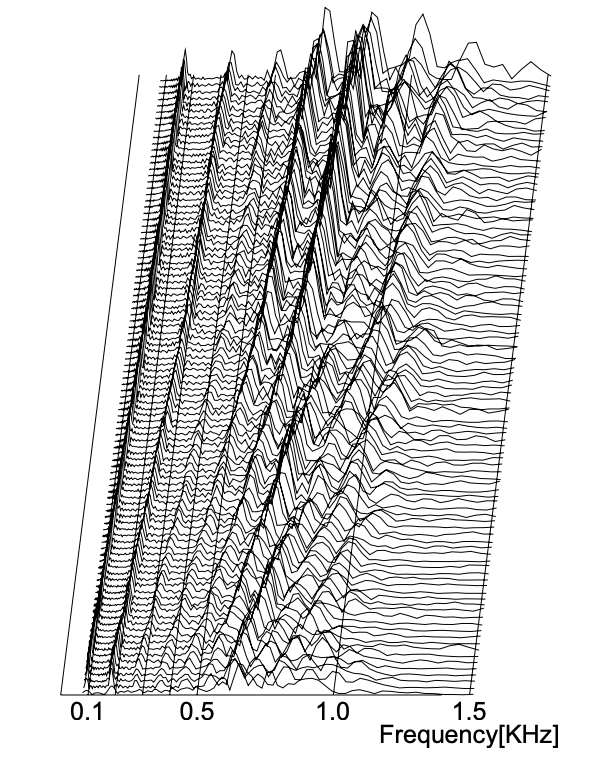
\includegraphics{/Users/kiloverse/Documents/物理学実験2/音のフーリエ解析/data/report_figs/累積スペクトル_aの時間発展.png}}
      \caption{継続的な音声データの例[4]}
    \end{minipage}% % 在两个 minipage 环境之间使用 % 符号来消除之间的空白
    \begin{minipage}[b]{0.5\textwidth}
      \centering
      \adjustbox{height=0.4\textheight,keepaspectratio}{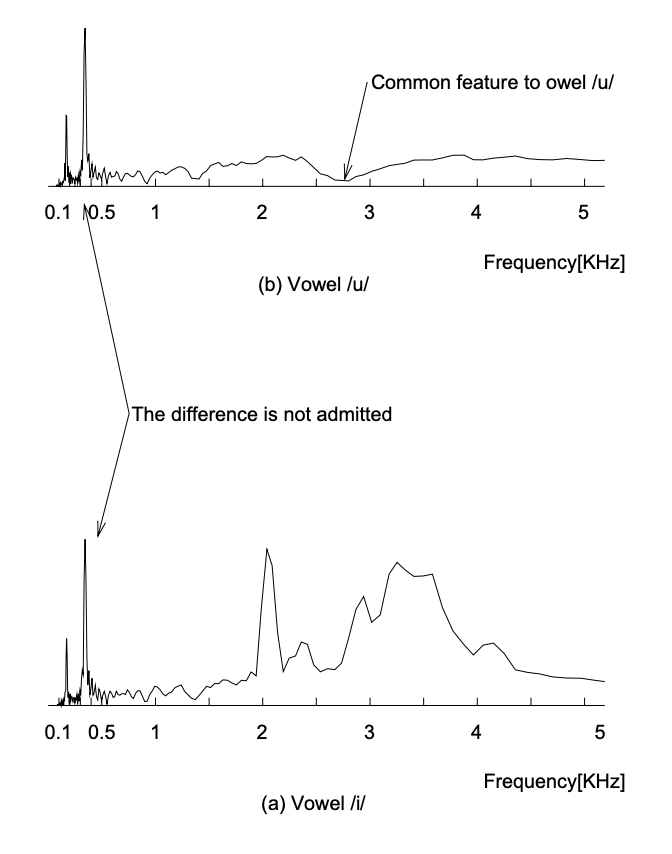
\includegraphics{/Users/kiloverse/Documents/物理学実験2/音のフーリエ解析/data/report_figs/累積スペクトル_iとuの比較.png}}
      \caption{/う/と/い/の累積スペクトルの例[4]} 
    \end{minipage}
\end{figure}
\FloatBarrier

\subsubsection*{(2) 周波数振幅比率}
\begin{spacing}{1.2}
    周波数振幅比率は、全周波数成分の振幅の合計に対する各成分の振幅の比率を計算し、母音の特徴を定量的に評価する手法である。この方法は、短時間での発声データに適用され、特に母音の短い発声から周波数成分の相対的な強度を評価するのに適している。

    5つの母音の認識基準は下の表1から表5の通りである[5]。
    \begin{figure}[ht] % 选项 [htbp] 代表位置优先级, “here, top, bottom, page” 分别表示:此处、页顶、页底、单独一页
        \centering
        \adjincludegraphics[width=0.99\textwidth, keepaspectratio]{/Users/kiloverse/Documents/物理学実験2/音のフーリエ解析/data/report_figs/母音の識別基準.png}
        \caption{母音の識別基準[5]}
    \end{figure}
    \FloatBarrier
    この表の使い方として、例えば母音領域の任意の区間をフーリエ解析して、
    周波数成分毎の振幅比率を求めたときに、
    青い区間に該当する全ての周波数成分の振幅比率が3\%以下で、周波数700Hzから1000Hzの薄い赤色の区間に振幅比率3.8\%以上の周波数成分が3個以上存在し、
    更に1200Hzから1700Hzの薄い赤色区間に振幅比率3.8\%以上の周波数成分が1個以上存在するという条件が満たされた時に、この分析区間は「あ」であると判定する。
    
    この音声認識法によって、振幅比率に大きく影響を与えない程度の強さのノイズは無視できることになる。音声認識結果を何パーセントの確からしさといった確率で表現するのではなく、特定の周波数スペクトルパターンが「ある」か「ない」かの2値で、単純に求めることにその特徴がある。
\end{spacing}

\newpage

\subsection{実験2:和音の分析}
\subsubsection{実験2結果}
    \begin{spacing}{1.2}
    まず、「ド.mp3」を入力として、観測できた波形図と周波数スペクトルの結果は以下となる。
    \begin{figure}[ht] % 选项 [htbp] 代表位置优先级, “here, top, bottom, page” 分别表示:此处、页顶、页底、单独一页
        \centering
        \fbox{\adjincludegraphics[width=0.97\textwidth, keepaspectratio]{/Users/kiloverse/Documents/物理学実験2/音のフーリエ解析/data/report_figs/実験2ド.png}}
        \caption{「ド」の結果}
    \end{figure}
    \FloatBarrier
    次に、「和音1.mp3」〜「和音6.mp3」を入力として、観測できた波形図と周波数スペクトルの結果は以下となる。
    \begin{figure}[ht] % 选项 [htbp] 代表位置优先级, “here, top, bottom, page” 分别表示:此处、页顶、页底、单独一页
        \centering
        \fbox{\adjincludegraphics[width=0.97\textwidth, keepaspectratio]{/Users/kiloverse/Documents/物理学実験2/音のフーリエ解析/data/report_figs/実験2_osc_12.png}}
        \caption{「和音1」と「和音2」の波形図}
    \end{figure}
    \begin{figure}[ht] % 选项 [htbp] 代表位置优先级, “here, top, bottom, page” 分别表示:此处、页顶、页底、单独一页
        \centering
        \fbox{\adjincludegraphics[width=0.97\textwidth, keepaspectratio]{/Users/kiloverse/Documents/物理学実験2/音のフーリエ解析/data/report_figs/実験2_osc_34.png}}
        \caption{「和音3」と「和音4」の波形図}
    \end{figure}
    \begin{figure}[ht] % 选项 [htbp] 代表位置优先级, “here, top, bottom, page” 分别表示:此处、页顶、页底、单独一页
        \centering
        \fbox{\adjincludegraphics[width=0.97\textwidth, keepaspectratio]{/Users/kiloverse/Documents/物理学実験2/音のフーリエ解析/data/report_figs/実験2_osc_56.png}}
        \caption{「和音5」と「和音6」の波形図}
    \end{figure}
    \begin{figure}[ht] % 选项 [htbp] 代表位置优先级, “here, top, bottom, page” 分别表示:此处、页顶、页底、单独一页
        \centering
        \fbox{\adjincludegraphics[width=0.97\textwidth, keepaspectratio]{/Users/kiloverse/Documents/物理学実験2/音のフーリエ解析/data/result_plot/2_fft_id_wa1.png}}
        \caption{「和音1」の周波数スペクトル}
    \end{figure}
    \begin{figure}[ht] % 选项 [htbp] 代表位置优先级, “here, top, bottom, page” 分别表示:此处、页顶、页底、单独一页
        \centering
        \fbox{\adjincludegraphics[width=0.97\textwidth, keepaspectratio]{/Users/kiloverse/Documents/物理学実験2/音のフーリエ解析/data/result_plot/2_fft_id_wa2.png}}
        \caption{「和音2」の周波数スペクトル}
    \end{figure}
    \begin{figure}[ht] % 选项 [htbp] 代表位置优先级, “here, top, bottom, page” 分别表示:此处、页顶、页底、单独一页
        \centering
        \fbox{\adjincludegraphics[width=0.97\textwidth, keepaspectratio]{/Users/kiloverse/Documents/物理学実験2/音のフーリエ解析/data/result_plot/2_fft_id_wa3.png}}
        \caption{「和音3」の周波数スペクトル}
    \end{figure}
    \begin{figure}[ht] % 选项 [htbp] 代表位置优先级, “here, top, bottom, page” 分别表示:此处、页顶、页底、单独一页
        \centering
        \fbox{\adjincludegraphics[width=0.97\textwidth, keepaspectratio]{/Users/kiloverse/Documents/物理学実験2/音のフーリエ解析/data/result_plot/2_fft_id_wa4.png}}
        \caption{「和音4」の周波数スペクトル}
    \end{figure}
    \begin{figure}[ht] % 选项 [htbp] 代表位置优先级, “here, top, bottom, page” 分别表示:此处、页顶、页底、单独一页
        \centering
        \fbox{\adjincludegraphics[width=0.97\textwidth, keepaspectratio]{/Users/kiloverse/Documents/物理学実験2/音のフーリエ解析/data/result_plot/2_fft_id_wa5.png}}
        \caption{「和音5」の周波数スペクトル}
    \end{figure}
    \begin{figure}[ht] % 选项 [htbp] 代表位置优先级, “here, top, bottom, page” 分别表示:此处、页顶、页底、单独一页
        \centering
        \fbox{\adjincludegraphics[width=0.97\textwidth, keepaspectratio]{/Users/kiloverse/Documents/物理学実験2/音のフーリエ解析/data/result_plot/2_fft_id_wa6.png}}
        \caption{「和音6」の周波数スペクトル}
    \end{figure}
    \FloatBarrier
    \subsubsection*{結果の解析}
    まず、図15より、「ド」音(C5)の基本振動数は524Hzであり、基本振動数の倍数である1048Hz、1576Hz、2108Hz、2644Hz、3192Hzといったハーモニクスも観察された。基本振動数のピークが最も大きく、ハーモニクスのピークは基本振動数から遠ざかるにつれて徐々に小さくなっていることが分かった。
    また、オシロスコープで観察された「ド」音の時間波形データは、正弦波形に近くて、これは音の振動が非常に安定していることを表している。

    次に、図17から図22に示された和音1〜和音6の周波数分布は、複数の明確な基本振動数を示し、それに関連するハーモニクスも観察された。
    これらの周波数成分は、和音を形成する各音階の特性を反映している。(具体的音階の識別は後の考察でさらに詳細に説明する。)
    また、波形図においては、和音の複雑さが振幅の不安定さとして表れる。
    波形が不規則に見えるのは、異なる周波数の波が重なり合って干渉する結果だと考察する。
    この干渉により、波形は一定のリズムを持たず、振幅も不安定になった。
    
    ピアノ音の音色を形成する重要な要素として、ハーモニクスが観察された。
    ピアノの弦がハンマーに打たれると、弦全体が振動し始め、この振動が音として発生し、基本振動に加えて、弦の長さの分数的な位置でのノードを持つ様々なモードで発生する。これがハーモニクスを生成し、ピアノ特有の豊かな音色を作り出した。
    \end{spacing}
\vspace{110pt} % 每行大约12pt
\subsubsection{課題2-1:和音の構成音の分析}
    \begin{spacing}{1.2}
        和音1~和音6は3つの音から構成されているので、これからその3音の基本振動数を割り出してみる。平均律の音階の振動数は下表の通りである。
        \begin{table}[ht] % 选项 [htbp] 代表位置优先级, “here, top, bottom, page” 分别表示:此处、页顶、页底、单独一页
            \centering
            \fbox{\adjincludegraphics[width=0.98\textwidth, keepaspectratio]{/Users/kiloverse/Documents/物理学実験2/音のフーリエ解析/data/report_figs/音階の振動数.png}}
            \caption{音階の振動数}
        \end{table}
        \subsubsection*{和音1}
        下図の和音1の周波数成分について、各ピークがより明瞭に見えるように、y軸をログスケールに設定した。また、基本振動数に基づき、ピークを3つのグループに分け、それぞれ異なる色で表示した。さらに、平均律の音階の振動数を参照し、和音の基本振動数及びそれに対応する音階を自動的に識別し、出力できるプログラムを作成した。
        結果は下記の通りであり、和音1の構成音が\underline{C5、E5、G5}とわかった。
        \begin{figure}[ht] % 选项 [htbp] 代表位置优先级, “here, top, bottom, page” 分别表示:此处、页顶、页底、单独一页
            \centering
            \fbox{\adjincludegraphics[width=0.7\textwidth]{/Users/kiloverse/Documents/物理学実験2/音のフーリエ解析/data/result_plot/2_fft_log_id13-6_wa1.png}}
            \caption{和音1の周波数成分(y in logscale)}
        \end{figure}
        \FloatBarrier
        \begin{lstlisting}
# 和音1の構成音:
Fundamental frequency 524.00 Hz is closest to C5
Fundamental frequency 660.00 Hz is closest to E5
Fundamental frequency 785.00 Hz is closest to G5
        \end{lstlisting}

        \subsubsection*{和音2}
        以下の和音2の周波数成分と構成音の結果によって、和音2の構成音が\underline{F5、A5、C6}とわかった。
        \begin{figure}[ht] % 选项 [htbp] 代表位置优先级, “here, top, bottom, page” 分别表示:此处、页顶、页底、单独一页
            \centering
            \fbox{\adjincludegraphics[width=0.7\textwidth]{/Users/kiloverse/Documents/物理学実験2/音のフーリエ解析/data/result_plot/2_fft_log_id13-6_wa2.png}}
            \caption{和音2の周波数成分(y in logscale)}
        \end{figure}
        \FloatBarrier
        \begin{lstlisting}
# 和音2の構成音:
Fundamental frequency 700.00 Hz is closest to F5
Fundamental frequency 884.00 Hz is closest to A5
Fundamental frequency 1048.00 Hz is closest to C6
        \end{lstlisting}
        \subsubsection*{和音3}
        以下の和音3の周波数成分と構成音の結果によって、和音3の構成音が\underline{G5、B5、D6}とわかった。
        \begin{figure}[ht] % 选项 [htbp] 代表位置优先级, “here, top, bottom, page” 分别表示:此处、页顶、页底、单独一页
            \centering
            \fbox{\adjincludegraphics[width=0.7\textwidth]{/Users/kiloverse/Documents/物理学実験2/音のフーリエ解析/data/result_plot/2_fft_log_id13-6_wa3.png}}
            \caption{和音3の周波数成分(y in logscale)}
        \end{figure}
        \FloatBarrier
        \begin{lstlisting}
# 和音3の構成音:
Fundamental frequency 788.00 Hz is closest to G5
Fundamental frequency 992.00 Hz is closest to B5
Fundamental frequency 1176.00 Hz is closest to D6
        \end{lstlisting}
        \subsubsection*{和音4}
        以下の和音4の周波数成分と構成音の結果によって、和音4の構成音が\underline{E5、G5、C6}とわかった。
        \begin{figure}[ht] % 选项 [htbp] 代表位置优先级, “here, top, bottom, page” 分别表示:此处、页顶、页底、单独一页
            \centering
            \fbox{\adjincludegraphics[width=0.7\textwidth]{/Users/kiloverse/Documents/物理学実験2/音のフーリエ解析/data/result_plot/2_fft_log_id13-6_wa4.png}}
            \caption{和音4の周波数成分(y in logscale)}
        \end{figure}
        \FloatBarrier
        \begin{lstlisting}
# 和音4の構成音:
Fundamental frequency 660.00 Hz is closest to E5
Fundamental frequency 788.00 Hz is closest to G5
Fundamental frequency 1048.00 Hz is closest to C6
        \end{lstlisting}
        \subsubsection*{和音5}
        以下の和音5の周波数成分と構成音の結果によって、和音5の構成音が\underline{C5、D\#5、G5}とわかった。
        \begin{figure}[ht] % 选项 [htbp] 代表位置优先级, “here, top, bottom, page” 分别表示:此处、页顶、页底、单独一页
            \centering
            \fbox{\adjincludegraphics[width=0.7\textwidth]{/Users/kiloverse/Documents/物理学実験2/音のフーリエ解析/data/result_plot/2_fft_log_id13-6_wa5.png}}
            \caption{和音5の周波数成分(y in logscale)}
        \end{figure}
        \FloatBarrier
        \begin{lstlisting}
# 和音5の構成音:
Fundamental frequency 524.00 Hz is closest to C5
Fundamental frequency 624.00 Hz is closest to D#5
Fundamental frequency 788.00 Hz is closest to G5
        \end{lstlisting}
        \subsubsection*{和音6}
        以下の和音6の周波数成分と構成音の結果によって、和音6の構成音が\underline{C5、E5、A5}とわかった。
        \begin{figure}[ht] % 选项 [htbp] 代表位置优先级, “here, top, bottom, page” 分别表示:此处、页顶、页底、单独一页
            \centering
            \fbox{\adjincludegraphics[width=0.7\textwidth]{/Users/kiloverse/Documents/物理学実験2/音のフーリエ解析/data/result_plot/2_fft_log_id13-6_wa6.png}}
            \caption{和音6の周波数成分(y in logscale)}
        \end{figure}
        \FloatBarrier
        \begin{lstlisting}
# 和音6の構成音:
Fundamental frequency 524.00 Hz is closest to C5
Fundamental frequency 660.00 Hz is closest to E5
Fundamental frequency 884.00 Hz is closest to A5
        \end{lstlisting}
    \end{spacing}
\newpage
\subsubsection{考察2:平均律と純正律[6]}
    \begin{spacing}{1.2}
        今回のピアノの音階の実験では、ピアノが「平均律」に調律されていることが前提となっている。それに対して、純正律というものも存在しており、以下では平均律と純正律を比較しながら説明していく。
        \subsubsection*{平均律(Equal Temperament)}
        平均律は、オクターヴを12の等しい半音に分割するチューニングシステムで、隣接する音の周波数比は常に \(2^{1/12}\) と一定である。平均律の主な特徴と利点は以下の通りである:
        \begin{enumerate}[label=\arabic*), before=\begin{spacing}{1.2}, after=\end{spacing}] % \arabic阿拉伯数字,\roman小写罗马数字,\Roman,\alph小写字母,\Alph,“*”之后添加自己喜欢的序号后样式, 如1.添加“.”,1)添加“)”;利用{spacing}自定义\item内的行间距
            \item \textbf{転調の自由度}:平均律ではどのキーから始めても同じ音間隔が保たれるため、転調しても演奏や和音の感じが変わらない。これにより、作曲や演奏が容易になり、現代音楽の多様性を支えている。
            \item \textbf{均一な音色}:全ての鍵盤やフレットが均等にチューニングされているため、どの音を弾いても一貫した音色と調和を得ることができる。
        \end{enumerate}
        \begin{figure}[ht] % 选项 [htbp] 代表位置优先级, “here, top, bottom, page” 分别表示:此处、页顶、页底、单独一页
            \centering
            \adjincludegraphics[height=0.15\textwidth]{/Users/kiloverse/Documents/物理学実験2/音のフーリエ解析/data/report_figs/平均律.png}
            \caption{平均律の音階[6]}
        \end{figure}
        \FloatBarrier
        \subsubsection*{純正律(Just Intonation)}
        純正律は、自然な音響的な整数比に基づいて音をチューニングするシステムで、その主な特徴は以下の通りである:
        \begin{enumerate}[label=\arabic*), before=\begin{spacing}{1.2}, after=\end{spacing}] % \arabic阿拉伯数字,\roman小写罗马数字,\Roman,\alph小写字母,\Alph,“*”之后添加自己喜欢的序号后样式, 如1.添加“.”,1)添加“)”;利用{spacing}自定义\item内的行间距
            \item \textbf{調和の美}:純正律では、完全な整数比(例:2:1、3:2、5:4)に基づいて音をチューニングするため、特定の調では和音が非常に純粋で調和が取れた響きを生み出せる。純正律でチューニングされた和音は、非常に調和が取れており、リスナーにとって心地よい響きを提供する。
            \item \textbf{音楽表現の豊かさ}:純正律は、演奏される音楽の感情的な深みを増すことができ、表現の幅を広げることが可能である。
            \item \textbf{限定された転調}:純正律では特定の調に最適化されているため、他の調に転調すると音が不協和に聞こえることがある。
        \end{enumerate}
        \begin{figure}[ht] % 选项 [htbp] 代表位置优先级, “here, top, bottom, page” 分别表示:此处、页顶、页底、单独一页
            \centering
            \adjincludegraphics[height=0.15\textwidth]{/Users/kiloverse/Documents/物理学実験2/音のフーリエ解析/data/report_figs/純正律.png}
            \caption{純正律の音階[6]}
        \end{figure}
        \FloatBarrier
        \newpage
        自分の耳で平均律と純正律の曲の違いを体験するために、両調律の曲の例を調査した。
        
        平均律の例として、以下の曲が挙げられている:
        \begin{enumerate}[label=\arabic*), before=\begin{spacing}{1.2}, after=\end{spacing}] % \arabic阿拉伯数字,\roman小写罗马数字,\Roman,\alph小写字母,\Alph,“*”之后添加自己喜欢的序号后样式, 如1.添加“.”,1)添加“)”;利用{spacing}自定义\item内的行间距
            \item Johann Sebastian Bach - Prelude 1 in C Major\\
            \url{https://www.youtube.com/watch?v=gVah1cr3pU0}
            \item Ludwig van Beethoven - Piano Sonata No. 14 "Moonlight" in C sharp minor\\
            \url{https://www.youtube.com/watch?v=rlJHNufol8Q}
        \end{enumerate}

        純正律の例として、以下の曲が挙げられている:
        \begin{enumerate}[label=\arabic*), before=\begin{spacing}{1.2}, after=\end{spacing}] % \arabic阿拉伯数字,\roman小写罗马数字,\Roman,\alph小写字母,\Alph,“*”之后添加自己喜欢的序号后样式, 如1.添加“.”,1)添加“)”;利用{spacing}自定义\item内的行间距
            \item Thomas Tallis - Spem in alium\\
            \url{https://www.youtube.com/watch?v=7iHunHKvKd4}
            \item Giovanni Pierluigi da Palestrina - Missa Papae Marcelli\\
            \url{https://www.youtube.com/watch?v=BRfF7W4El60}
        \end{enumerate}

        理論的には、純正律での演奏は和音の純度が非常に高く、特定のキーでの演奏が非常に美しい一方、平均律では任意のキーへの移行がスムーズで、現代の多様な音楽スタイルに適応している。実際にこれらの曲を聴いたところ、平均律の曲は少し不自然で不調和感があると感じた。一方、純正律の曲は清潔感があり、神聖感を感じることができた。
    \end{spacing}
    \begin{figure}[ht] % 选项 [htbp] 代表位置优先级, “here, top, bottom, page” 分别表示:此处、页顶、页底、单独一页
        \centering
        \adjincludegraphics[height=0.35\textwidth]{/Users/kiloverse/Documents/物理学実験2/音のフーリエ解析/data/report_figs/平均律と純正律の違い.jpg}
        \caption{平均律と純正律の違い[7]}
    \end{figure}
    \FloatBarrier
\subsubsection{考察3:メジャーとマイナーの関係}
\begin{spacing}{1.2}
    \subsubsection*{(1)メジャーコードとマイナーコードの定義と命名法}
    メジャーコード(Major Chord)は、根音(基礎となる音)、根音から長三度(4半音)上の音、根音から完全五度(7半音)上の音の3音で構成される三和音である[8]。
    例えば、Cメジャーコードは、C(根音)、E(メジャー3度)、G(完全5度)の三つの音から成る。

    マイナーコード(minor chord)は、根音(基礎となる音)、根音から短三度(3半音)上の音、根音から完全五度(7半音)上の音の3音で構成される三和音である[9]。
    たとえば、Cマイナーコードは、C(根音)、E♭(マイナー3度)、G(完全5度)の三つの音で構成される。
    \begin{figure}[ht] % 选项 [htbp] 代表位置优先级, “here, top, bottom, page” 分别表示:此处、页顶、页底、单独一页
        \centering
        \adjincludegraphics[height=0.25\textwidth]{/Users/kiloverse/Documents/物理学実験2/音のフーリエ解析/data/report_figs/image-13-major-chord-minor-chord.png}
        \caption{メジャーコード vs マイナーコード[10]}
    \end{figure}
    \FloatBarrier
    \subsubsection*{(2)メジャーコードとマイナーコードの違い}
    メジャーコードとマイナーコードの主な違いは、和音を構成する3度の音にある。
    メジャーコードの3度は明るく、開放的な響きを持ち、楽曲に明るい感じを与える。
    一方、マイナーコードの3度は暗く、悲しげな響きを持ち、楽曲に哀愁を加える。この3度の違いが、メジャーとマイナーの最も顕著な音色の違いを生む。
    \subsubsection*{(2)和音1 ~ 和音6のコードの同定}
    \begin{figure}[ht] % 选项 [htbp] 代表位置优先级, “here, top, bottom, page” 分别表示:此处、页顶、页底、单独一页
        \centering
        \fbox{\adjincludegraphics[height=0.5\textwidth]{/Users/kiloverse/Documents/物理学実験2/音のフーリエ解析/data/report_figs/メジャーとマイナーの同定表.png}}
        \caption{メジャーとマイナーの同定表}
    \end{figure}
    \FloatBarrier
    メジャーとマイナーの定義と命名法によって、各和音がどのコードに属するかについて調べた:
    \begin{itemize}[label={--}]
        \item 和音1の構成音はC5、E5、G5で、これはCメジャーコードで、CからEまでがメジャー3度、CからGまでが完全5度である。
        \item 和音2の構成音はF5、A5、C6で、これはFメジャーコードで、FからAまでがメジャー3度、FからCまでが完全5度である。
        \item 和音3の構成音はG5、B5、D6で、これはGメジャーコードで、GからBまでがメジャー3度、GからDまでが完全5度である。
        \item 和音4の構成音はE5、G5、C6で、これはCマイナーコードの逆転形[11]で、EからGまでがマイナー3度、CからEまでがメジャー3度、CからGまでが完全5度である。
        \item 和音5の構成音はC5、D\#5、G5で、ここでD\#5と$E^{b}$5は音高は同じで、C5、$E^{b}$、G5Cマイナーコードとなる。CからD\#までがマイナー3度、CからGまでが完全5度である。
        \item 和音6の構成音はC5、E5、A5で、これはAマイナーコードの逆転形で、AからCまでがマイナー3度、AからEまでがメジャー3度、CからEまでがマイナー3度である。
    \end{itemize}
\end{spacing}

\subsubsection{考察4:オクターブと音階振動数のシフト}
\begin{spacing}{1.2}
    \subsubsection*{オクターブ}
    オクターブは、周波数が2倍になる音の間隔を指す。$n$オクターブ上昇すると周波数は$2^{n}$倍に大きくなる。
    例えば、C4の音(基準とするド)の周波数が約261.6Hzであれば、その1オクターブ上のC5の周波数は約523.2Hzとなり、$2^1$倍になる。
    この関係は、音の高さが感覚的に同じであると認識される重要な因子である。
    \subsubsection*{十二平均律と音階振動数のシフトの関係}
    \begin{table}[ht] % 选项 [htbp] 代表位置优先级, “here, top, bottom, page” 分别表示:此处、页顶、页底、单独一页
        \centering
        \fbox{\adjincludegraphics[width=0.98\textwidth, keepaspectratio]{/Users/kiloverse/Documents/物理学実験2/音のフーリエ解析/data/report_figs/音階の振動数.png}}
        \caption{音階の振動数}
    \end{table}
    十二平均律は、1オクターブを12の等しい半音に分割する調律方法である。ウェーバー・フェヒナーの法則というものがあり[7]、それは、「人間が刺激を受けた時の感覚の強さは、刺激の強さの対数に比例する」というものである。
    例えば、440Hzと660Hzの音程(+220Hz、$\times 1.5$)と同じ音程に聞こえるのは、880Hzと1100Hz(+220Hz、$\times 1.25$)ではなく、880Hzと1320Hz(+440Hz、$\times 1.5$)となる。
    これを使って、1オクターヴを12分割すると、隣接する半音の周波数比は常に$2^{1/12}$となる。これにより、どのキーからでも音楽を演奏することが可能であり、転調が容易になる。
    \subsubsection*{テキストに載ってある質問への回答}
    \paragraph*{質問1}半音違う音にシフトするときに振動数を$2^{1/12}$倍することにはどんな意味があるのでしょうか?

    ウェーバー・フェヒナーの法則に基づき、半音ごとに周波数を$2^{1/12}$倍することで、どの音から始めても音階が均一になり、和音の調和が保たれる。
    \paragraph*{質問2}質問2:音階テーブルの振動数を1とした『ド』(たとえばC4) のすぐ上側の『ソ』(G4)の音との振動数の比は1 : $2^(7/12)$ = 1 : 1.4983...『ソ』(G5) の音との振動数の比は1 : $2^(1 + 7/12)$= 1 : 2.99661...と3に近い値になっています。これの意味するところは何でしょうか? 
    ウェーバー・フェヒナーの法則によって、半音ごとに周波数を$2^{1/12}$倍することで、どの音から始めても音階が均一になり、和音の調和が保たれる。

    この問題を解くために、ピアノにおける音の周波数比を考える際の具体的な計算方法を詳しく説明していく。

    C4からG4への音階間隔は完全5度(7半音)である。十二平均律において、各半音は周波数比 $2^{1/12}$ で上昇するから、C4からG4までの周波数比は $2^{7/12}$となる。この計算を実際に行うと以下のようになる:
    \[2^{7/12} \approx 1.498307\]

    また、C4からG5までは、完全5度上のオクターブ上(19半音)である。この周波数比は $2^{19/12}$ で計算される:
    \[2^{19/12} \approx 2.996614\]

    よって、G4からG5へのオクターブ上昇は、音の高さが倍になること(G5 = G4 $\times 2^{1}$)を意味し、聴覚的には同じ音の高いバージョンとして認識される。
\end{spacing}

\subsubsection{考察5:ピアノの振動原理とハーモニクスの形成}
\begin{spacing}{1.2}
    下図のピアノの仕組みの通りに、キーを押すと、ハンマーが弦を叩くことで弦全体が振動し始める。ピアノの弦の長さ、質量、張力がその基本振動数を決定し、これが基本音として認識される。弦の両端が固定されているため、波が反射し、重ね合わされることによって定常波が生じる。
    \begin{figure}[ht] % 选项 [htbp] 代表位置优先级, “here, top, bottom, page” 分别表示:此处、页顶、页底、单独一页
        \centering
        \adjincludegraphics[height=0.35\textwidth]{/Users/kiloverse/Documents/物理学実験2/音のフーリエ解析/data/report_figs/ピアノの仕組み.jpg}
        \caption{ピアノの仕組み[12]}
    \end{figure}
    \FloatBarrier
    定常波の形成過程において、弦の特定の位置で振動がゼロになる点、すなわちノードが形成される。ノードは、弦の波長を整数で分割する点に自然と発生し、弦が1/2、1/3、1/4などの分数的な長さでノードを形成する。たとえば、弦が半分の長さでノードを形成する場合、弦はその長さの倍数の周波数で振動し、基本振動の第一ハーモニクスを生み出す。このようにして形成されるノードとハーモニクスが重なり合うことで、ピアノは複数の周波数成分を含む豊かな音色を持つ音を生成し、その複雑な音の組み合わせがピアノ特有の響きを形成する。
\end{spacing}

\newpage
\subsection{実験3:特徴的な波形の分析}
\subsubsection{実験3結果}
\begin{spacing}{1.2}
    以下はそれぞれ余弦波、三角波、矩形波、鋸波の波形図と周波数成分の結果である。(ただし、波形の特徴を易く捉えるように、適当な時間帯の波形を抽出した。)
    \begin{figure}[ht] % 选项 [htbp] 代表位置优先级, “here, top, bottom, page” 分别表示:此处、页顶、页底、单独一页
        \centering
        \fbox{\adjincludegraphics[width=0.98\textwidth]{/Users/kiloverse/Documents/物理学実験2/音のフーリエ解析/data/report_figs/cos.png}}
        \caption{cos波の波形図と周波数成分}
    \end{figure}
    \begin{figure}[ht] % 选项 [htbp] 代表位置优先级, “here, top, bottom, page” 分别表示:此处、页顶、页底、单独一页
        \centering
        \fbox{\adjincludegraphics[width=0.98\textwidth]{/Users/kiloverse/Documents/物理学実験2/音のフーリエ解析/data/report_figs/triangle.png}}
        \caption{三角波の波形図と周波数成分}
    \end{figure}
    \begin{figure}[ht] % 选项 [htbp] 代表位置优先级, “here, top, bottom, page” 分别表示:此处、页顶、页底、单独一页
        \centering
        \fbox{\adjincludegraphics[width=0.98\textwidth]{/Users/kiloverse/Documents/物理学実験2/音のフーリエ解析/data/report_figs/square.png}}
        \caption{矩形波の波形図と周波数成分}
    \end{figure}
    \begin{figure}[ht] % 选项 [htbp] 代表位置优先级, “here, top, bottom, page” 分别表示:此处、页顶、页底、单独一页
        \centering
        \fbox{\adjincludegraphics[width=0.98\textwidth]{/Users/kiloverse/Documents/物理学実験2/音のフーリエ解析/data/report_figs/sawtooth.png}}
        \caption{鋸波の波形図と周波数成分}
    \end{figure}
    \FloatBarrier
\end{spacing}
\subsubsection{課題3-1:各形状の結果解析とフーリエ級数展開}
\begin{spacing}{1.2}
    実際に測定された図35〜図38の波形は、テキストの理論的上なf(t)との形が大分同じであることが確認できた。
    \begin{figure}[ht] % 选项 [htbp] 代表位置优先级, “here, top, bottom, page” 分别表示:此处、页顶、页底、单独一页
        \centering
        \fbox{\adjincludegraphics[width=0.6\textwidth]{/Users/kiloverse/Documents/物理学実験2/音のフーリエ解析/data/report_figs/テキスト4つの波形.png}}
        \caption{テキストの4つの波形[1]}
    \end{figure}
    \FloatBarrier
    特に実際に自分の耳で聞いたとき、余弦波は滑らかで低い音として感じられた。
    三角波は比較的柔らかく、余弦波よりもやや豊かで、高い音色を持つと感じられた。
    矩形波は鋭く、少々耳障りな響きとして感じられた。
    鋸波はざらついた音色を持ち、音が「ザラザラ」として聞こえ、攻撃的な音として感じられた。

    このような感じの成因は、それぞれの波形の周波数成分から説明される。
    \begin{itemize}
        \item 余弦波は最も基本的な波形であり、基本周波数成分(440Hz)のみを持ち、他のハーモニクスは含まれないため、聴く者には滑らかで低い音として感じられる。
        \item 三角波は、基本周波数に加えて、奇数倍のハーモニクスを含むが、これらのハーモニクスは急速に減衰するため、比較的柔らかく、滑らかな音色を持っている。
        \item 矩形波は奇数倍のハーモニクスを含み、高いハーモニクスの内容が豊富であるため、より鋭くて、刺激的な音として認識される。
        \item 鋸波はすべての整数倍のハーモニクスを含み、このような豊富なハーモニクスによって、鋸波は非常にリッチで複雑な音色を持ち、明瞭で攻撃的な音色が特徴である。
    \end{itemize}    

    また、実験原理2.1のフーリエ級数展開式において、展開項数を$n=11$とすると、各波形の展開式は以下になる:
    \begin{figure}[htbp]
        \centering
        \begin{minipage}[b]{0.49\textwidth} % minipage 环境用于在同一行内并排放置内容,[b] 参数表示底部对齐,{0.5\textwidth} 设置 minipage 的宽度为页面宽度的一半
          \centering
          \adjustbox{height=0.18\textheight,keepaspectratio}{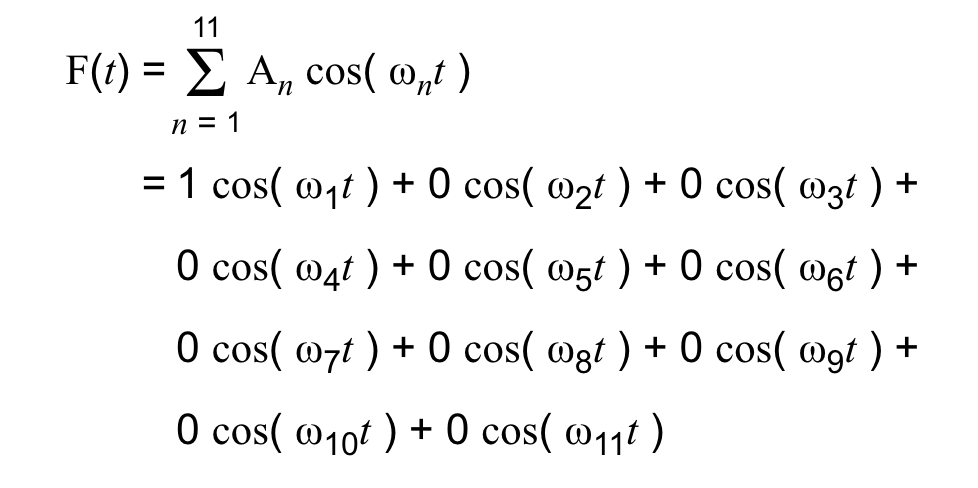
\includegraphics{/Users/kiloverse/Documents/物理学実験2/音のフーリエ解析/data/report_figs/cos展開式.png}}
          \caption{cos波の展開式[3]}
        \end{minipage}% % 在两个 minipage 环境之间使用 % 符号来消除之间的空白
        \begin{minipage}[b]{0.49\textwidth}
          \centering
          \adjustbox{height=0.18\textheight,keepaspectratio}{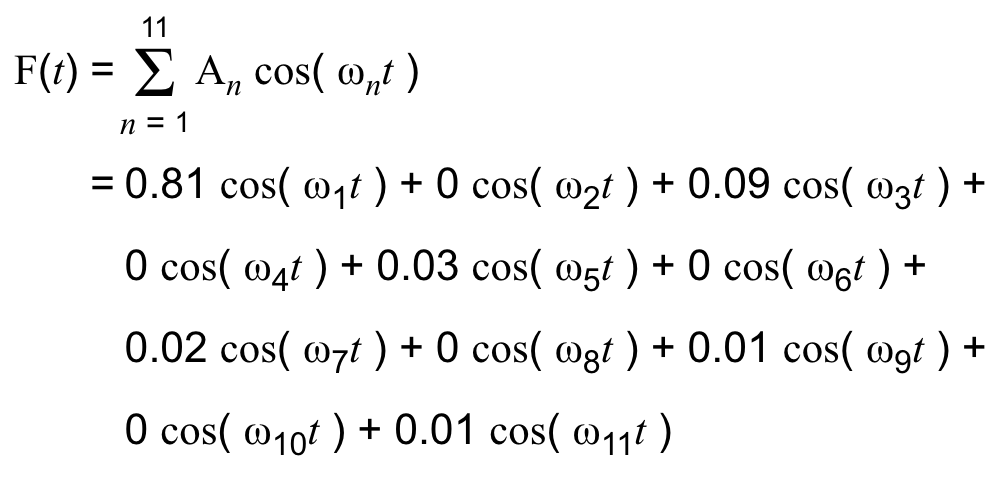
\includegraphics{/Users/kiloverse/Documents/物理学実験2/音のフーリエ解析/data/report_figs/三角展開式.png}}
          \caption{三角波の展開式[3]}
        \end{minipage}
    \end{figure}
    \begin{figure}[htbp]
        \centering
        \begin{minipage}[b]{0.49\textwidth} % minipage 环境用于在同一行内并排放置内容,[b] 参数表示底部对齐,{0.5\textwidth} 设置 minipage 的宽度为页面宽度的一半
          \centering
          \adjustbox{height=0.18\textheight,keepaspectratio}{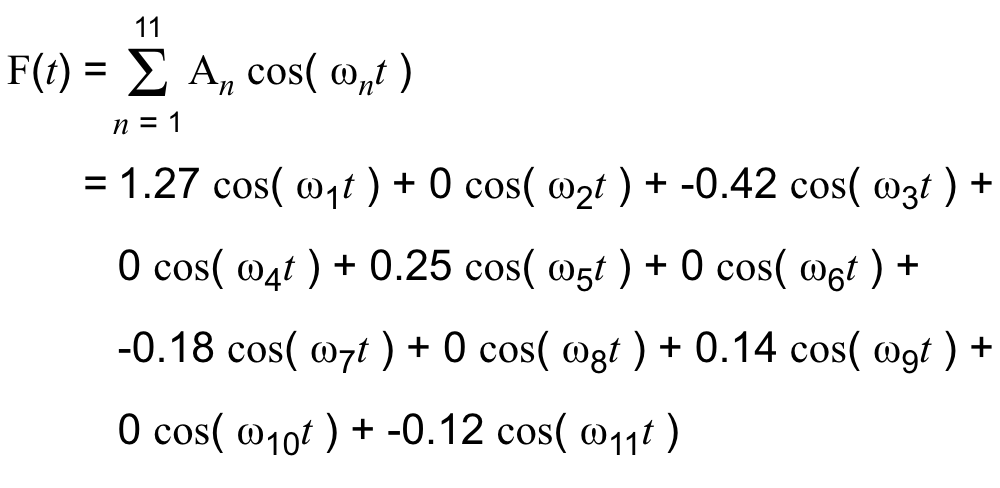
\includegraphics{/Users/kiloverse/Documents/物理学実験2/音のフーリエ解析/data/report_figs/矩形展開式.png}}
          \caption{矩形波の展開式[3]}
        \end{minipage}% % 在两个 minipage 环境之间使用 % 符号来消除之间的空白
        \begin{minipage}[b]{0.49\textwidth}
          \centering
          \adjustbox{height=0.17\textheight,keepaspectratio}{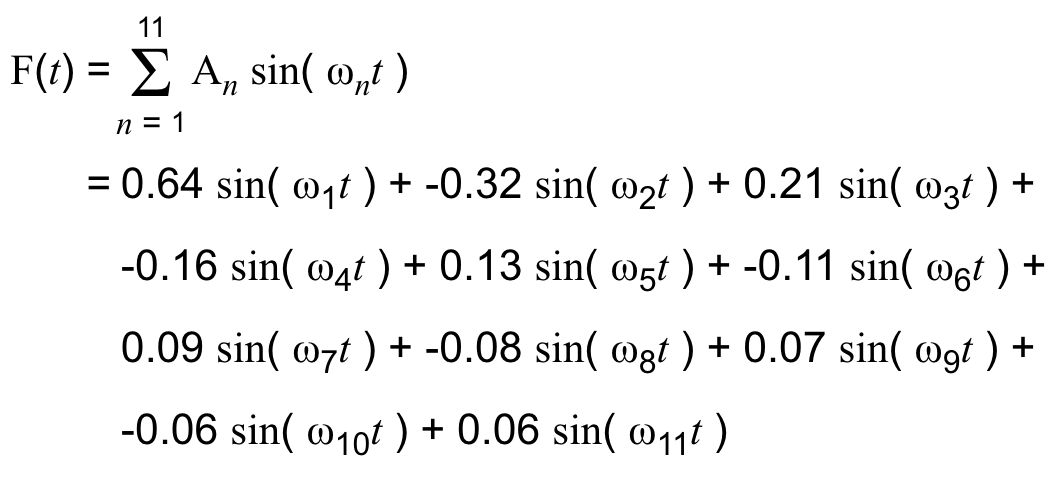
\includegraphics{/Users/kiloverse/Documents/物理学実験2/音のフーリエ解析/data/report_figs/鋸展開式.png}}
          \caption{鋸波の展開式[3]}
        \end{minipage}
    \end{figure}
    \FloatBarrier
    以上の展開によって、位相情報を落とした大きさだけの情報(展開係数$|C_n|$)が得られていることが確認できた。これは、元の波形から振幅情報のみを抽出し、各成分の周波数に対する影響の大きさを評価していることを意味している。この情報は多くの技術的応用に直接的な影響を与えており、位相情報が不要である場合には、計算の複雑さを軽減し、リアルタイム処理の高速化が可能になる。
\end{spacing}

\subsubsection{考察6:基底の取り方}
\begin{spacing}{1.2}
    \paragraph*{テキスト質問:}
    「Fourier Making Waves」ではsinとcosの2通りの基底の取り方が可能ですが、図に示された波形を再現するときにどのように選択したでしょうか?
    \paragraph*{解答:}
    テキストで示された図は偶関数のため、展開基底は同じく偶関数になっている$\cos(k_n t)$にするのが適切である。この場合、奇関数の$\sin$項の展開係数$b_n$はすべてゼロとなる。
    逆に、展開したい関数が奇関数の場合は、基底として$\sin$を選び、$\cos$項の係数$a_n$がゼロになる。
    フーリエ級数展開においては、対象とする波形の性質(偶関数性や奇関数性)に基づいて最も効率的な基底関数を選択することで、関数を正確に再現することが可能で、不要な係数が0になり、計算が単純化される。
\end{spacing}

\subsubsection{考察7:波形のずれ}
\begin{spacing}{1.2}
    図36と図37の矩形波と鋸波の波形図は、綺麗な矩形波や鋸波とはなっていない。その主な原因は展開項数の不足とAC結合(コンデンサを介した信号接続)にあると考察される。
    \subsubsection*{展開項数の影響}
    フーリエ級数展開の原理によると、展開係数が多いほど、関数と波形の近似が良くなる。このことを実際に目で見て確認するために、展開係数を色々変え、出力の結果を比較した。
    \begin{figure}[ht] % 选项 [htbp] 代表位置优先级, “here, top, bottom, page” 分别表示:此处、页顶、页底、单独一页
        \centering
        \fbox{\adjincludegraphics[width=0.8\textwidth]{/Users/kiloverse/Documents/物理学実験2/音のフーリエ解析/data/report_figs/違うnの矩形.png}}
        \caption{異なる展開係数nの矩形波形図}
    \end{figure}
    \begin{figure}[ht] % 选项 [htbp] 代表位置优先级, “here, top, bottom, page” 分别表示:此处、页顶、页底、单独一页
        \centering
        \fbox{\adjincludegraphics[width=0.8\textwidth]{/Users/kiloverse/Documents/物理学実験2/音のフーリエ解析/data/report_figs/違うnの鋸形.png}}
        \caption{異なる展開係数nの鋸形波形図}
    \end{figure}
    \FloatBarrier
    以上の結果から、展開係数が増加するに従って、波形上の細部が細かくなり、近似が良くなっていることが示されている。
    \vspace{50pt} % 每行大约12pt
    \subsubsection*{AC結合によるサグの発生}
    矩形図で観察できたように、波形の水平部分が斜めに見える「サグ」が観察された。
    \begin{figure}[ht] % 选项 [htbp] 代表位置优先级, “here, top, bottom, page” 分别表示:此处、页顶、页底、单独一页
        \centering
        \fbox{\adjincludegraphics[width=0.7\textwidth]{/Users/kiloverse/Documents/物理学実験2/音のフーリエ解析/data/result_plot/3_osc_squ.png}}
        \caption{矩形の波形図のサグ}
    \end{figure}
    \FloatBarrier
    この「サグ」はコンデンサと抵抗によるハイパスフィルタによって形成されたと考察される。

    コンデンサの基本的な性質により、直流電流は流れず、高い周波数の交流信号ほど電流が流れやすくなる。この性質を利用して、コンデンサと抵抗を組み合わせることで、不要な周波数の信号を減衰させ、必要な周波数の信号を通過させるフィルタ回路を構成することができる。
    \begin{figure}[ht] % 选项 [htbp] 代表位置优先级, “here, top, bottom, page” 分别表示:此处、页顶、页底、单独一页
        \centering
        \fbox{\adjincludegraphics[width=0.4\textwidth]{/Users/kiloverse/Documents/物理学実験2/音のフーリエ解析/data/report_figs/ハイパスフィルタ回路.png}}
        \caption{ハイパスフィルタ回路[13]}
    \end{figure}
    \FloatBarrier
    上図の回路は低い周波数の信号を減衰させ、高い周波数成分だけを通過させるハイパスフィルタである。信号を減衰させるか通過させるかの境界の周波数のことをカットオフ周波数と呼ぶ[13]。
    カットオフ周波数近くの信号を入力した場合、その波形が正弦波か矩形波かによって、入出力間の波形の変化が大きく異なる。正弦波を入力した場合、出力信号も正弦波であるが、矩形波を入力した場合、出力信号は入力信号のエッジ部分を取り出した波形になるという特性がある。
    \begin{figure}[ht] % 选项 [htbp] 代表位置优先级, “here, top, bottom, page” 分别表示:此处、页顶、页底、单独一页
        \centering
        \fbox{\adjincludegraphics[width=0.7\textwidth]{/Users/kiloverse/Documents/物理学実験2/音のフーリエ解析/data/report_figs/矩形の出力波形と入力波形の比較.png}}
        \caption{矩形の出力波形と入力波形の比較[13]}
    \end{figure}
    \FloatBarrier
    以上のことから、矩形波の波形図にサグ現象が起こったのは、ノイズ処理の過程で、AC結合によって形成されたと考察される。
\end{spacing}

\newpage
\subsubsection{課題3-2:波形を再現する一般的な指針}
\begin{spacing}{1.2}
    Fourier Making Wavesサイト[3]には、与えられた合成波の波形にぴったり合わせるための展開係数を調整するゲームがある。自分は様々な調整を試み、最も難しいLevel5の波形に対する11個の係数を特定することができた。
    \begin{figure}[ht] % 选项 [htbp] 代表位置优先级, “here, top, bottom, page” 分别表示:此处、页顶、页底、单独一页
        \centering
        \fbox{\adjincludegraphics[width=0.7\textwidth]{/Users/kiloverse/Documents/物理学実験2/音のフーリエ解析/data/report_figs/Level 5 を再現される係数.png}}
        \caption{Level 5 を再現される係数}
    \end{figure}
    \FloatBarrier
    以下に、この波形を再現するゲームについての一般的な指針をまとめた:
    \begin{enumerate}[label=\arabic*), before=\begin{spacing}{1.2}, after=\end{spacing}] % \arabic阿拉伯数字,\roman小写罗马数字,\Roman,\alph小写字母,\Alph,“*”之后添加自己喜欢的序号后样式, 如1.添加“.”,1)添加“)”;利用{spacing}自定义\item内的行间距
        \item まず、展開項の節を観察し、もし特定の展開項以外に他の展開項がその節になる場合、その展開項の係数を直接に特定できるので、この点を適切に利用する。
        \item 次に、振幅については気にせず、とりあえず係数を色々調整し、増減性が同じである合成波を作成する。
        \item 増減性が同じである合成波を得た後、波の全体的な位置はnが小さいときの係数に大きく依存しているため、この点を利用してnが小さいときの係数の大きさを大まかに特定する。
        \item 脳内に波形全体の誤差関数を把握し、全体的な誤差が最小になるように少しずつ係数を調整し、波形を再現できるまで続ける。
    \end{enumerate}
\end{spacing}

\newpage
\subsection{実験4:弦の振動}
\subsubsection{実験4結果}
\begin{spacing}{1.2}
    まず、ギターの普通奏法において、弦の中心部を押して弾くと、周波数分布の結果は以下となった:
    \begin{figure}[ht] % 选项 [htbp] 代表位置优先级, “here, top, bottom, page” 分别表示:此处、页顶、页底、单独一页
        \centering
        \fbox{\adjincludegraphics[width=0.9\textwidth]{/Users/kiloverse/Documents/物理学実験2/音のフーリエ解析/data/result_plot/4_fft_mid.png}}
        \caption{ギターの中心部を押して弾いた結果}
    \end{figure}
    \FloatBarrier
    弦の中心部を押して弾いた場合、奇数次モードの振動が主に励起され、基本周波数と低次のハーモニクスが顕著に現れた。

    また、何もしなくて、ブリッジの周りを弾くと、結果は以下となった:
    \begin{figure}[ht] % 选项 [htbp] 代表位置优先级, “here, top, bottom, page” 分别表示:此处、页顶、页底、单独一页
        \centering
        \fbox{\adjincludegraphics[width=0.9\textwidth]{/Users/kiloverse/Documents/物理学実験2/音のフーリエ解析/data/result_plot/4_fft_end.png}}
        \caption{ギターのブリッジ付近を弾いた結果}
    \end{figure}
    \FloatBarrier
    何もしなくて、ブリッジの周りを弾いた場合、複雑な振動モードが励起され、多くの高次ハーモニクスが生成された。
    \newpage
    次に、弦の1/nの位置を軽く触れながら弾くと、ハーモニックス奏法というものになって、周波数分布の結果は、下図のように、n倍振動のところだけに1本のピークが現れた。
    \begin{figure}[htbp]
        \centering
        \begin{minipage}[b]{0.49\textwidth} % minipage 环境用于在同一行内并排放置内容,[b] 参数表示底部对齐,{0.5\textwidth} 设置 minipage 的宽度为页面宽度的一半
          \centering
          \fbox{\adjustbox{height=0.3\textheight,keepaspectratio}{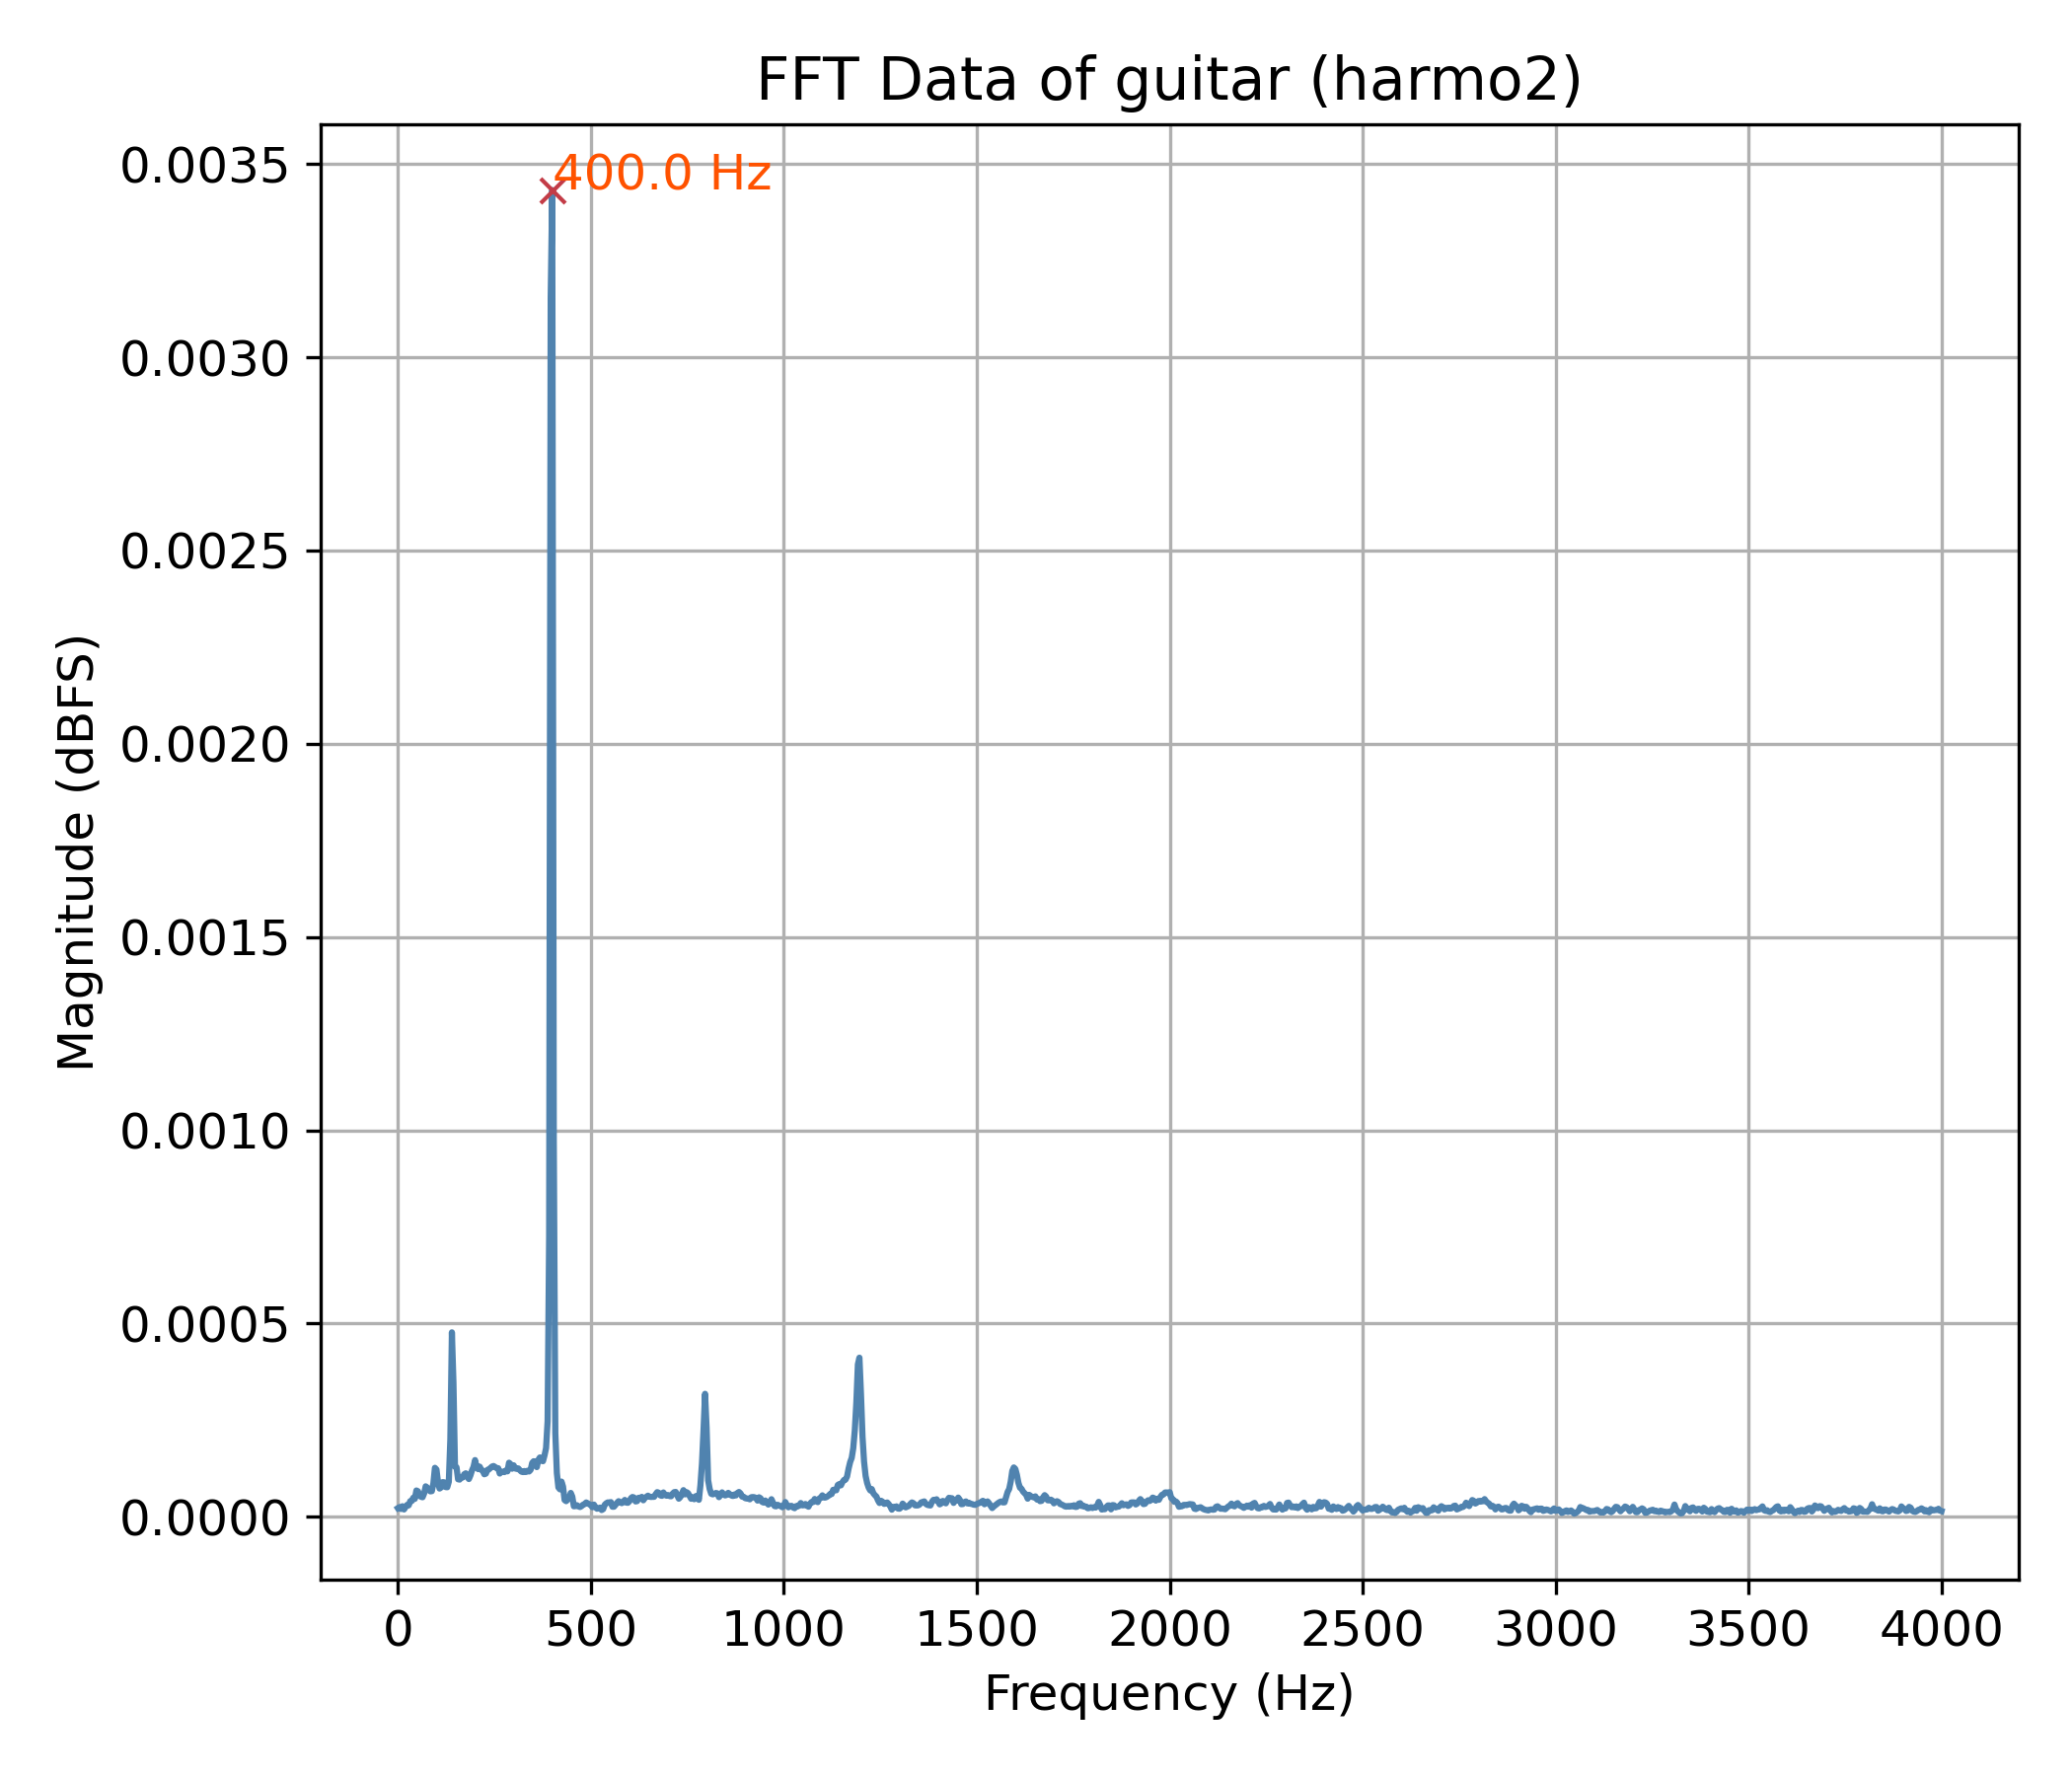
\includegraphics{/Users/kiloverse/Documents/物理学実験2/音のフーリエ解析/data/result_plot/4_fft_harmo2.png}}}
          \caption{弦の1/2のところを触れた結果}
        \end{minipage}% % 在两个 minipage 环境之间使用 % 符号来消除之间的空白
        \begin{minipage}[b]{0.49\textwidth}
          \centering
          \fbox{\adjustbox{height=0.3\textheight,keepaspectratio}{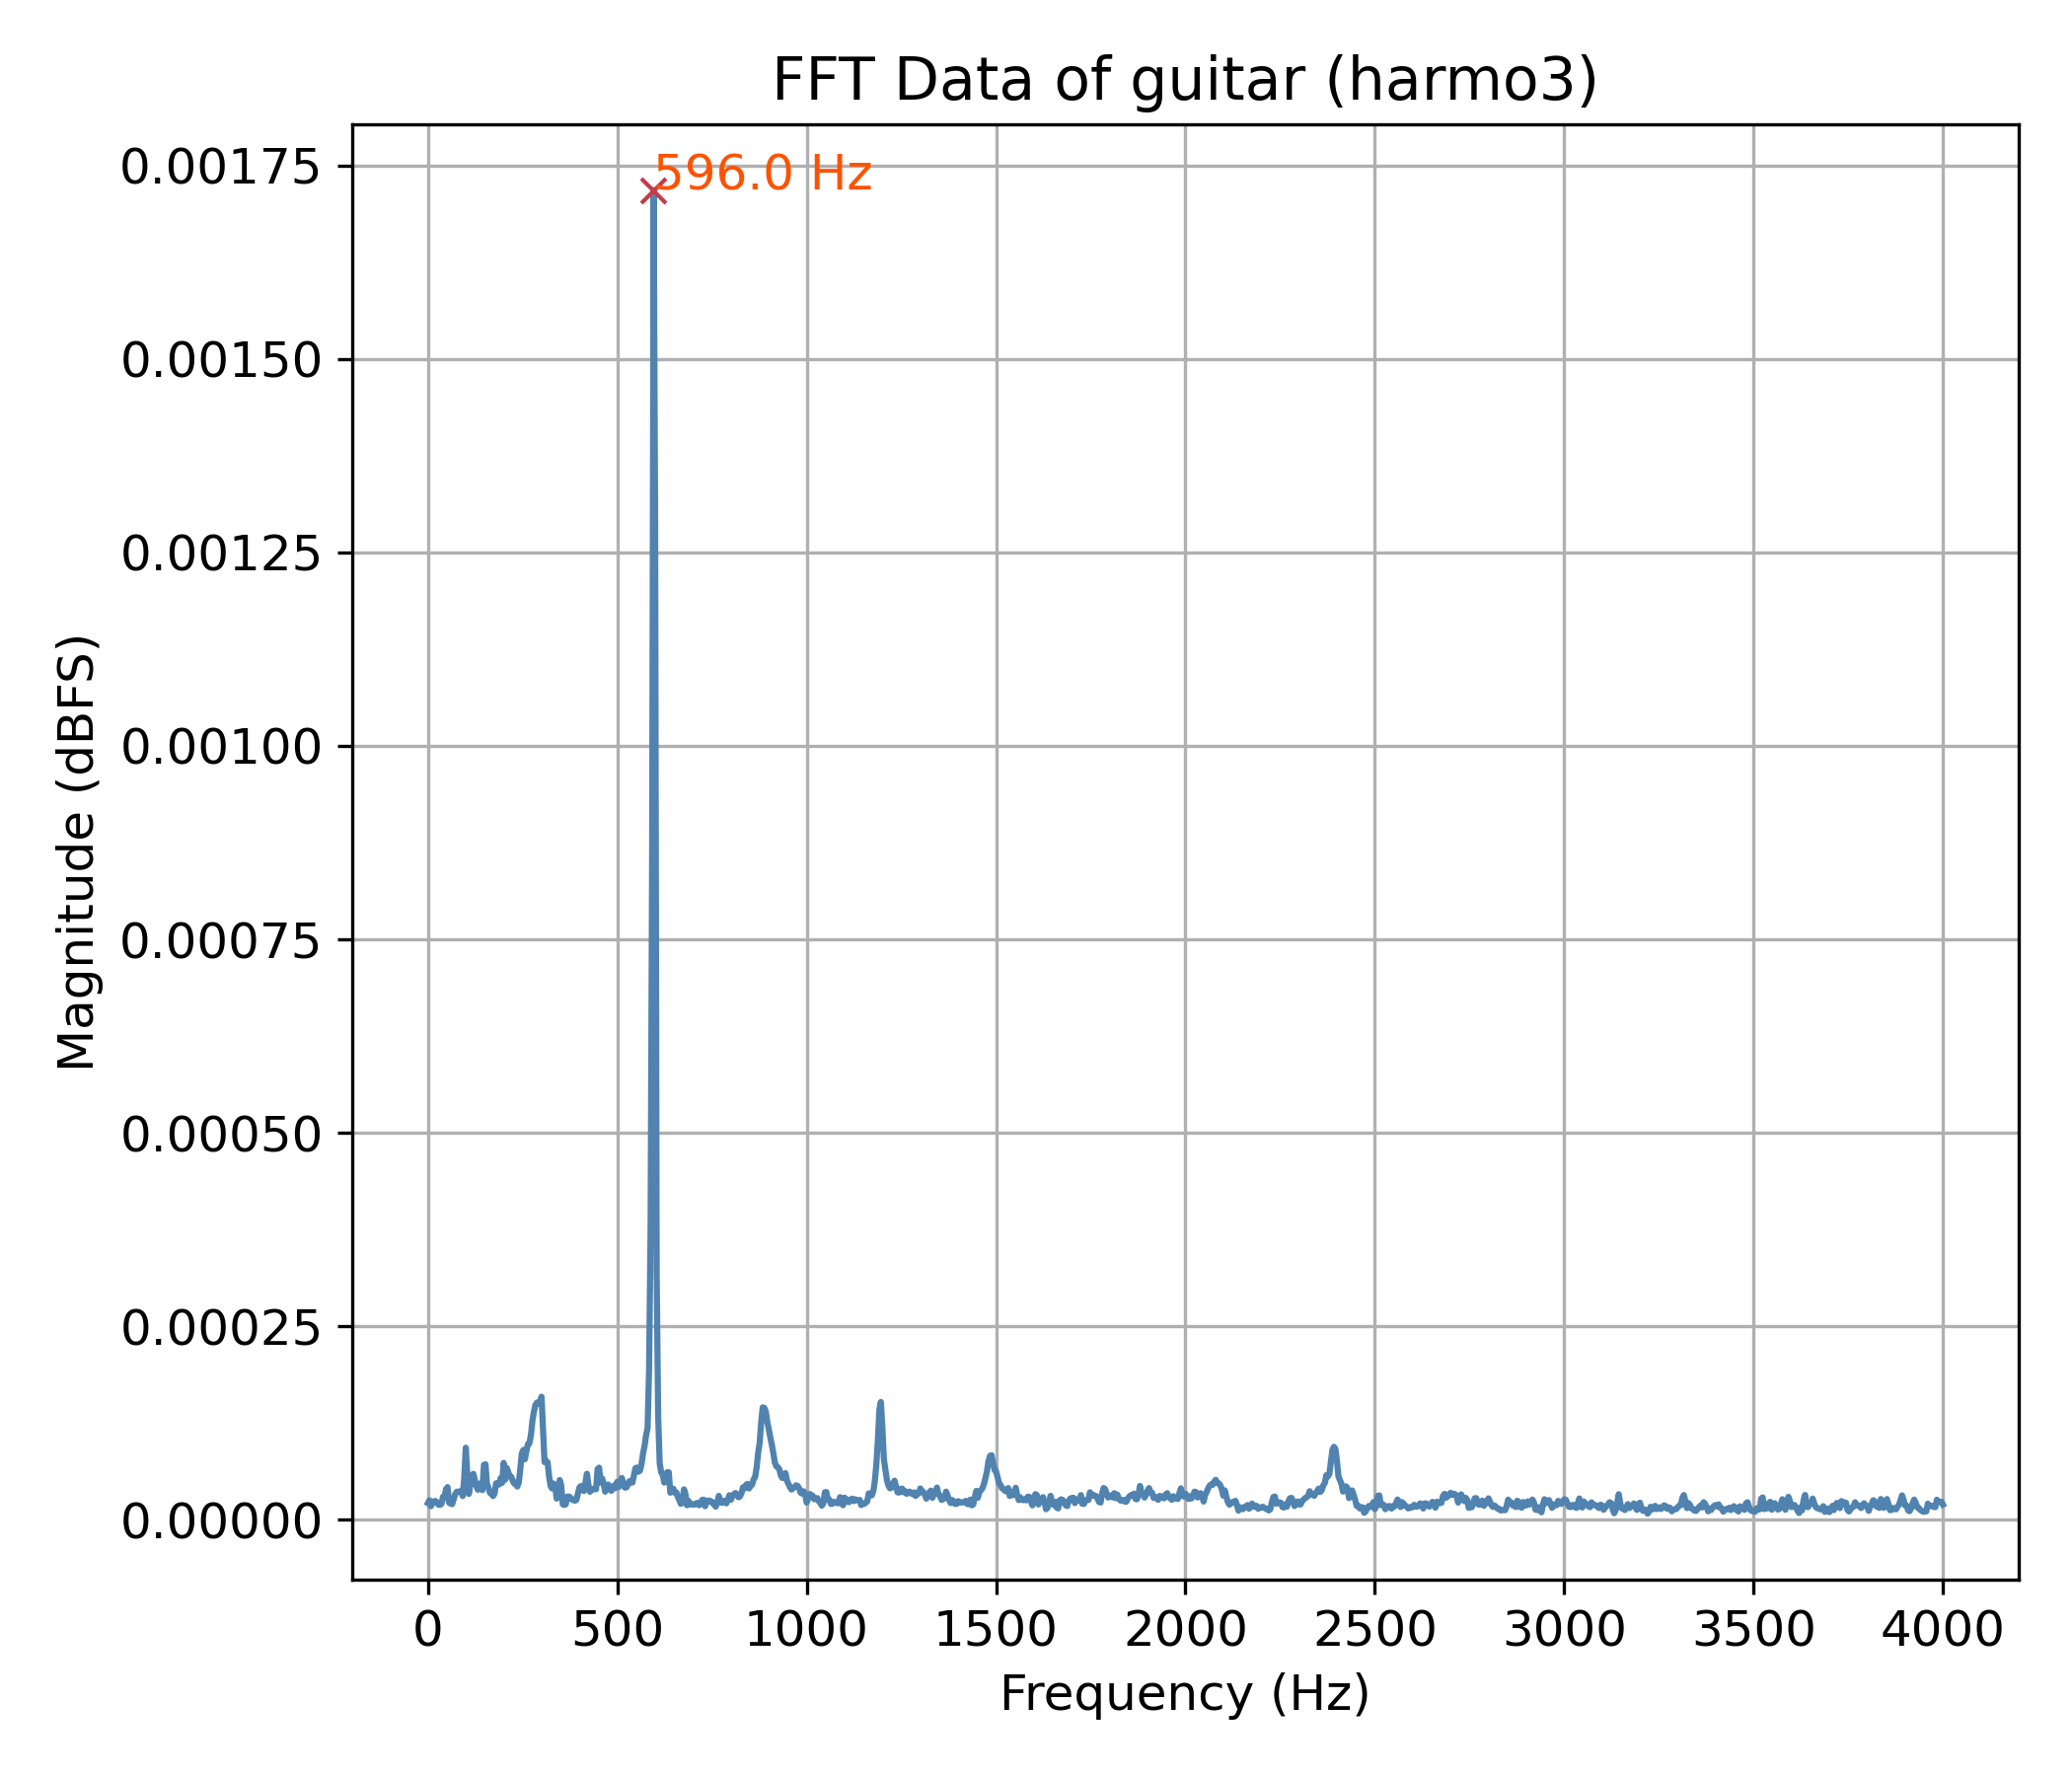
\includegraphics{/Users/kiloverse/Documents/物理学実験2/音のフーリエ解析/data/result_plot/4_fft_harmo3.png}}}
          \caption{弦の1/3のところを触れた結果}
        \end{minipage}
    \end{figure}
    \begin{figure}[htbp]
        \centering
        \begin{minipage}[b]{0.49\textwidth} % minipage 环境用于在同一行内并排放置内容,[b] 参数表示底部对齐,{0.5\textwidth} 设置 minipage 的宽度为页面宽度的一半
          \centering
          \fbox{\adjustbox{height=0.3\textheight,keepaspectratio}{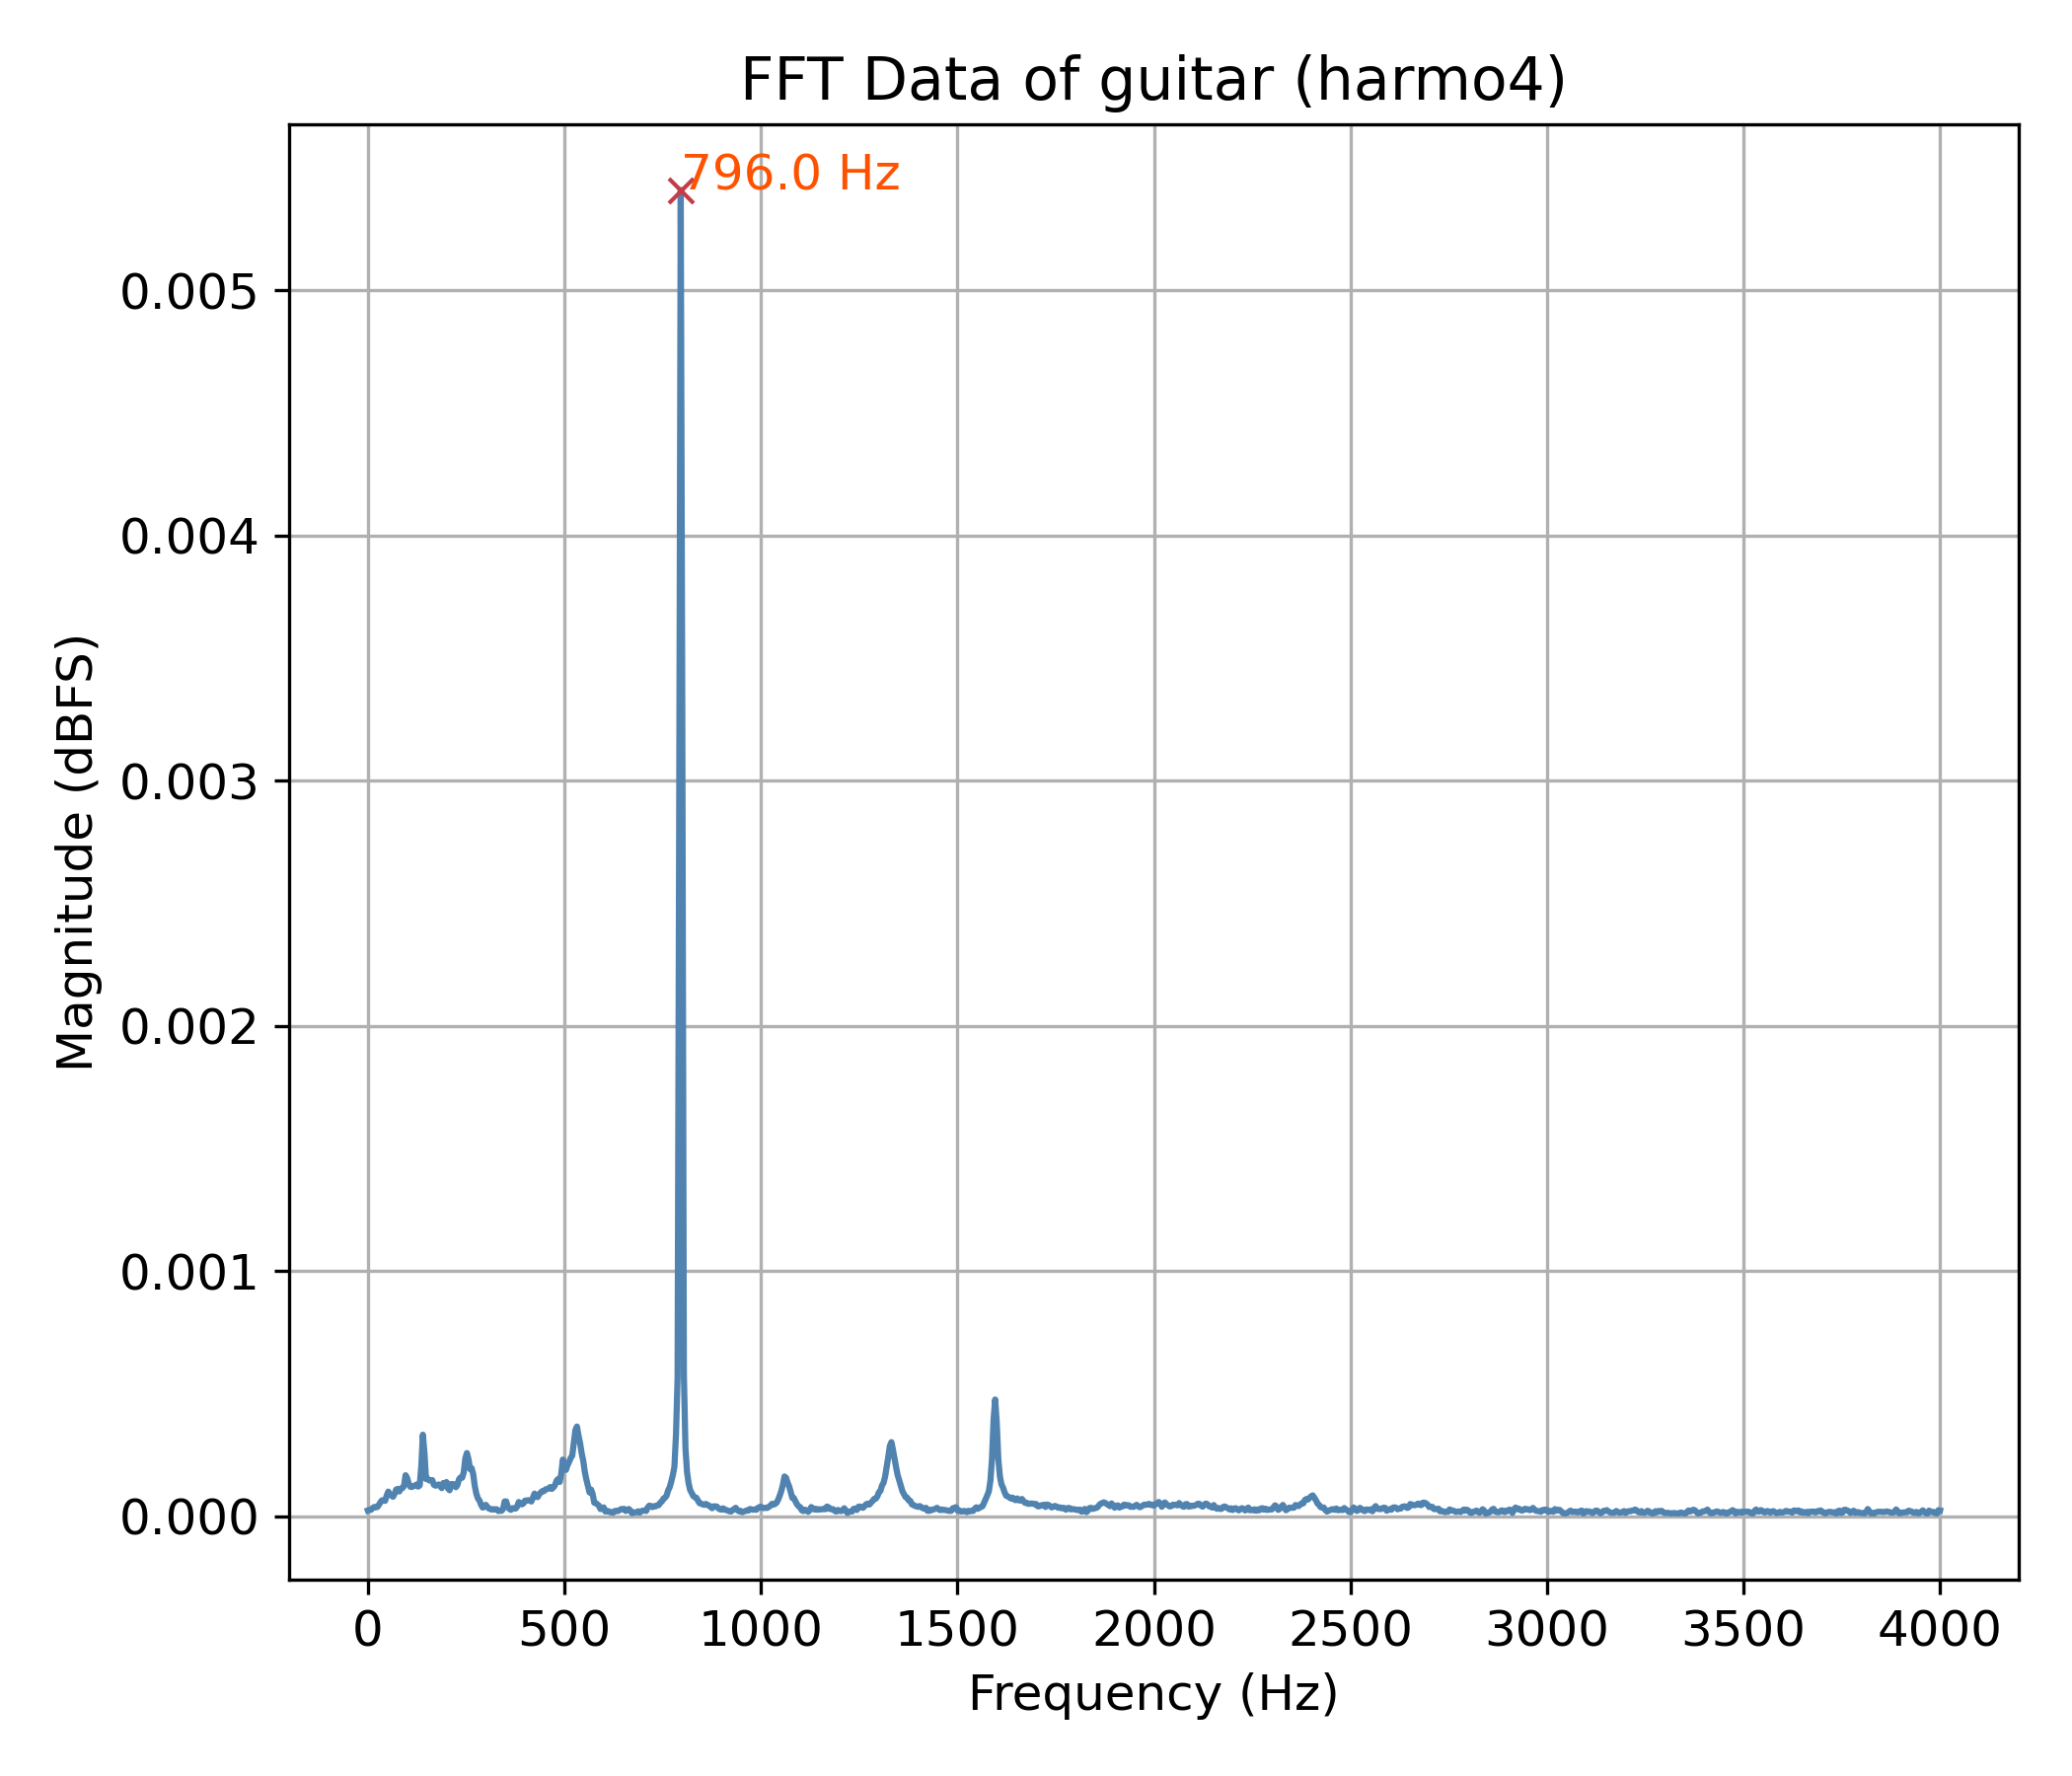
\includegraphics{/Users/kiloverse/Documents/物理学実験2/音のフーリエ解析/data/result_plot/4_fft_harmo4.png}}}
          \caption{弦の1/4のところを触れた結果}
        \end{minipage}% % 在两个 minipage 环境之间使用 % 符号来消除之间的空白
        \begin{minipage}[b]{0.49\textwidth}
          \centering
          \fbox{\adjustbox{height=0.3\textheight,keepaspectratio}{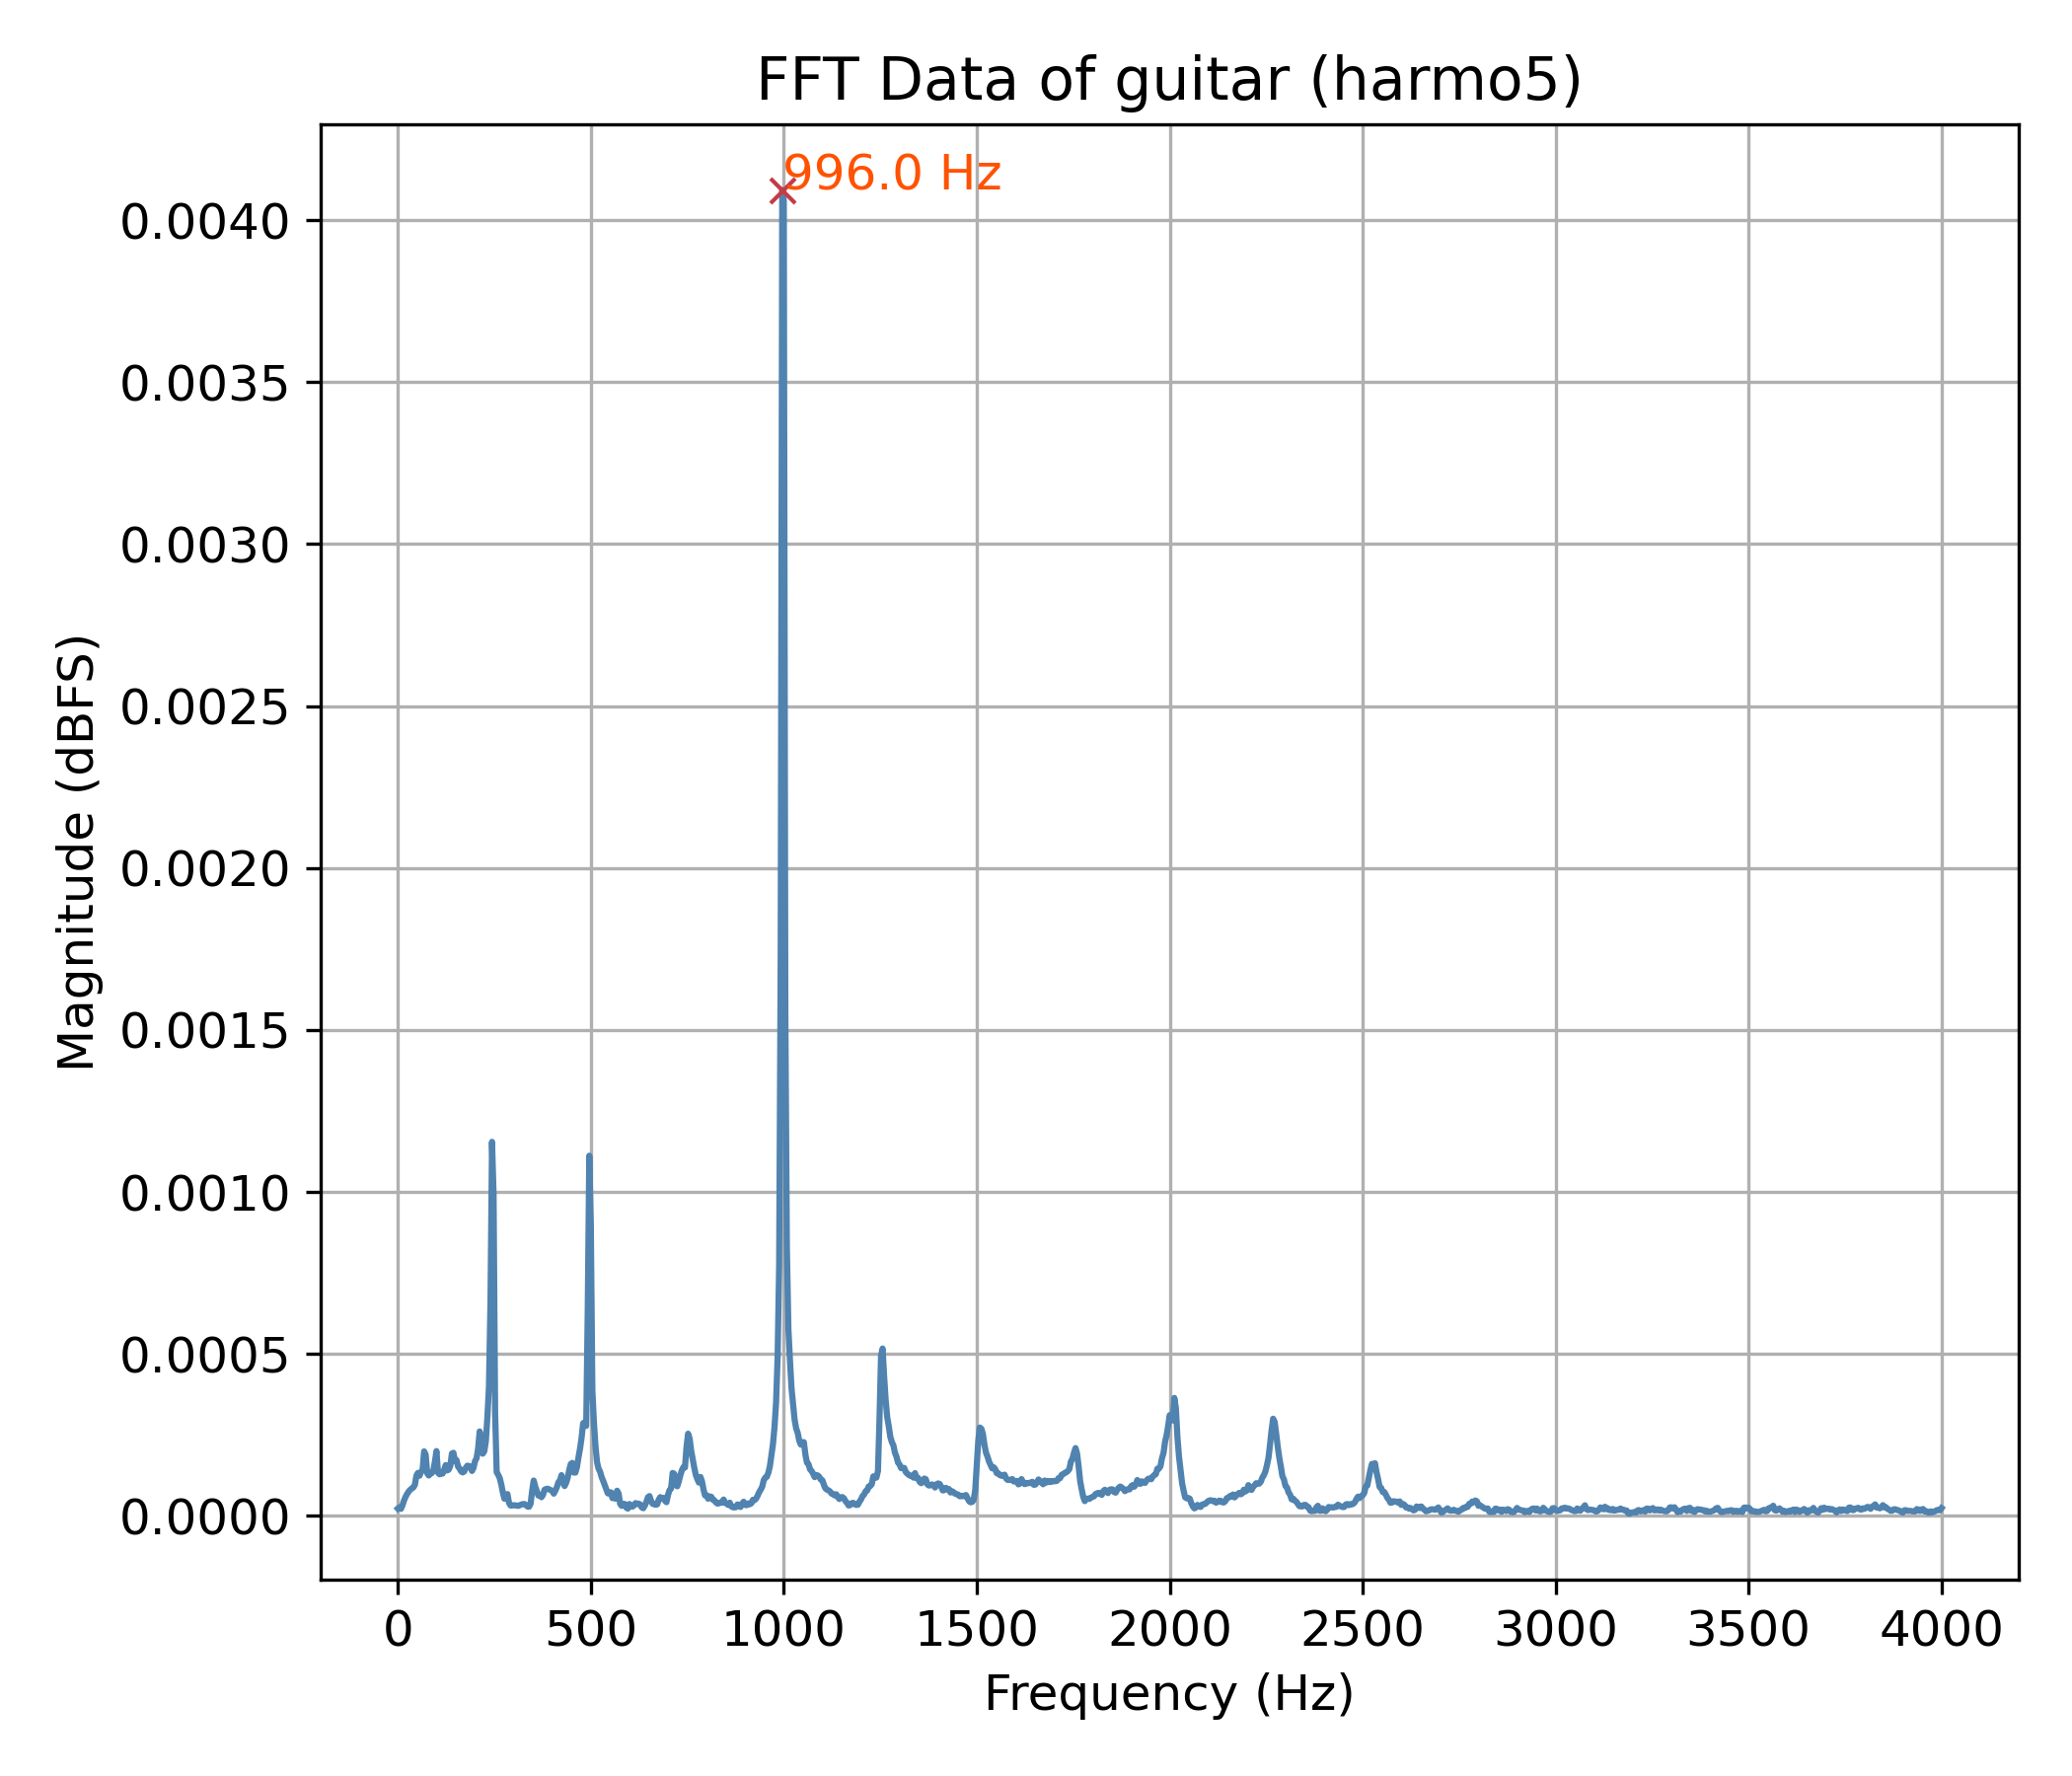
\includegraphics{/Users/kiloverse/Documents/物理学実験2/音のフーリエ解析/data/result_plot/4_fft_harmo5.png}}}
          \caption{弦の1/5のところを触れた結果}
        \end{minipage}
    \end{figure}
    \FloatBarrier
\end{spacing}

\newpage
\subsubsection{課題4-1:ハーモニックス奏法}
\begin{spacing}{1.2}
    「ハーモニックス」とは、ギターなどの弦楽器で一部のハーモニクス(倍音)を際立たせて音を鳴らす奏法である。この技術では、特定の点(通常、弦の長さの単純な分数点、例えば1/2、1/3、1/4など)で弦を軽く触れることにより、基本周波数の倍数であるハーモニクスを強調できる。

    ハーモニックスが強調される原因は、弦の特定の点(ノード)で弦を軽く触れると、その点で弦の振動がキャンセルされ、そこが節となり、n倍振動しか起こらないからである。たとえば、弦を中央で軽く触れると、弦はその長さの半分で振動し、基本周波数の2倍の周波数が生じる。このため、ハーモニックス奏法の周波数成分の図では、n倍振動の箇所にのみピークが現れる。
    \begin{figure}[htbp]
        \centering
        \begin{minipage}[b]{0.49\textwidth} % minipage 环境用于在同一行内并排放置内容,[b] 参数表示底部对齐,{0.5\textwidth} 设置 minipage 的宽度为页面宽度的一半
          \centering
          \adjustbox{height=0.07\textheight,keepaspectratio}{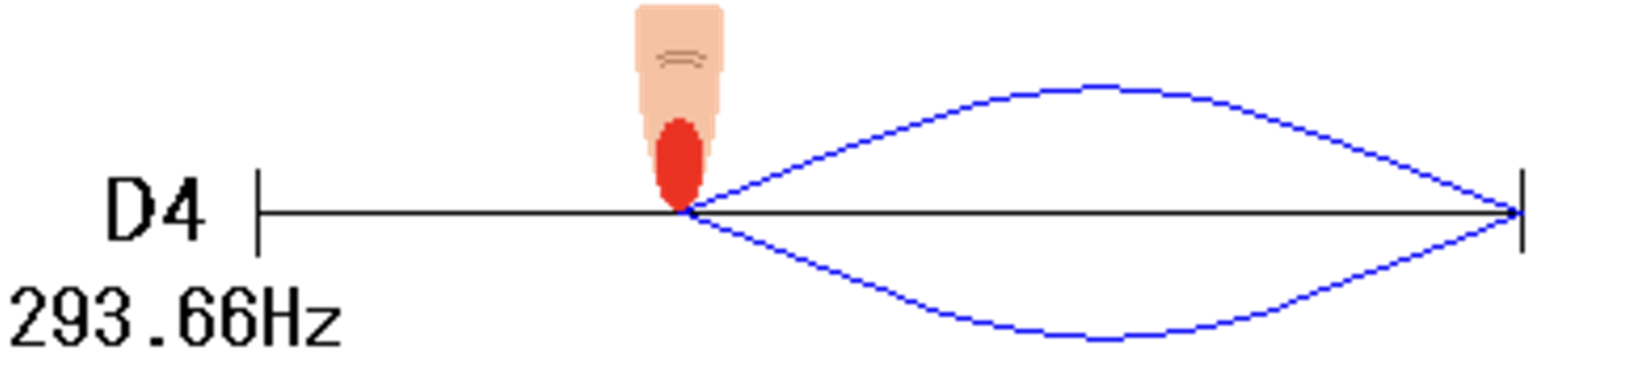
\includegraphics{/Users/kiloverse/Documents/物理学実験2/音のフーリエ解析/data/report_figs/普通奏法.png}}
          \caption{普通奏法[14]}
        \end{minipage}% % 在两个 minipage 环境之间使用 % 符号来消除之间的空白
        \begin{minipage}[b]{0.49\textwidth}
          \centering
          \adjustbox{height=0.075\textheight,keepaspectratio}{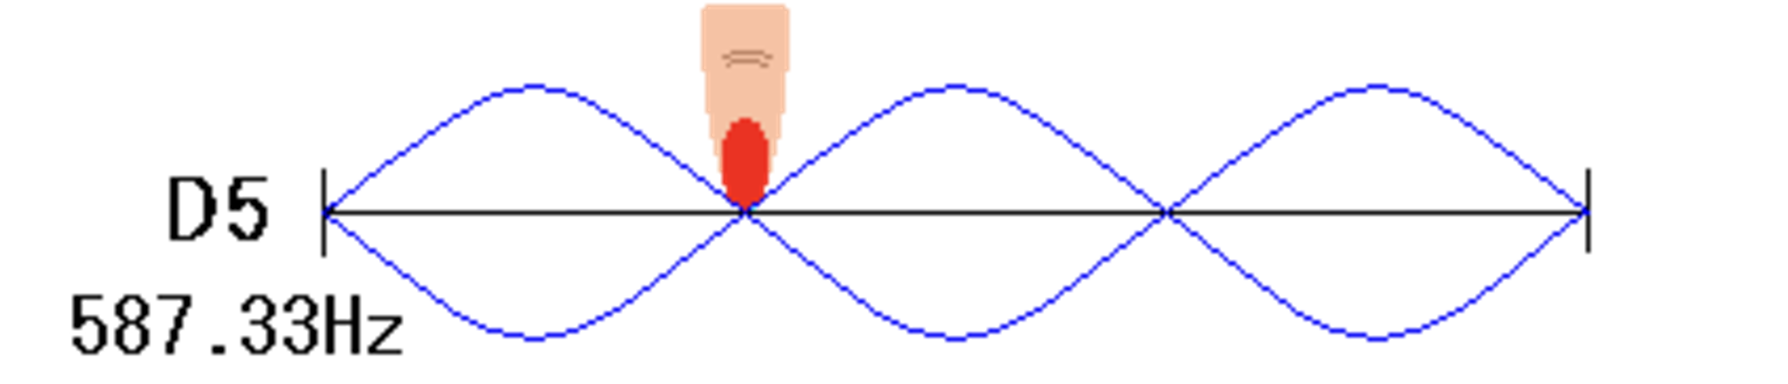
\includegraphics{/Users/kiloverse/Documents/物理学実験2/音のフーリエ解析/data/report_figs/ハーモニクス奏法.png}}
          \caption{ハーモニックス奏法[14]}
        \end{minipage}
    \end{figure}
    \FloatBarrier
    \subsubsection*{普通奏法とハーモニックス奏法の比較}
    普通奏法では、演奏者は指板上で弦を押さえることにより弦の有効長を短くし、その振動数は増加し、音の高さが上がる。この奏法では、押さえた位置によって弦の振動する部分の長さが決定され、それに応じて基本周波数が変化する。結果として、図50と図51のように、基本周波数と多くの倍音が混在するため、音色が豊かで暖かみがある。

    一方、ハーモニックス奏法では、弦の特定の点(例えば、弦の長さの1/2、1/3、1/4の位置など)を軽く触れることで、弦の振動を部分的に制限し、基本周波数の整数倍の周波数のみが強調される。この奏法によって生じる音は、特定の倍音のみが強調されるため、非常に純粋でクリーンな音が特徴である。ハーモニックスの音は、その独特の響きによって、音楽的なアクセントや効果を加えるのに用いられることが多い。
\end{spacing}

\subsubsection{課題4-2:様々な楽器の振動}
\begin{spacing}{1.2}
    ギター以外にも、さまざまな楽器の周波数成分について調べた。まず、木管楽器のパンパイプの周波数成分C6、D6、E6について、左図は通常のスケールで、右図はy軸をログスケールにしたものである。
    \begin{figure}[htbp]
        \centering
        \begin{minipage}[b]{0.49\textwidth} % minipage 环境用于在同一行内并排放置内容,[b] 参数表示底部对齐,{0.5\textwidth} 设置 minipage 的宽度为页面宽度的一半
          \centering
          \fbox{\adjustbox{height=0.265\textheight,keepaspectratio}{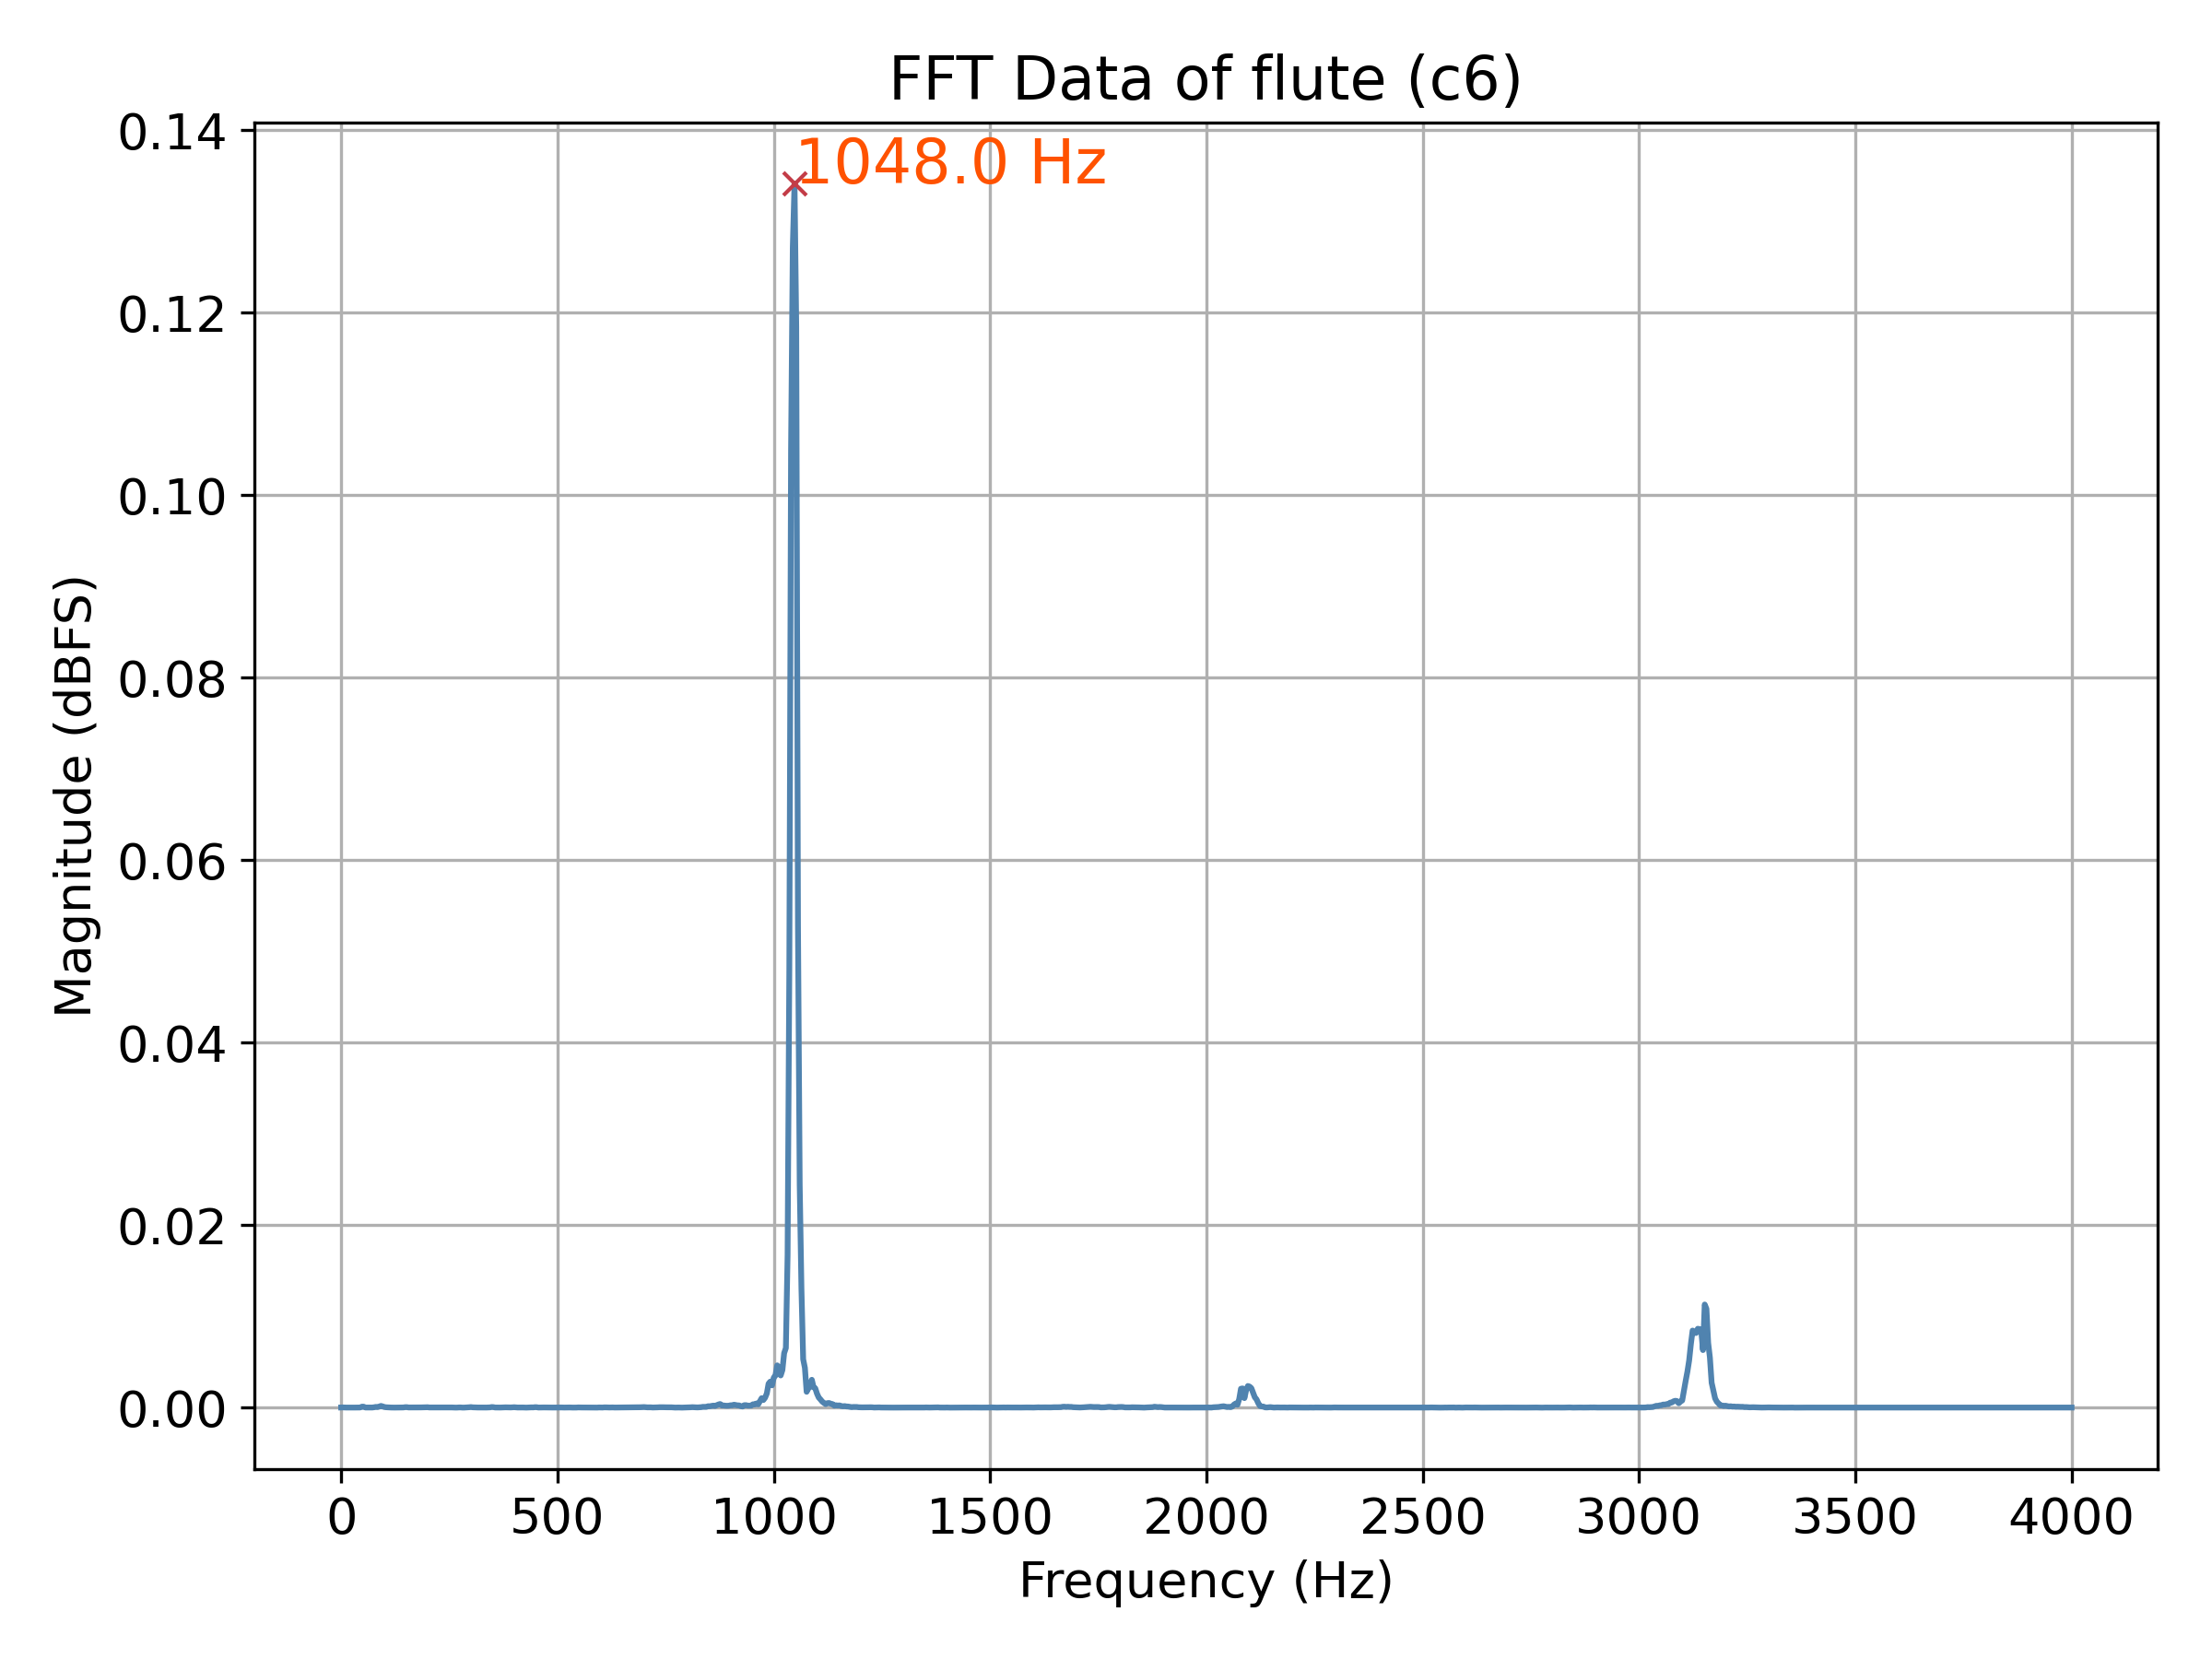
\includegraphics{/Users/kiloverse/Documents/物理学実験2/音のフーリエ解析/data/result_plot/4_fft_flute_c6.png}}}
          \caption{パンパイプC6音の周波数成分}
        \end{minipage}% % 在两个 minipage 环境之间使用 % 符号来消除之间的空白
        \begin{minipage}[b]{0.49\textwidth}
          \centering
          \fbox{\adjustbox{height=0.265\textheight,keepaspectratio}{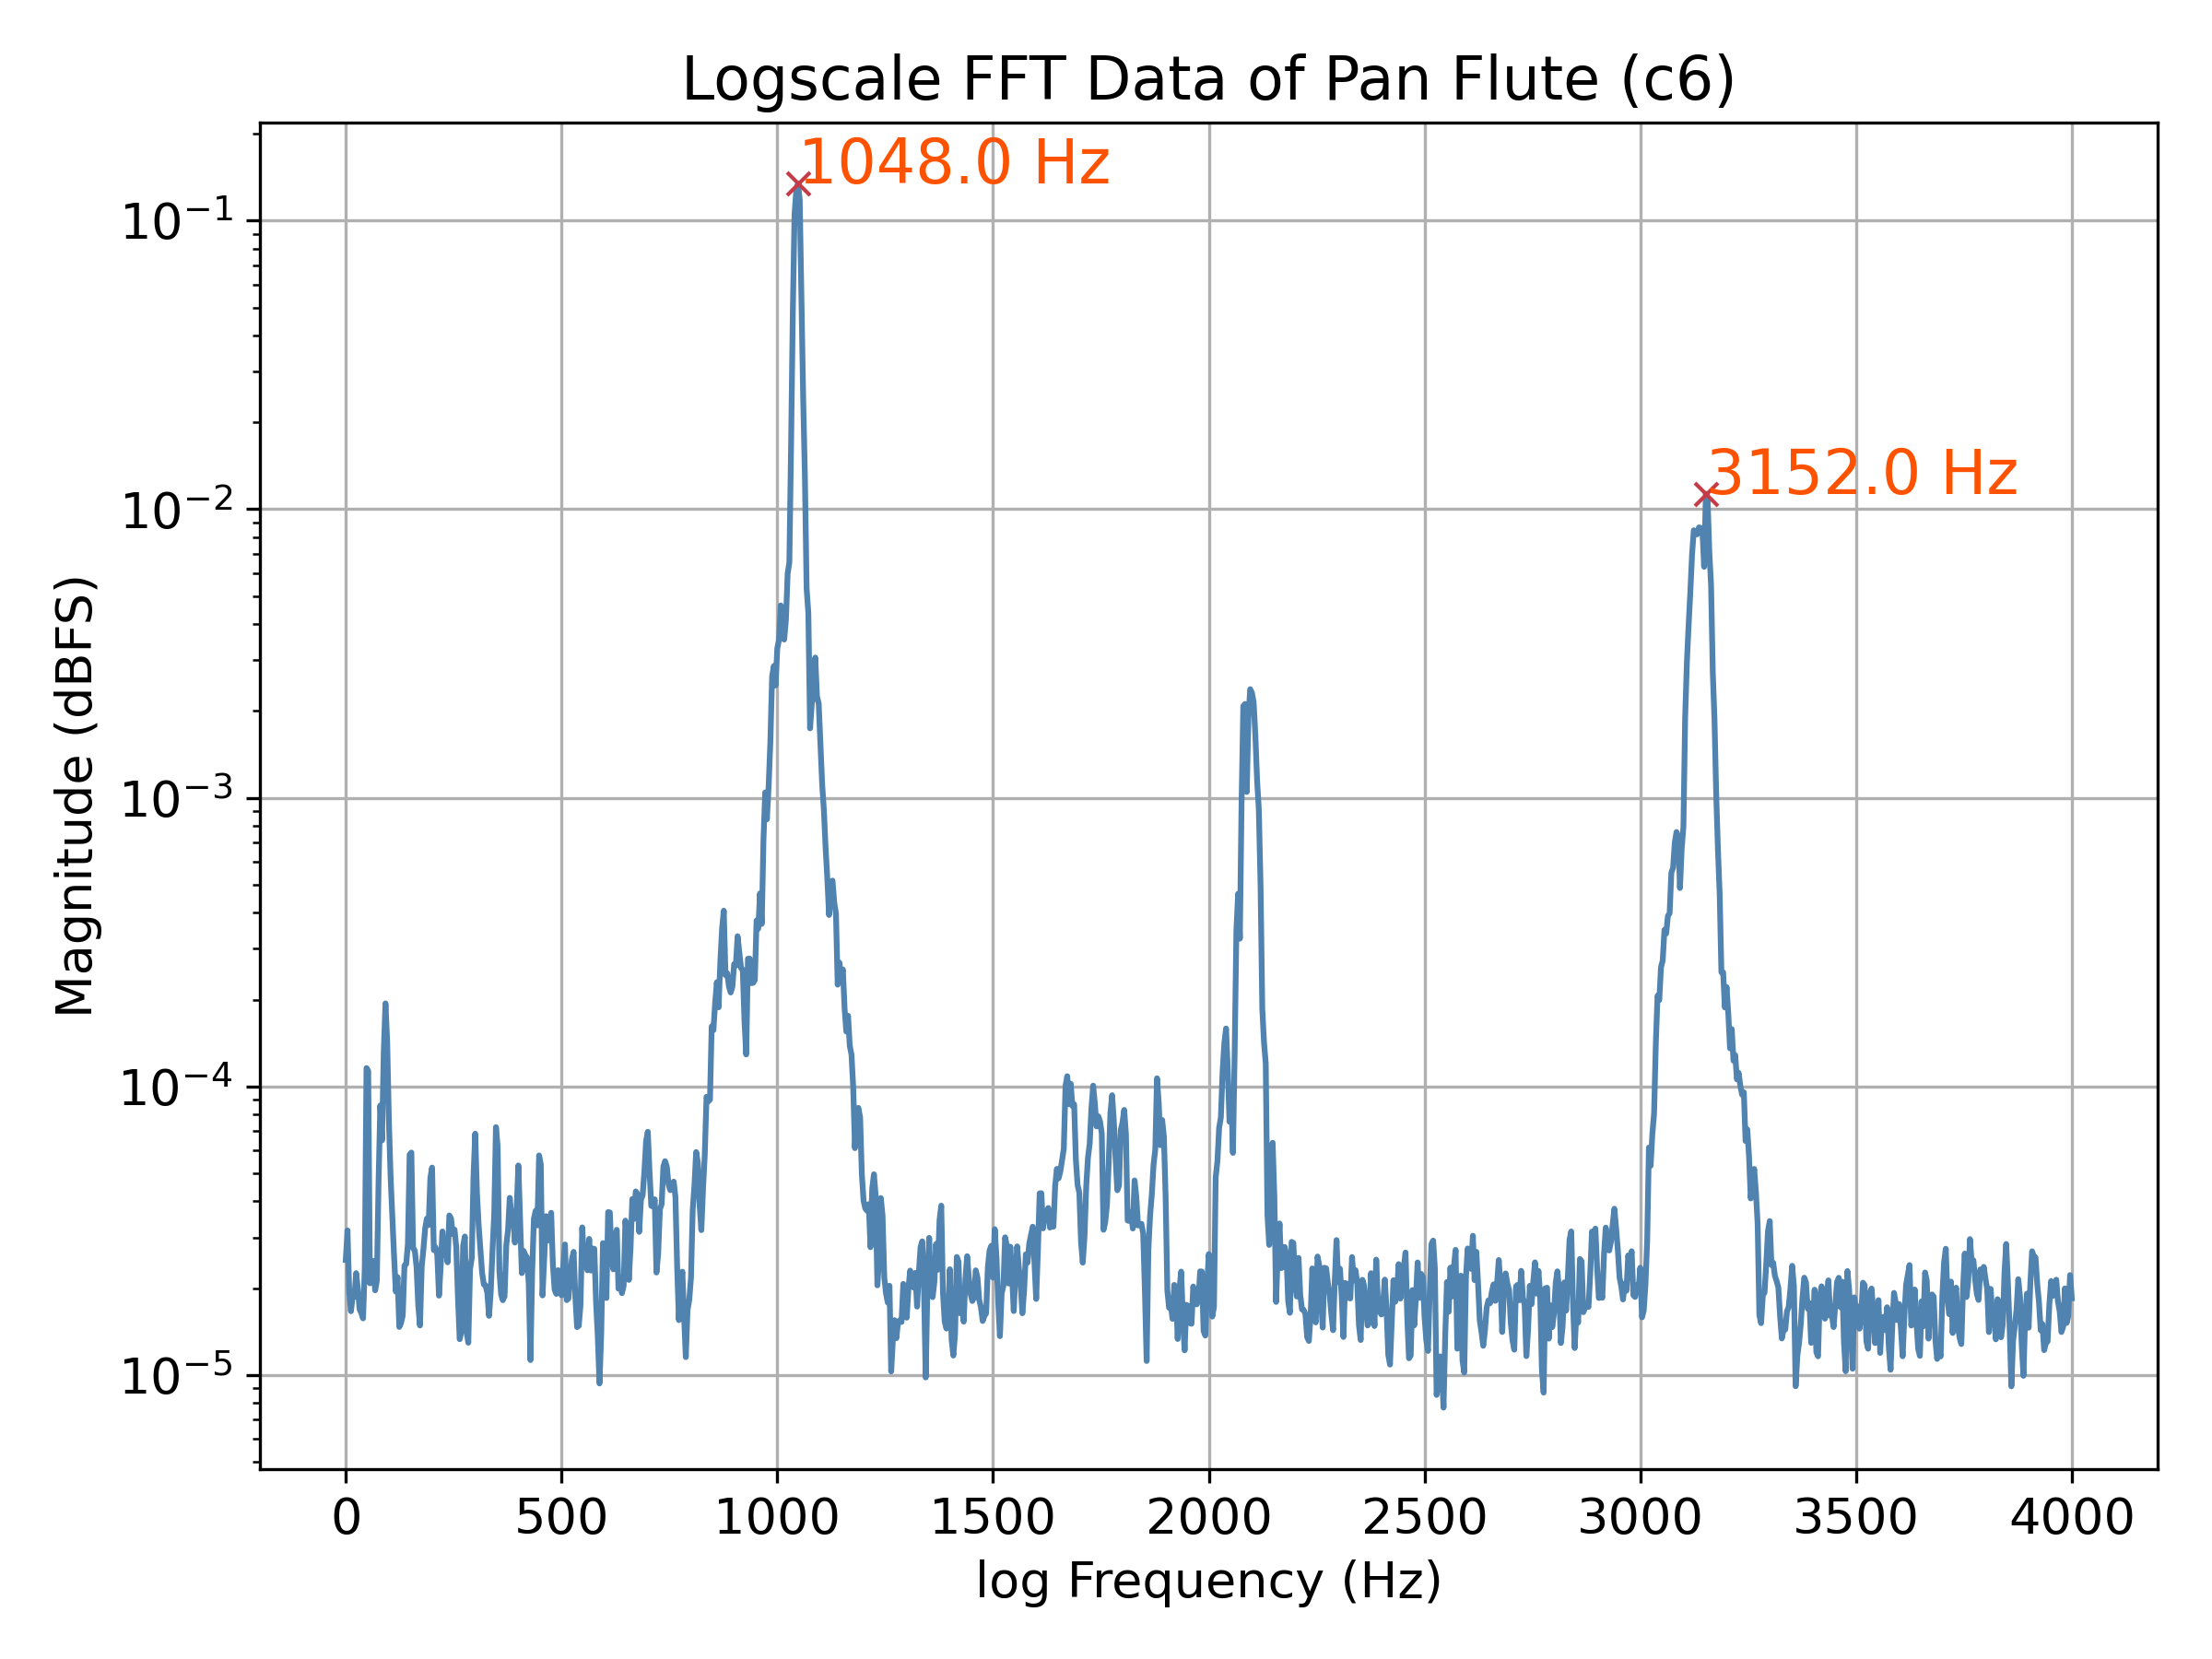
\includegraphics{/Users/kiloverse/Documents/物理学実験2/音のフーリエ解析/data/result_plot/4_fft_log_flute_c6.png}}}
          \caption{パンパイプC6音の周波数成分(y in logscale)}
        \end{minipage}
    \end{figure}
    \begin{figure}[htbp]
        \centering
        \begin{minipage}[b]{0.49\textwidth} % minipage 环境用于在同一行内并排放置内容,[b] 参数表示底部对齐,{0.5\textwidth} 设置 minipage 的宽度为页面宽度的一半
          \centering
          \fbox{\adjustbox{height=0.265\textheight,keepaspectratio}{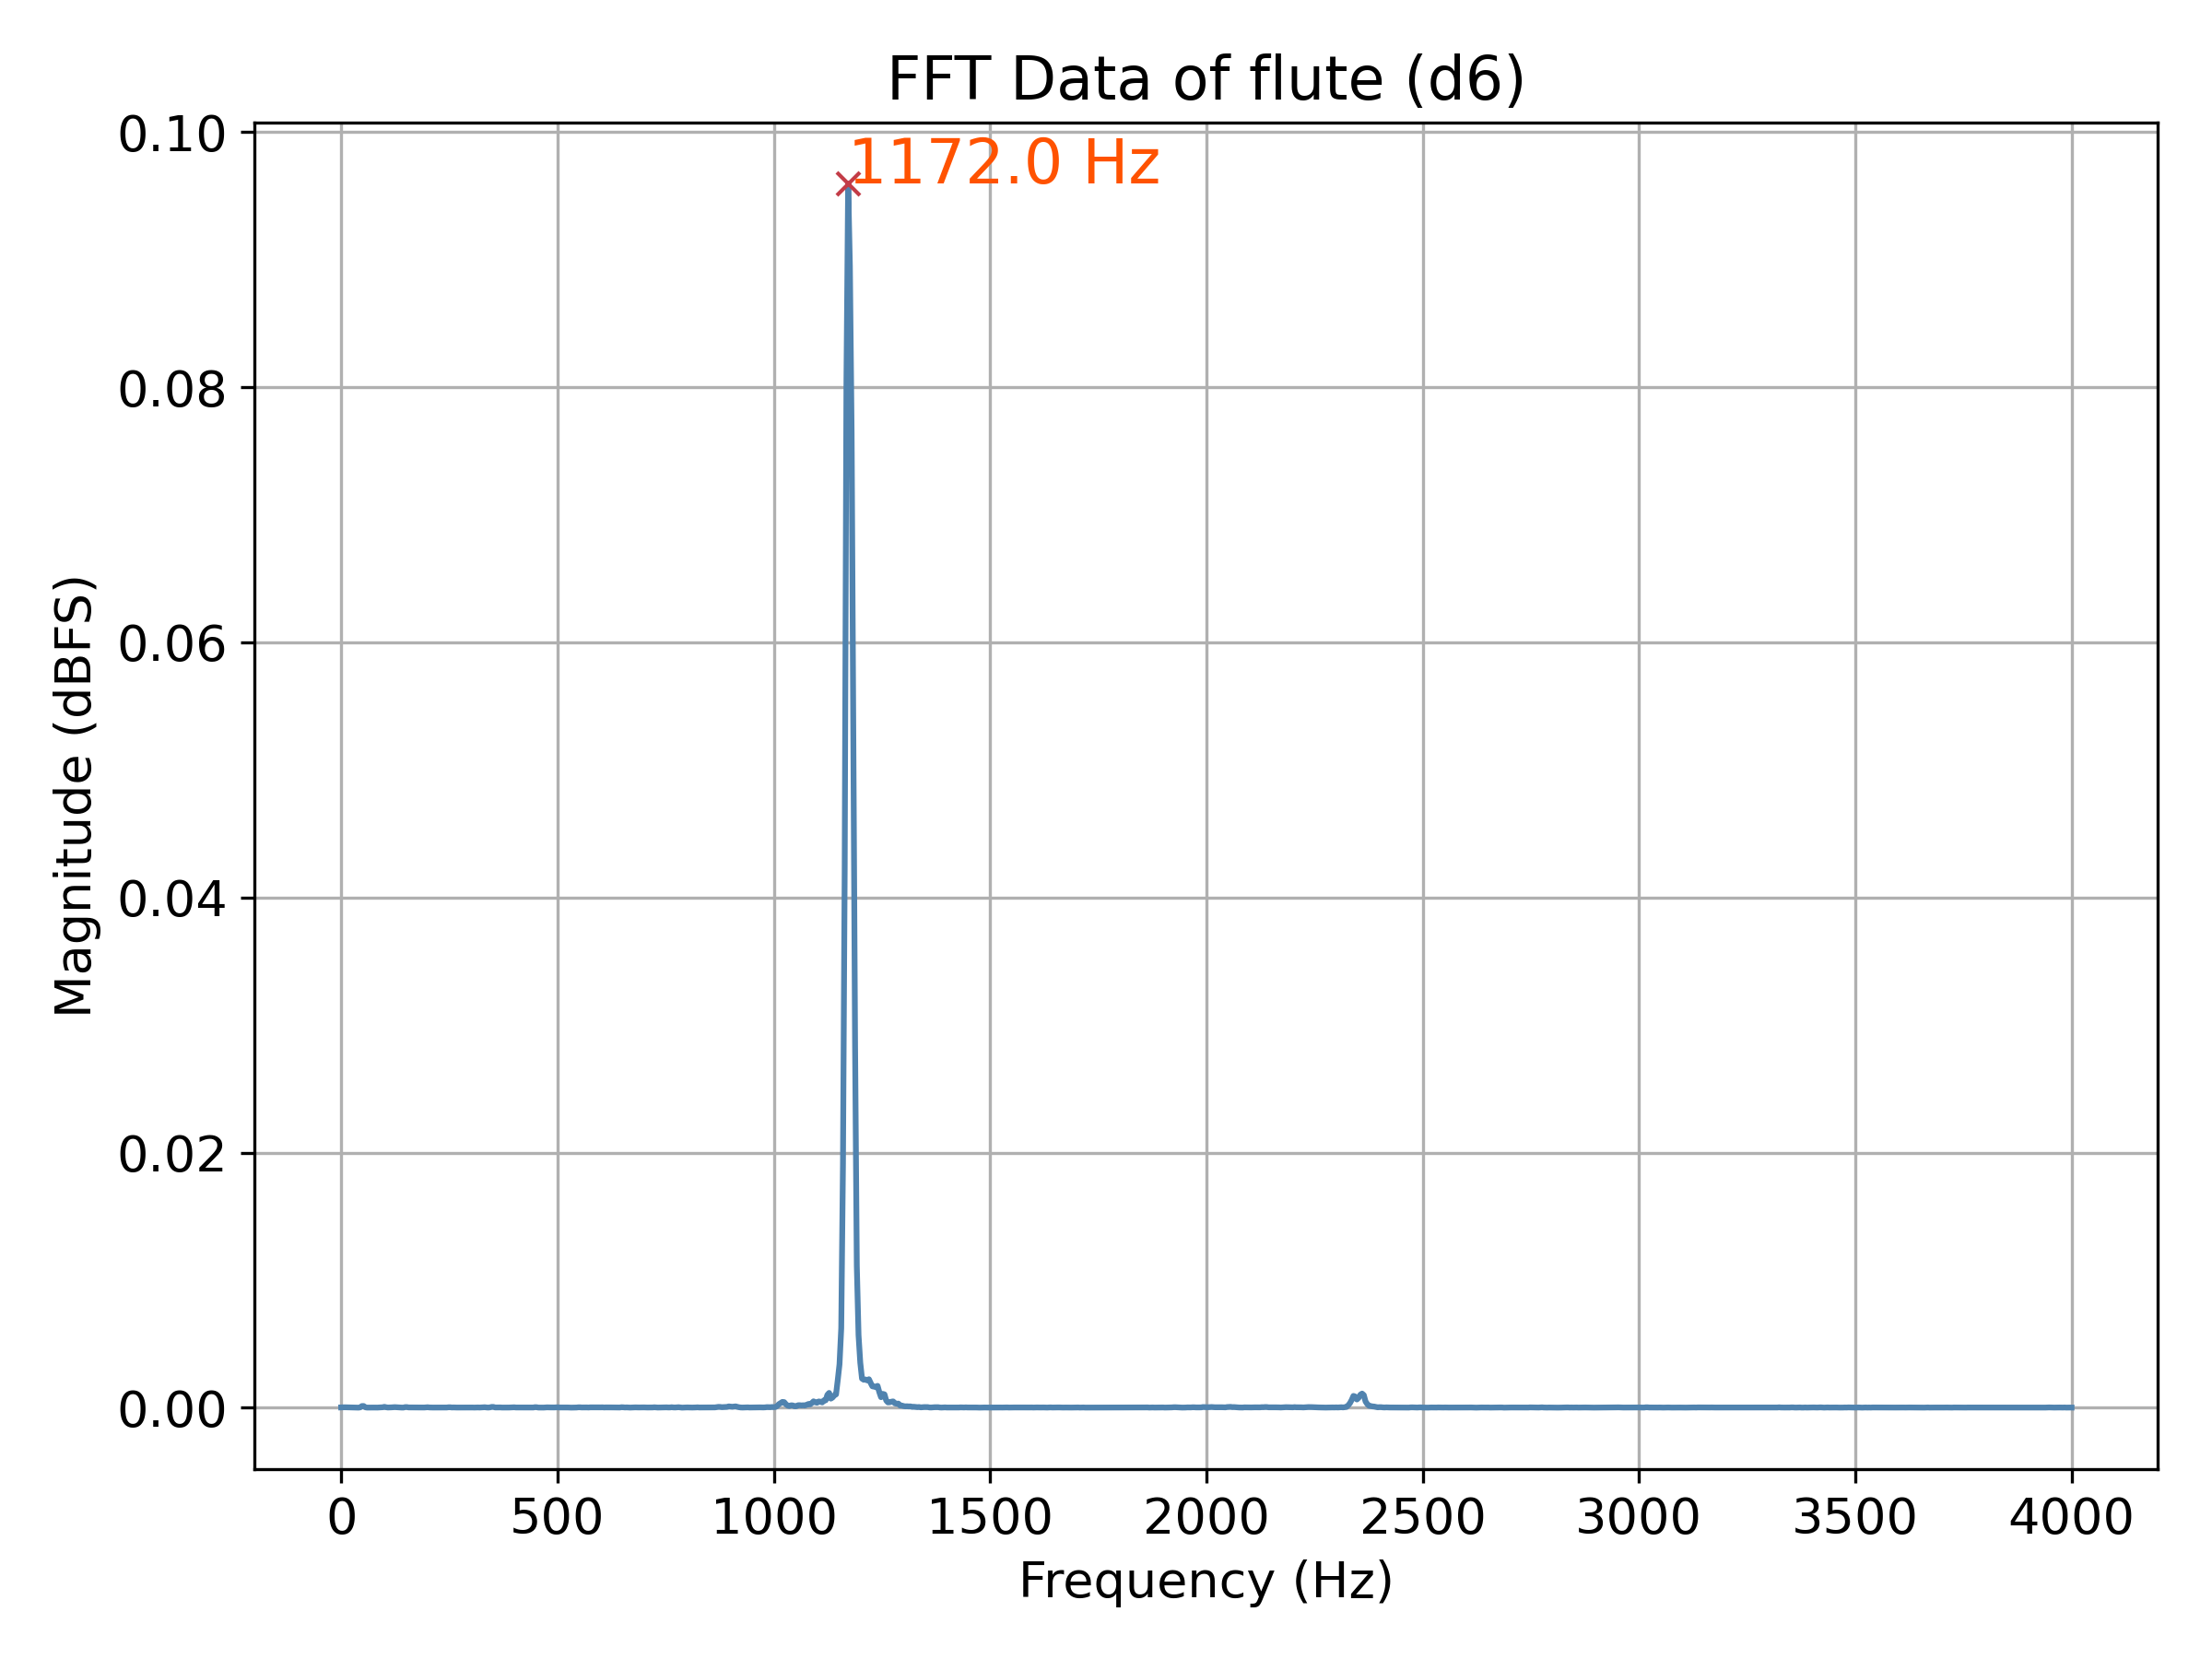
\includegraphics{/Users/kiloverse/Documents/物理学実験2/音のフーリエ解析/data/result_plot/4_fft_flute_d6.png}}}
          \caption{パンパイプD6音}
        \end{minipage}% % 在两个 minipage 环境之间使用 % 符号来消除之间的空白
        \begin{minipage}[b]{0.49\textwidth}
          \centering
          \fbox{\adjustbox{height=0.265\textheight,keepaspectratio}{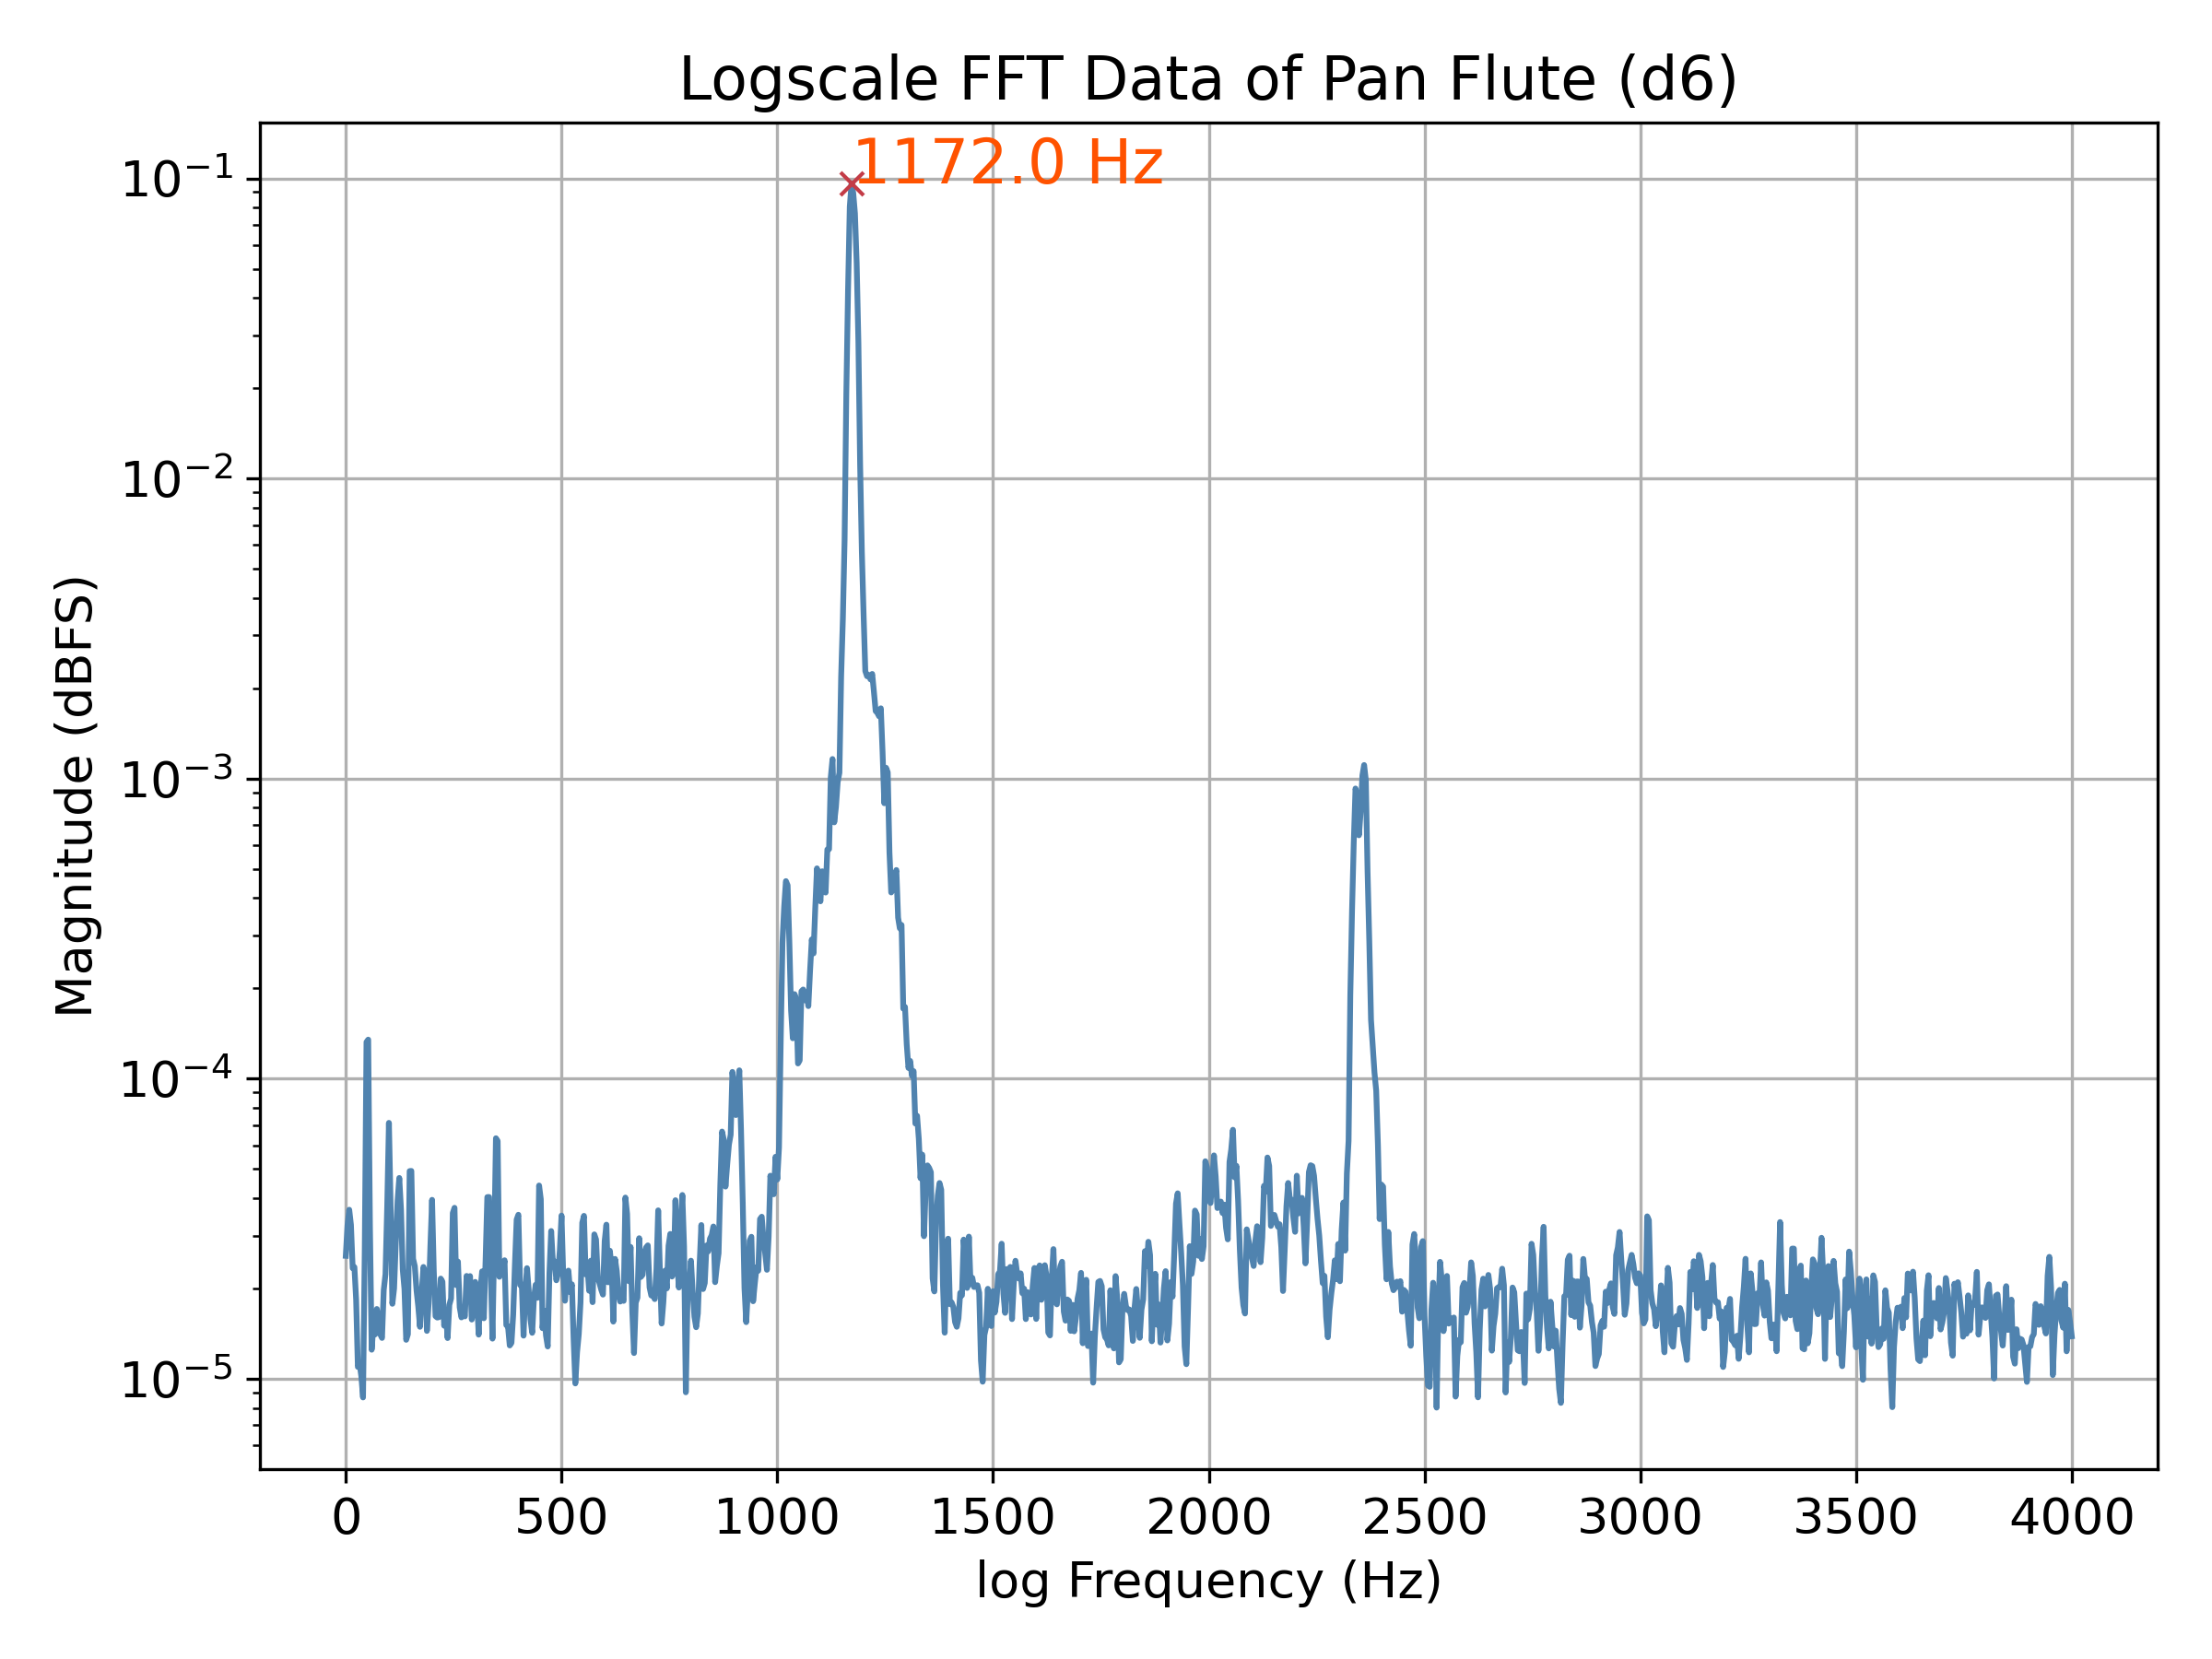
\includegraphics{/Users/kiloverse/Documents/物理学実験2/音のフーリエ解析/data/result_plot/4_fft_log_flute_d6.png}}}
          \caption{パンパイプD6音(y in logscale)}
        \end{minipage}
    \end{figure}
    \begin{figure}[htbp]
        \centering
        \begin{minipage}[b]{0.49\textwidth} % minipage 环境用于在同一行内并排放置内容,[b] 参数表示底部对齐,{0.5\textwidth} 设置 minipage 的宽度为页面宽度的一半
          \centering
          \fbox{\adjustbox{height=0.265\textheight,keepaspectratio}{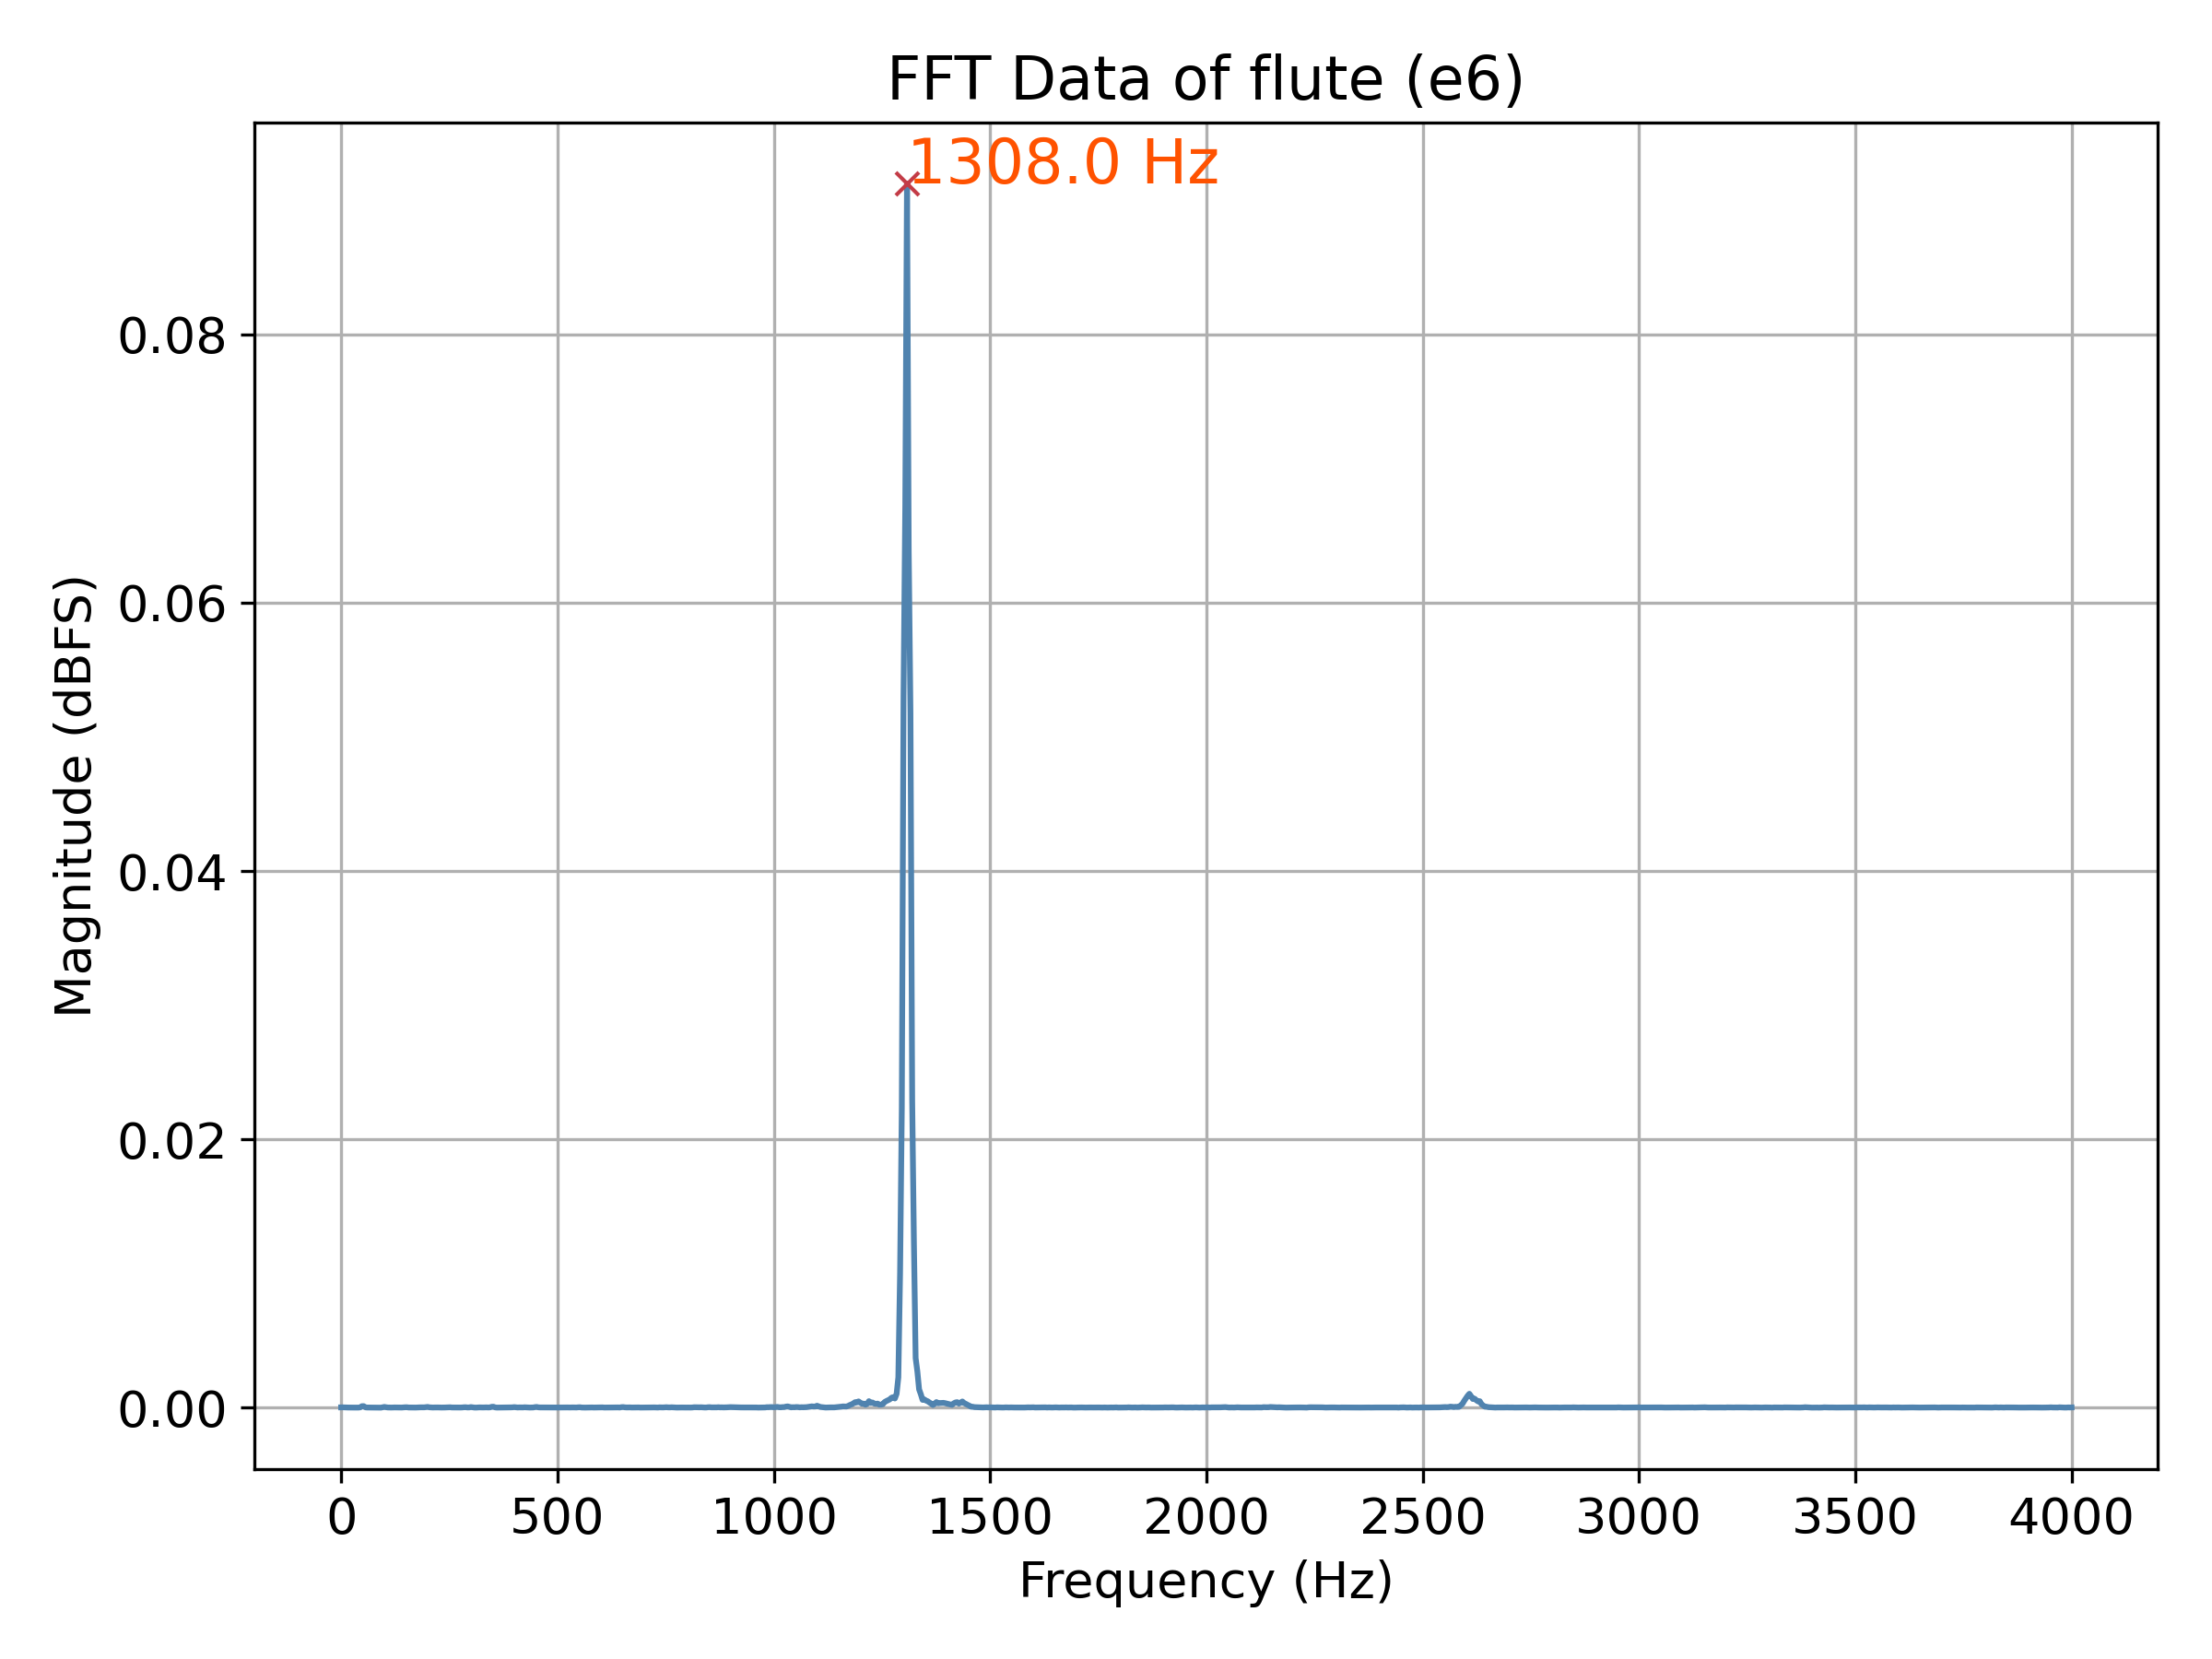
\includegraphics{/Users/kiloverse/Documents/物理学実験2/音のフーリエ解析/data/result_plot/4_fft_flute_e6.png}}}
          \caption{パンパイプE6音}
        \end{minipage}% % 在两个 minipage 环境之间使用 % 符号来消除之间的空白
        \begin{minipage}[b]{0.49\textwidth}
          \centering
          \fbox{\adjustbox{height=0.265\textheight,keepaspectratio}{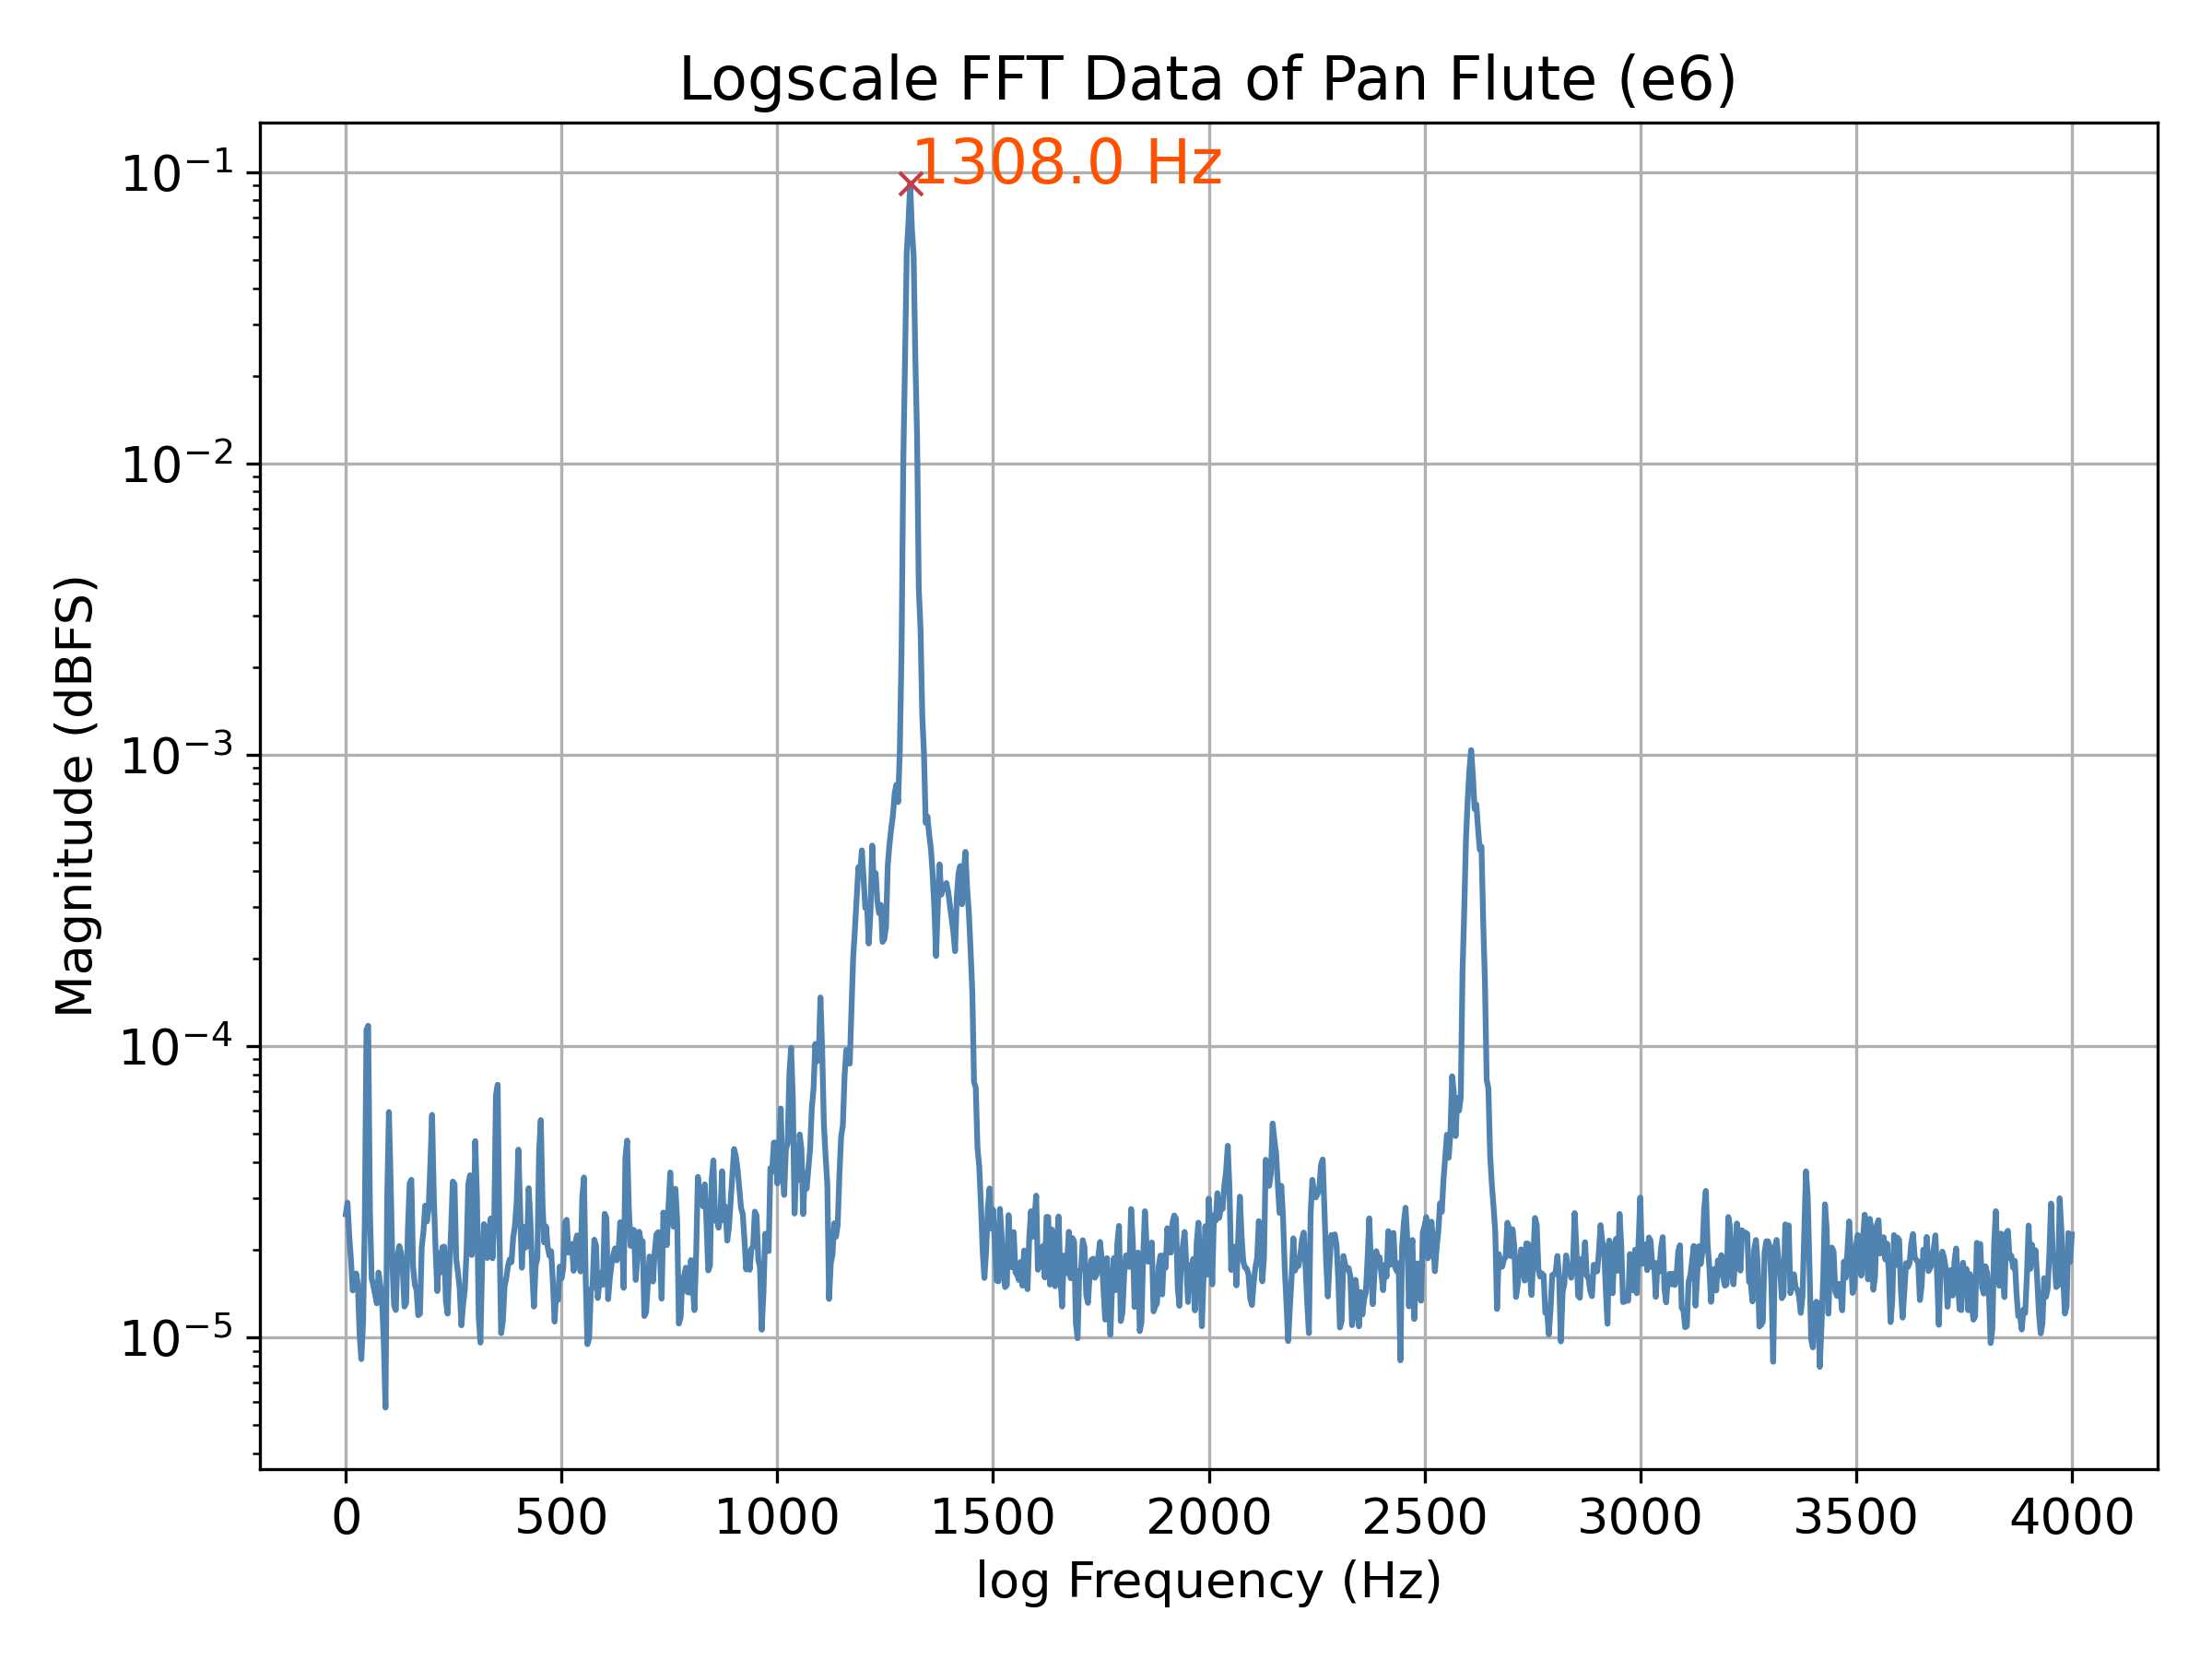
\includegraphics{/Users/kiloverse/Documents/物理学実験2/音のフーリエ解析/data/result_plot/4_fft_log_flute_e6.png}}}
          \caption{パンパイプE6音(y in logscale)}
        \end{minipage}
    \end{figure}
    \FloatBarrier

    次に、金管楽器であるトランペットの$B^{b}$4、C5、E5の周波数成分を分析した。
    \begin{figure}[htbp]
        \centering
        \begin{minipage}[b]{0.49\textwidth} % minipage 环境用于在同一行内并排放置内容,[b] 参数表示底部对齐,{0.5\textwidth} 设置 minipage 的宽度为页面宽度的一半
          \centering
          \fbox{\adjustbox{height=0.265\textheight,keepaspectratio}{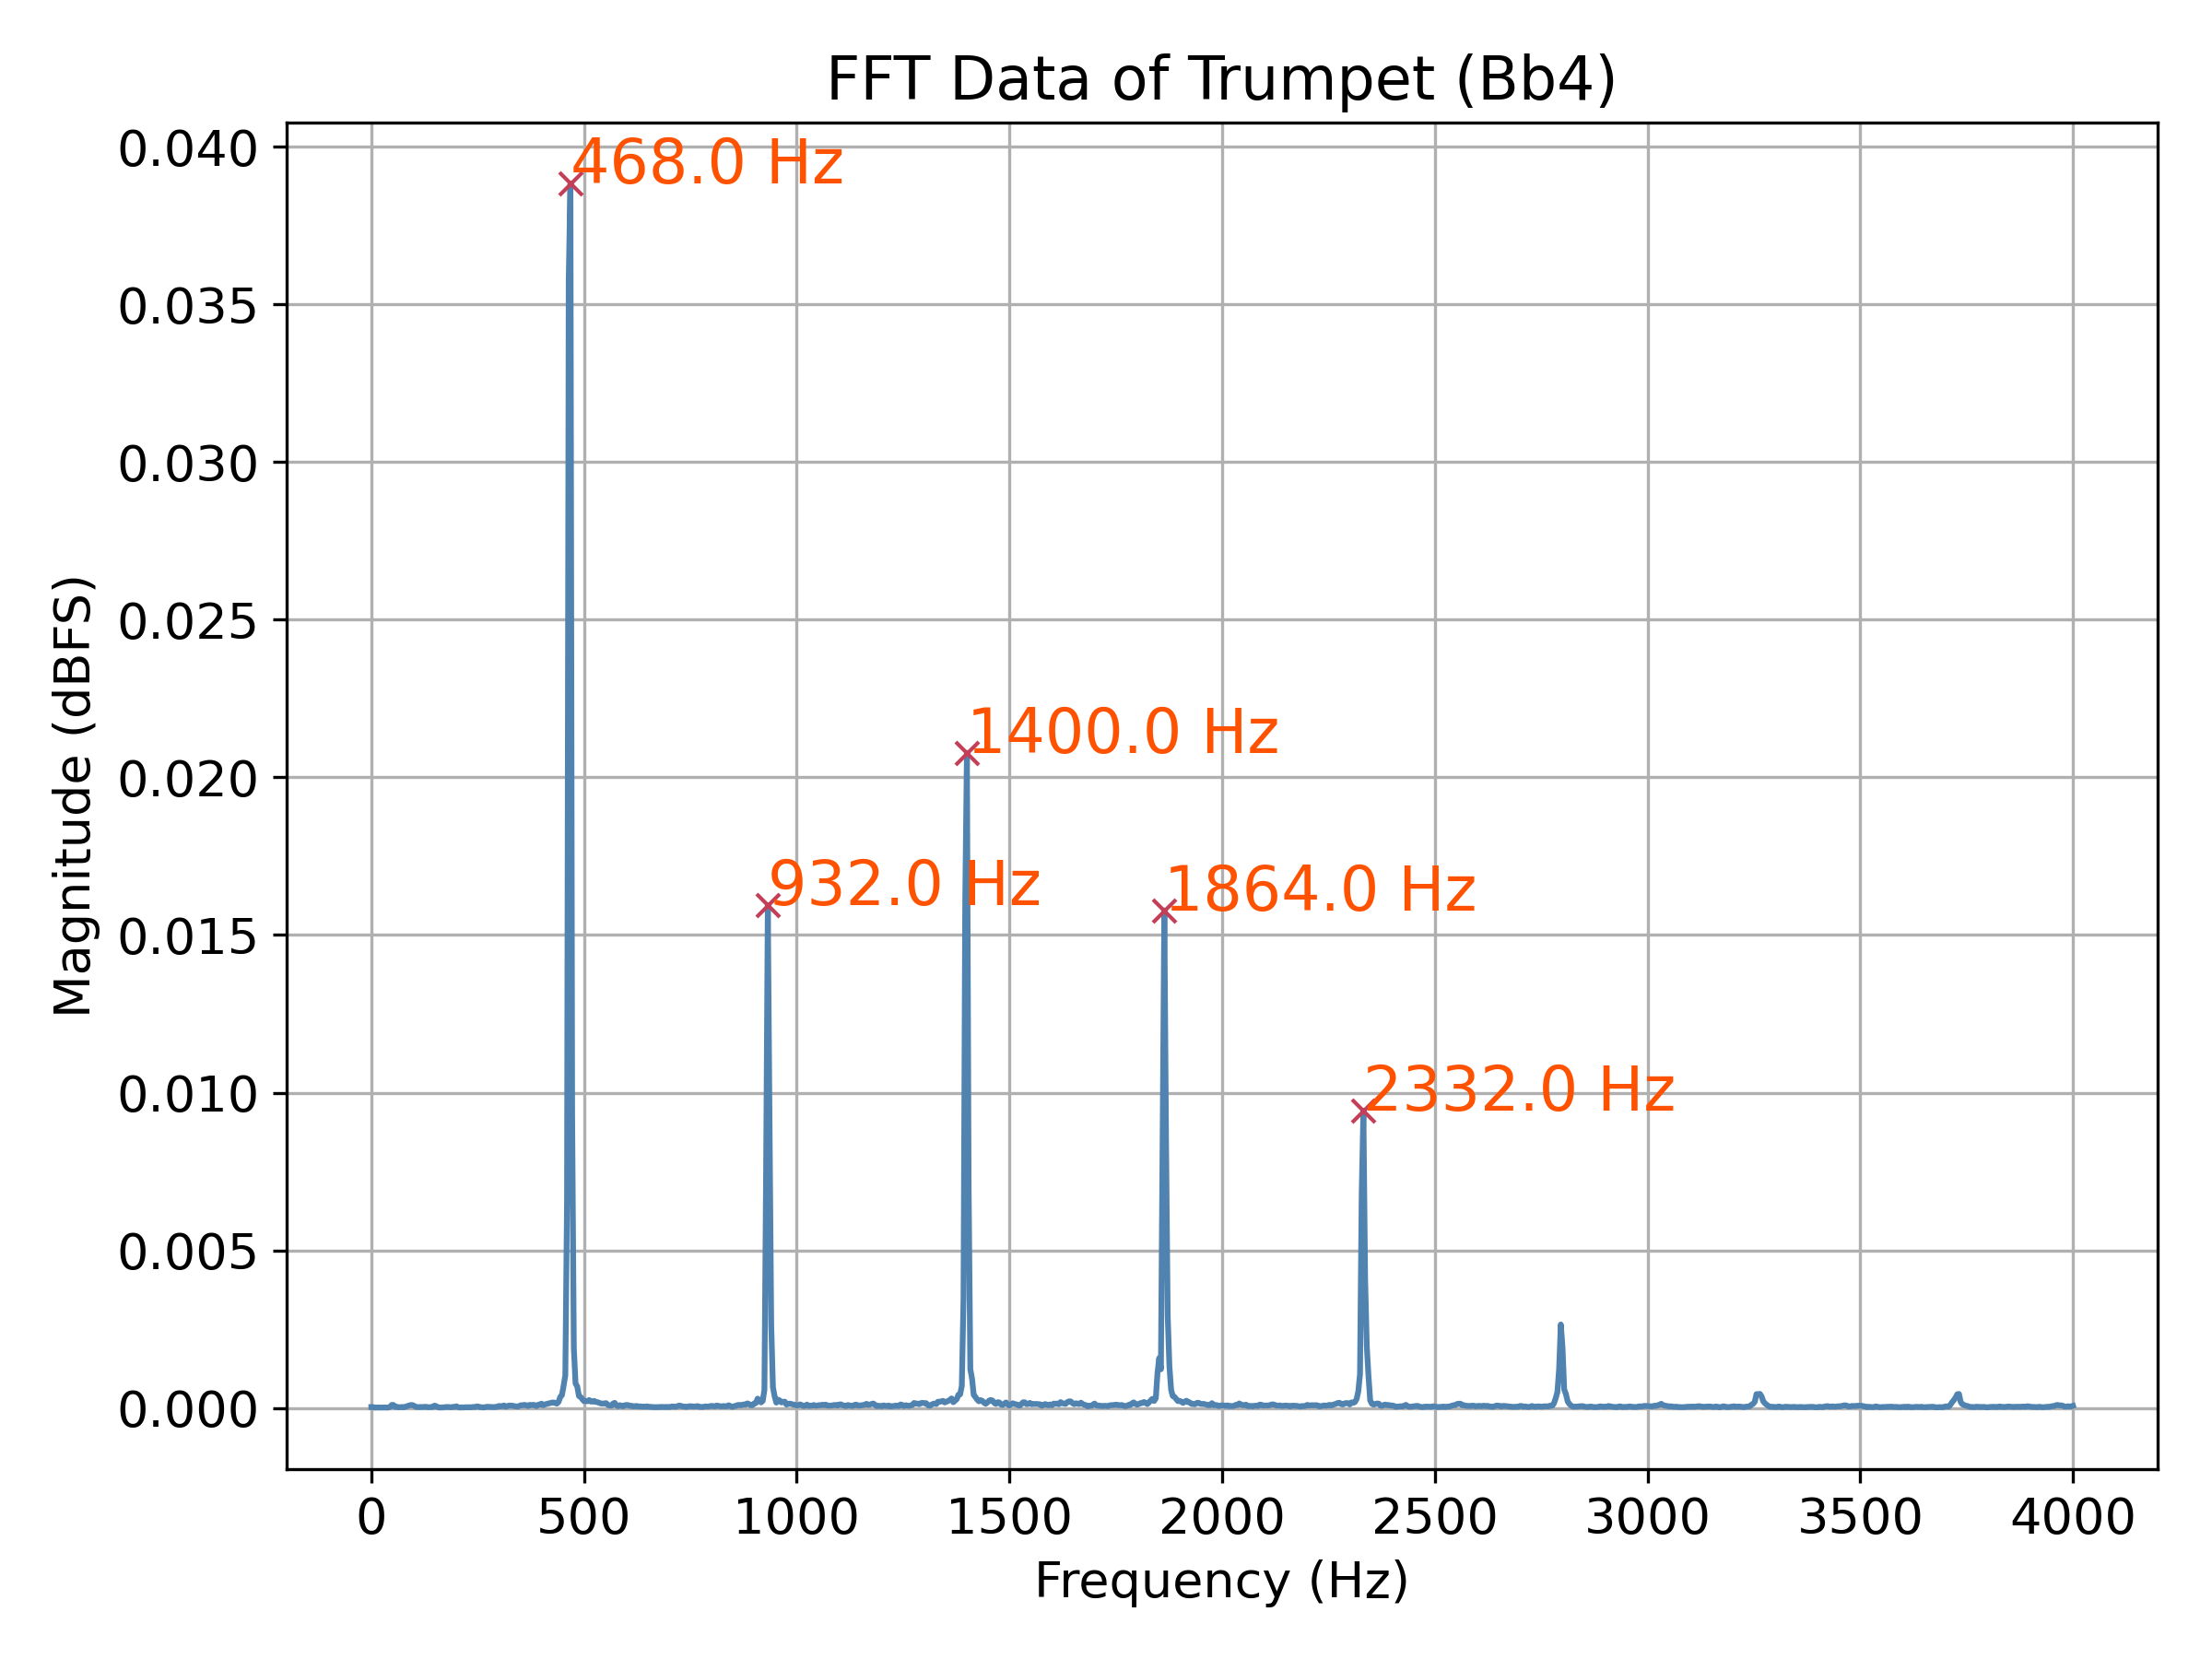
\includegraphics{/Users/kiloverse/Documents/物理学実験2/音のフーリエ解析/data/result_plot/4_fft_tram_Bb4.png}}}
          \caption{トランペット$B^{b}$4音}
        \end{minipage}% % 在两个 minipage 环境之间使用 % 符号来消除之间的空白
        \begin{minipage}[b]{0.49\textwidth}
          \centering
          \fbox{\adjustbox{height=0.265\textheight,keepaspectratio}{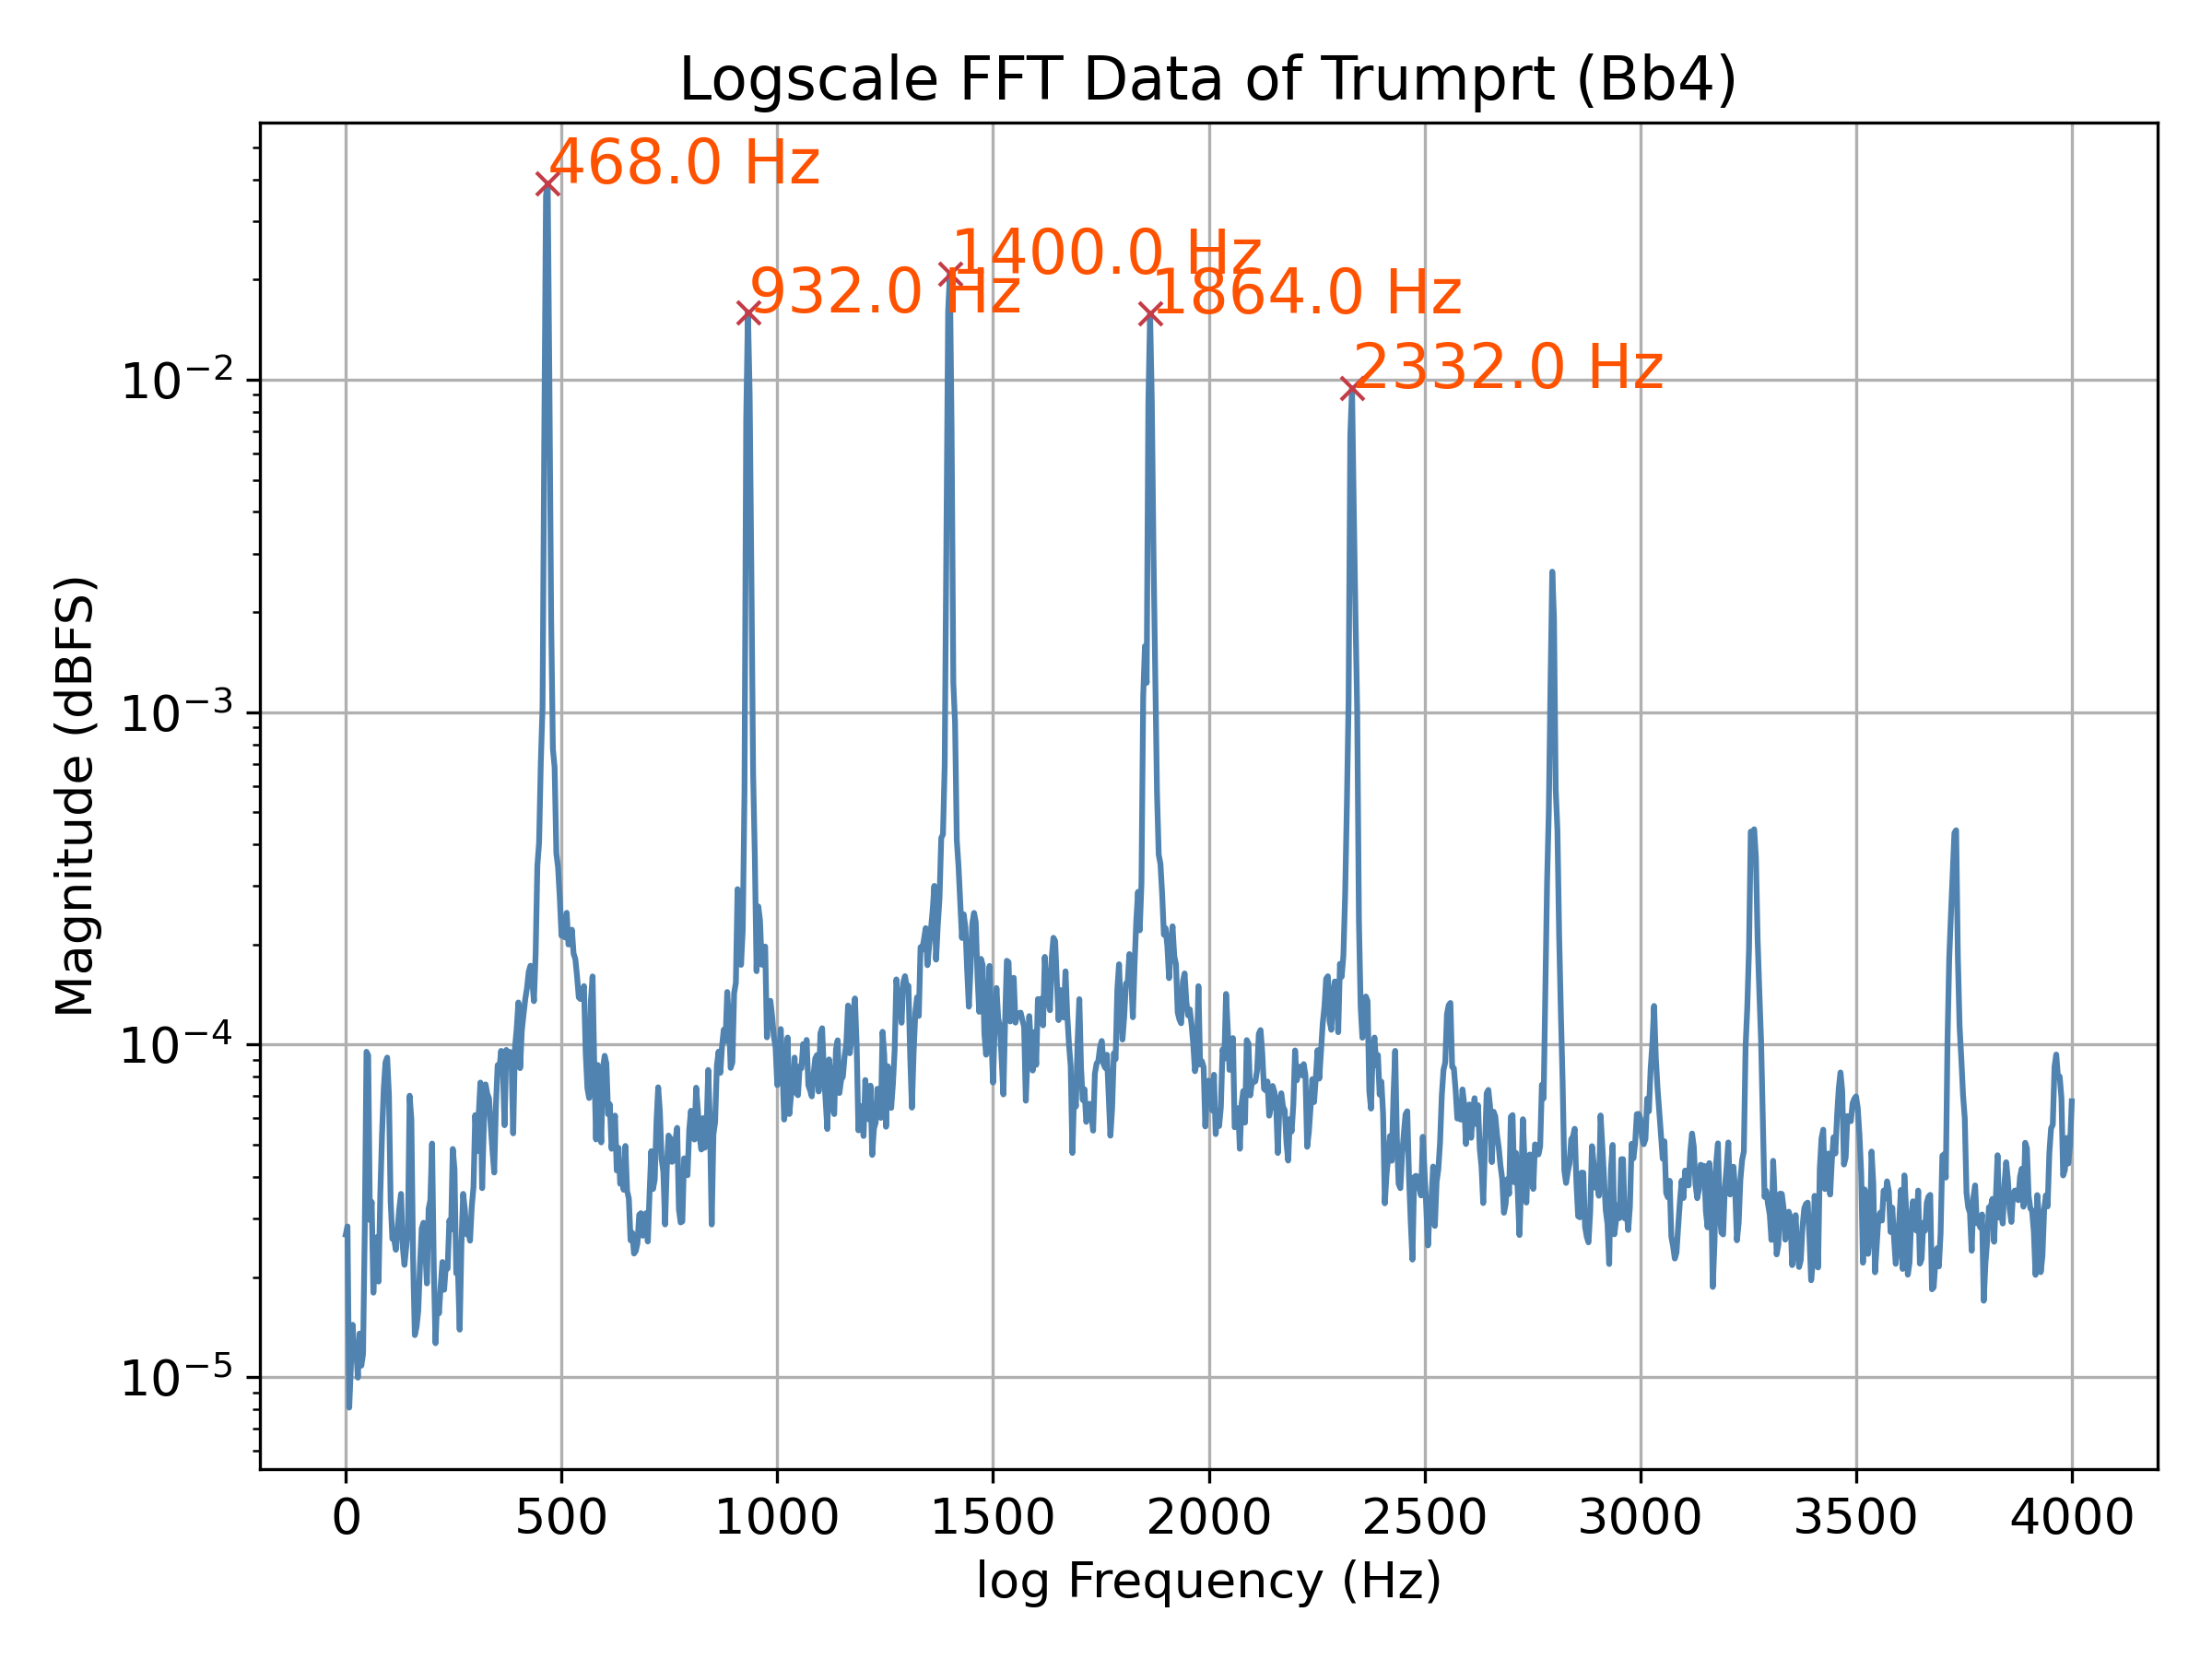
\includegraphics{/Users/kiloverse/Documents/物理学実験2/音のフーリエ解析/data/result_plot/4_fft_log_tram_Bb4.png}}}
          \caption{トランペット$B^{b}$4音(y in logscale)}
        \end{minipage}
    \end{figure}
    \begin{figure}[htbp]
        \centering
        \begin{minipage}[b]{0.49\textwidth} % minipage 环境用于在同一行内并排放置内容,[b] 参数表示底部对齐,{0.5\textwidth} 设置 minipage 的宽度为页面宽度的一半
          \centering
          \fbox{\adjustbox{height=0.265\textheight,keepaspectratio}{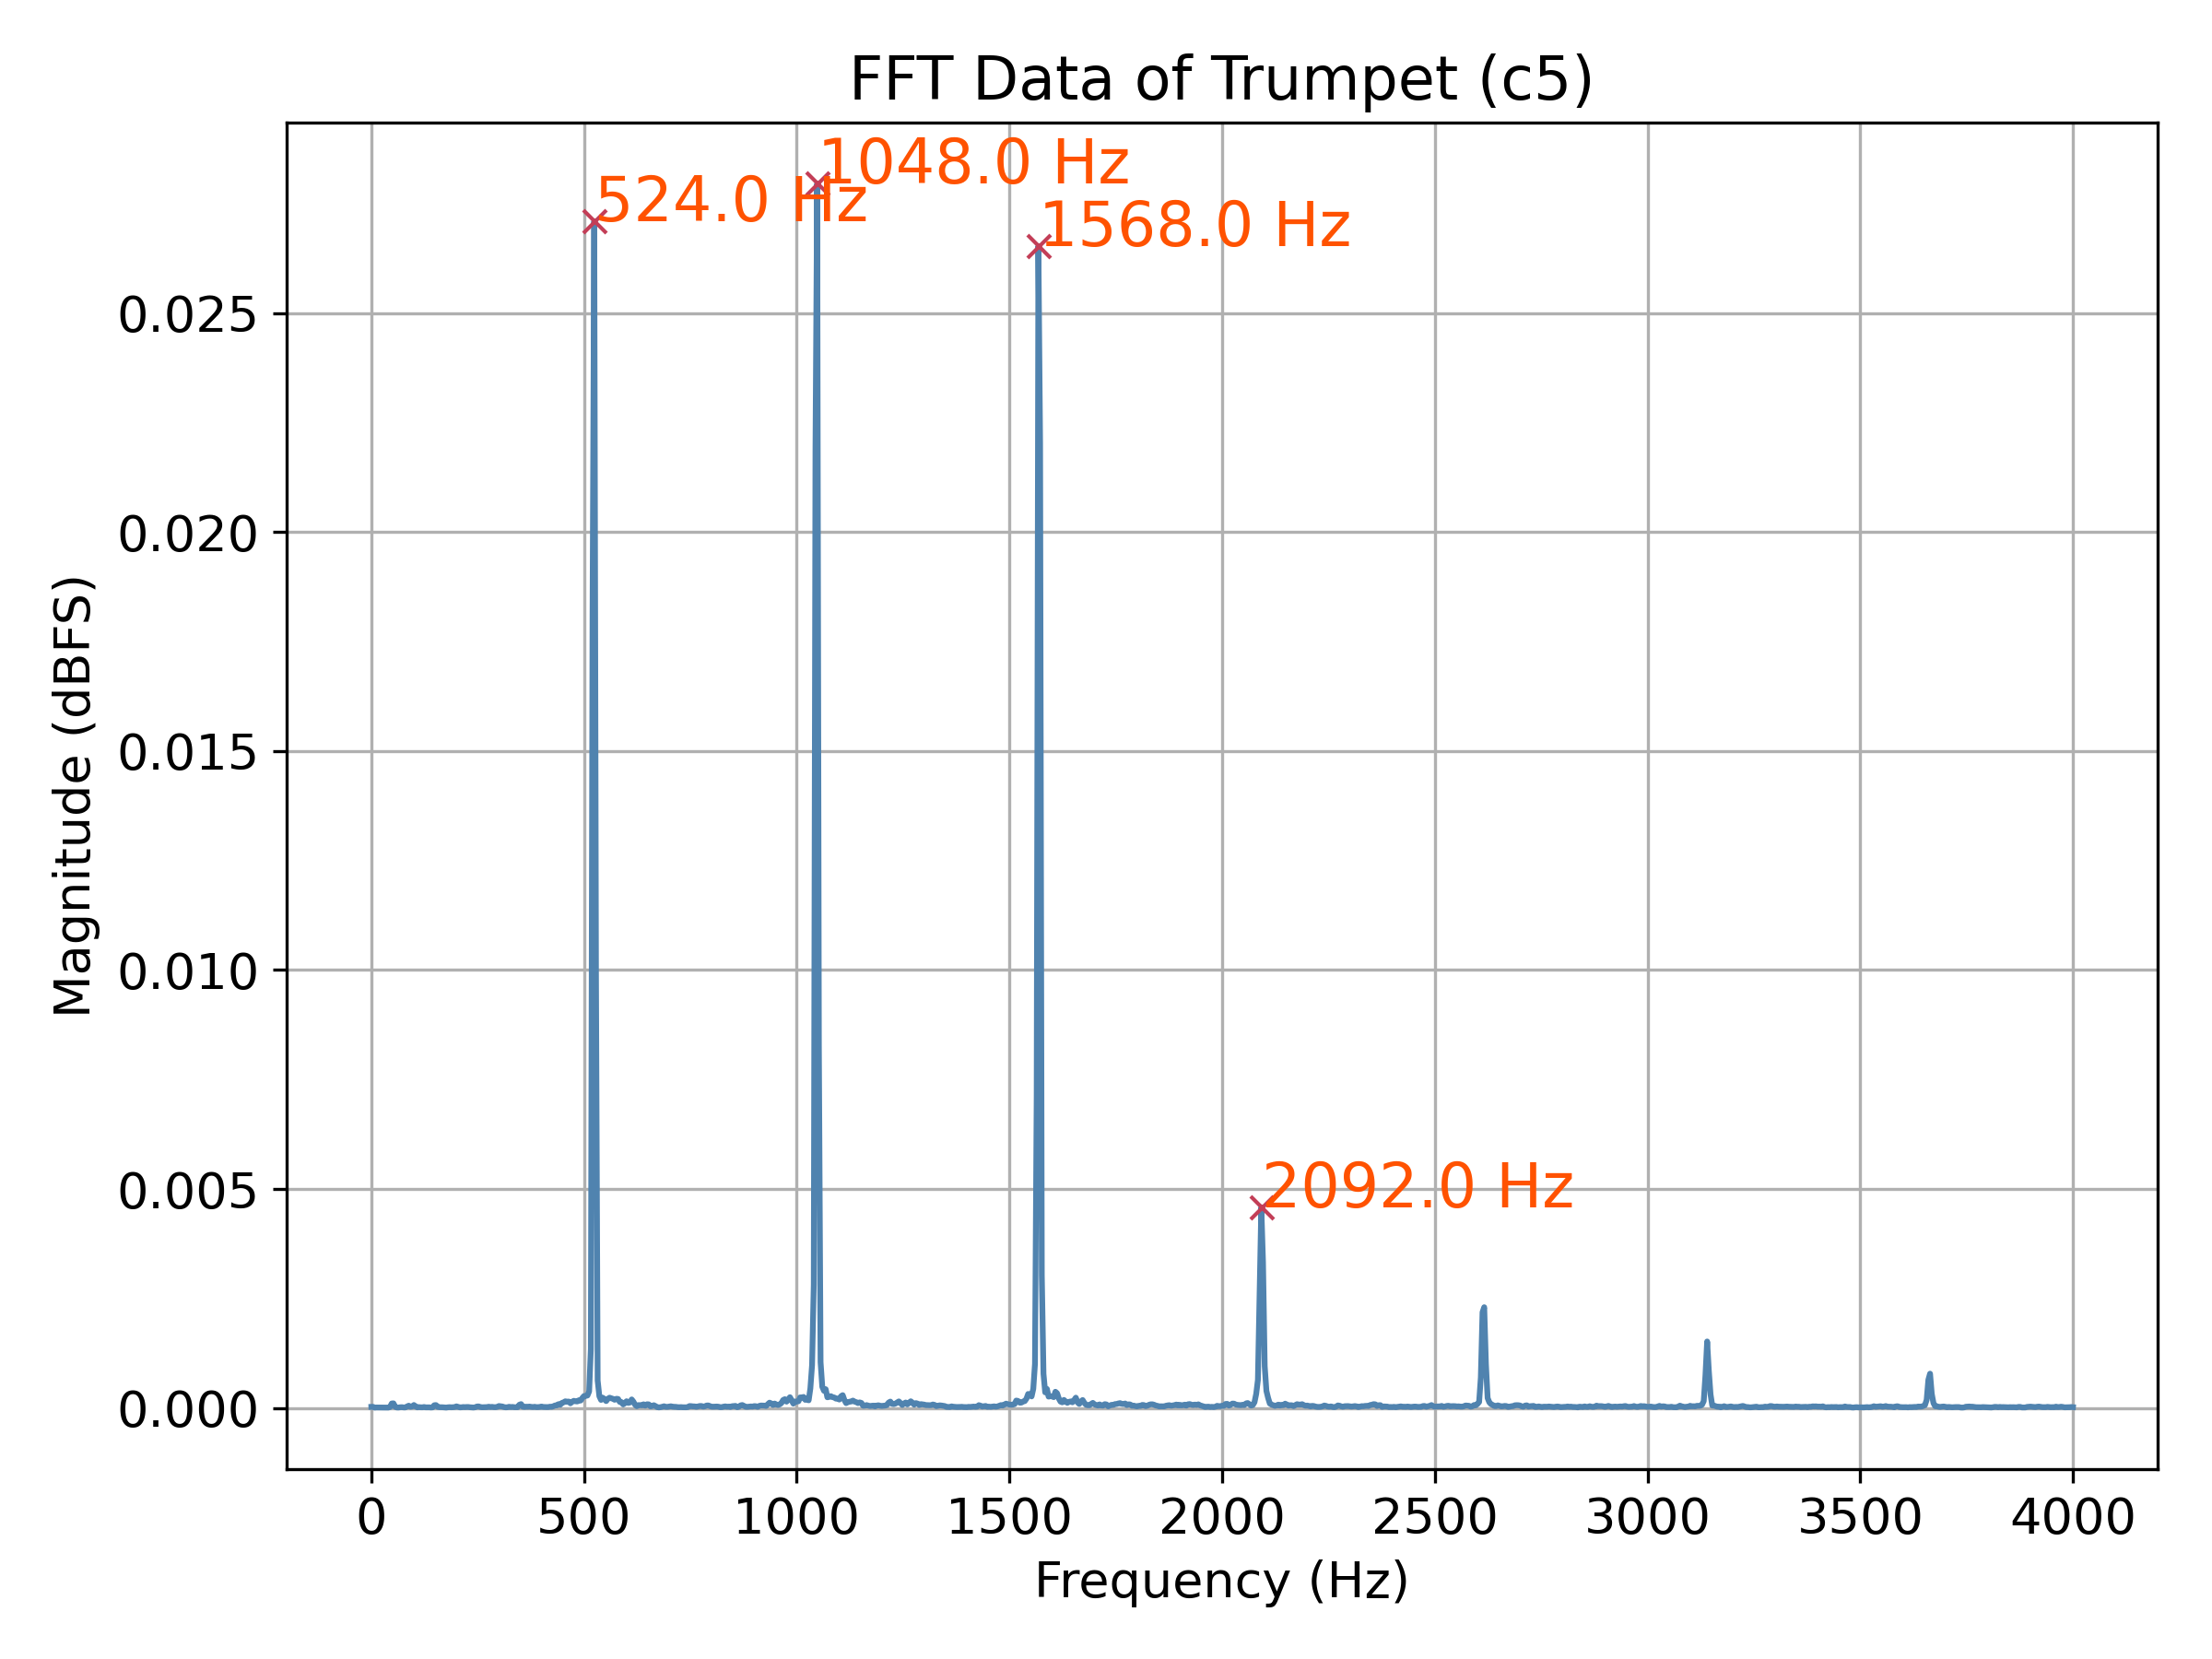
\includegraphics{/Users/kiloverse/Documents/物理学実験2/音のフーリエ解析/data/result_plot/4_fft_tram_c5.png}}}
          \caption{トランペットC5音}
        \end{minipage}% % 在两个 minipage 环境之间使用 % 符号来消除之间的空白
        \begin{minipage}[b]{0.49\textwidth}
          \centering
          \fbox{\adjustbox{height=0.265\textheight,keepaspectratio}{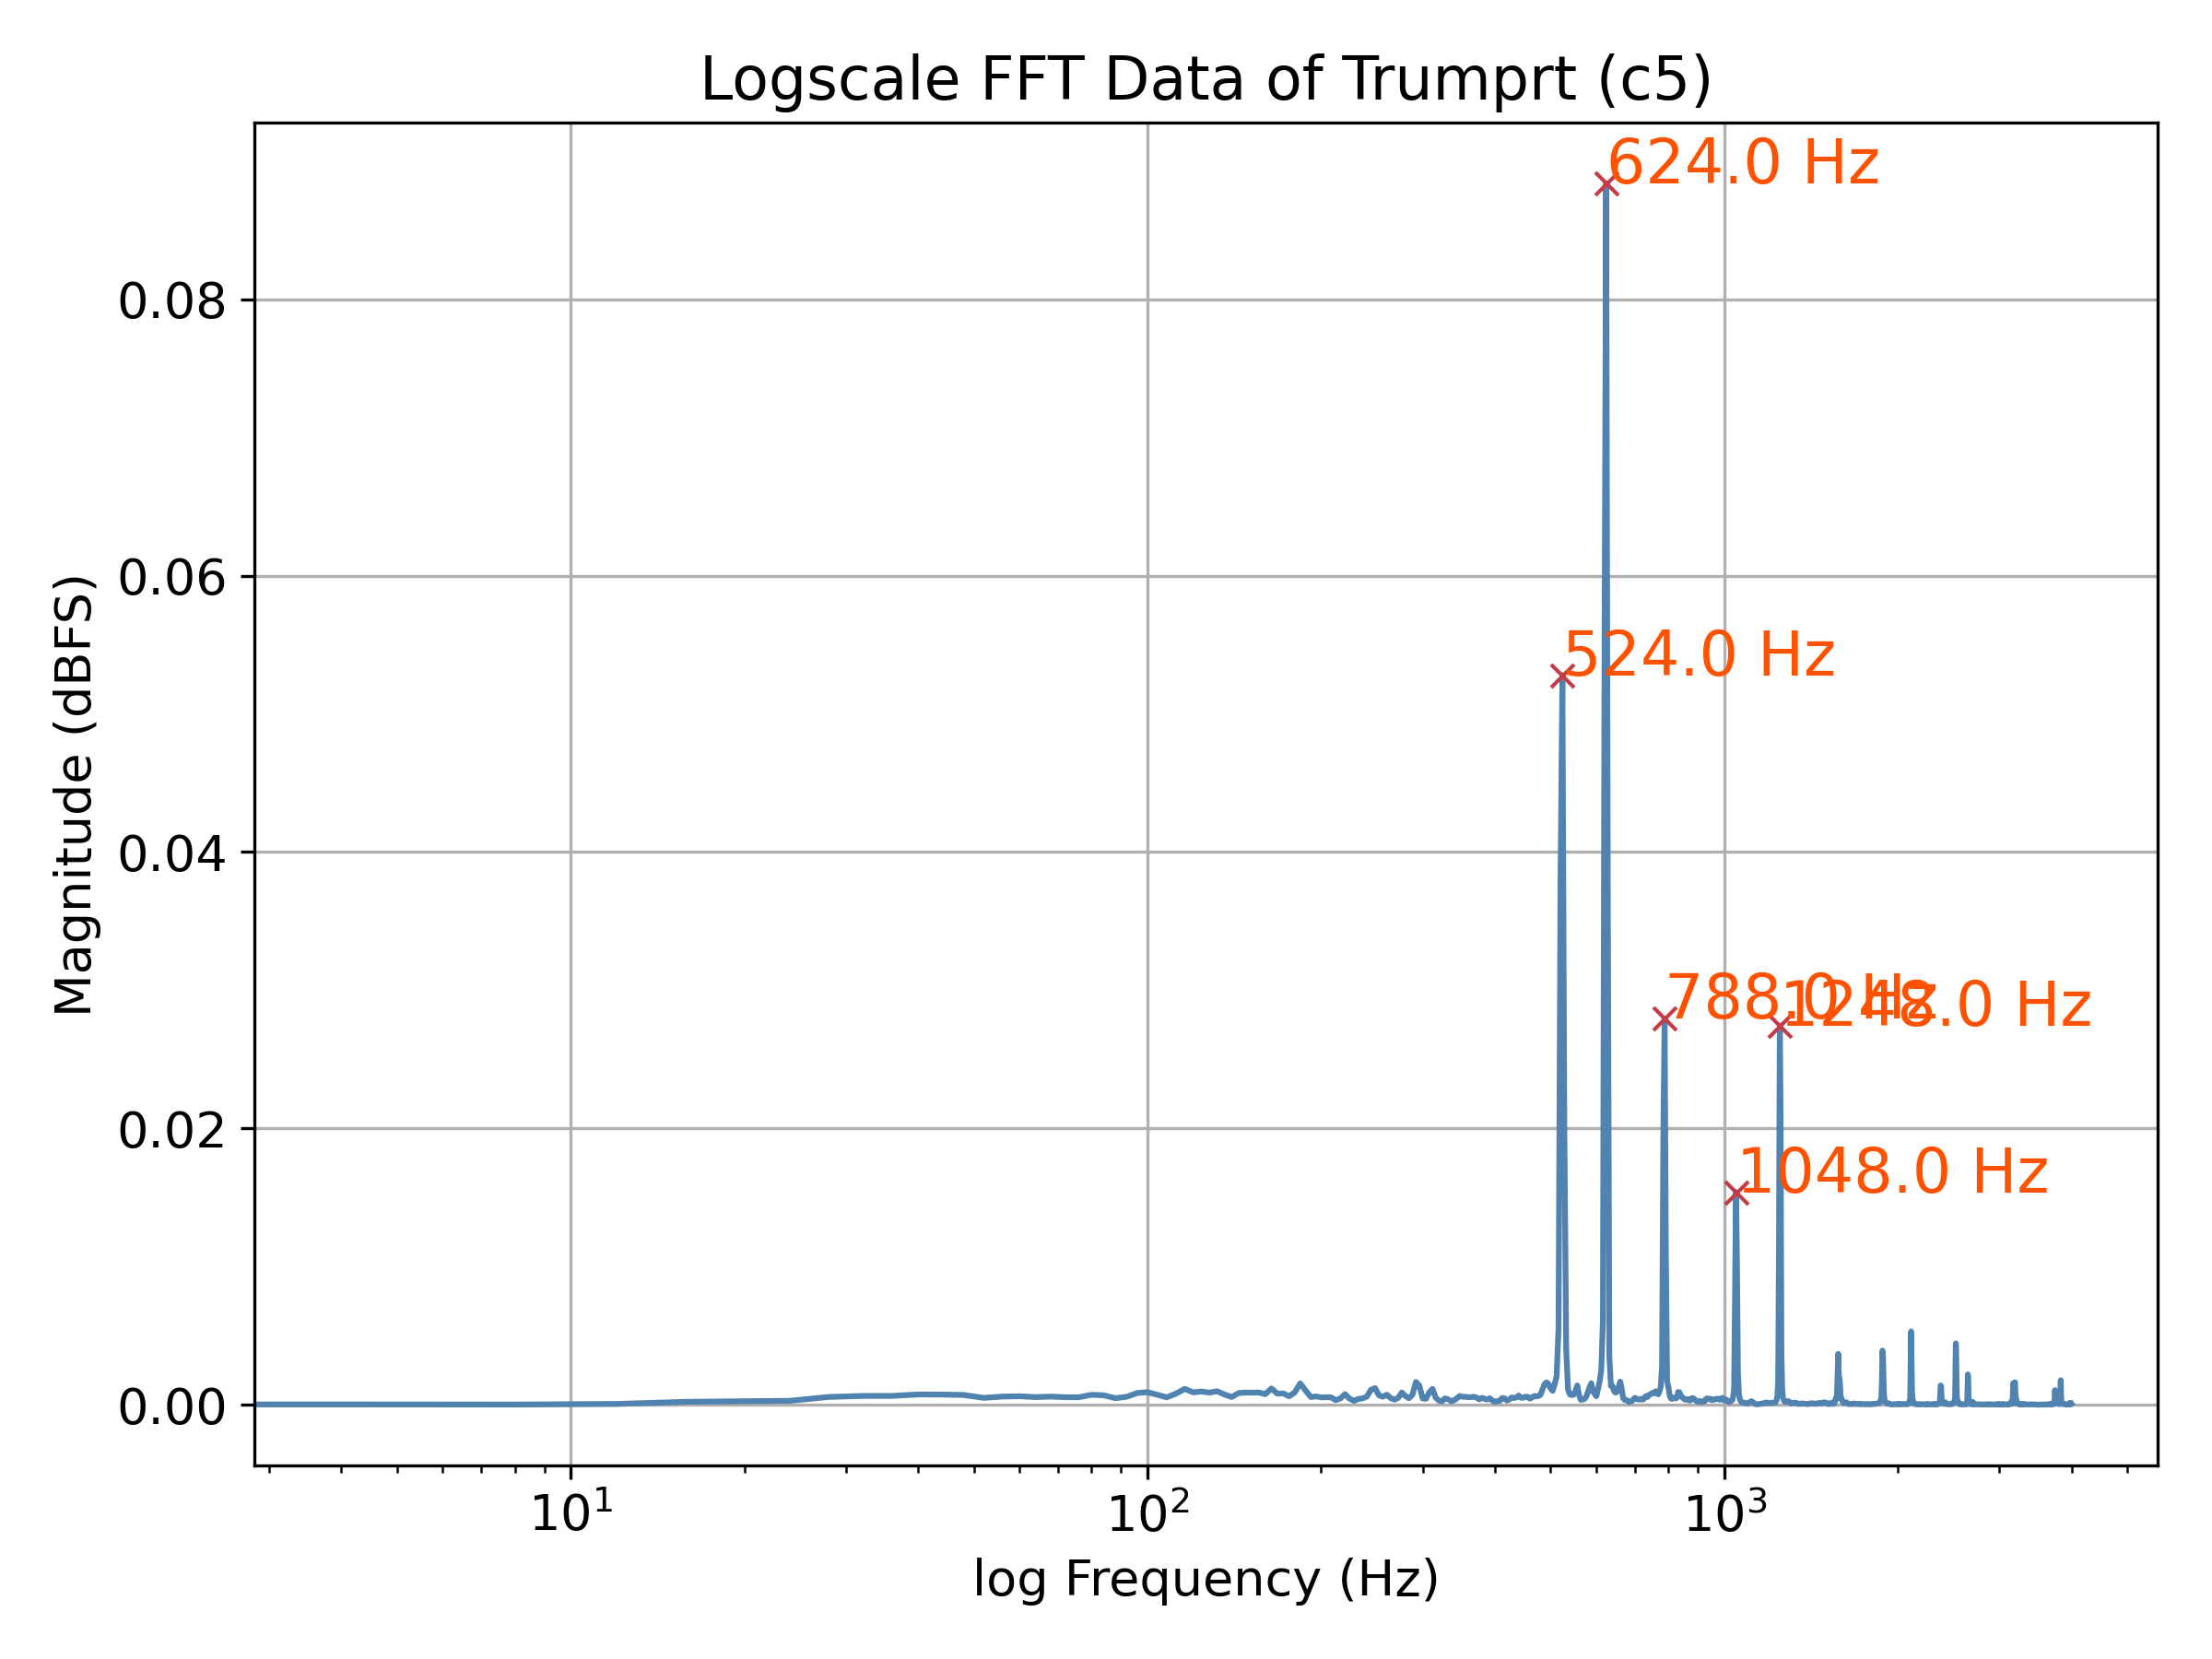
\includegraphics{/Users/kiloverse/Documents/物理学実験2/音のフーリエ解析/data/result_plot/4_fft_log_tram_c5.png}}}
          \caption{トランペットC5音(y in logscale)}
        \end{minipage}
    \end{figure}
    \begin{figure}[htbp]
        \centering
        \begin{minipage}[b]{0.49\textwidth} % minipage 环境用于在同一行内并排放置内容,[b] 参数表示底部对齐,{0.5\textwidth} 设置 minipage 的宽度为页面宽度的一半
          \centering
          \fbox{\adjustbox{height=0.265\textheight,keepaspectratio}{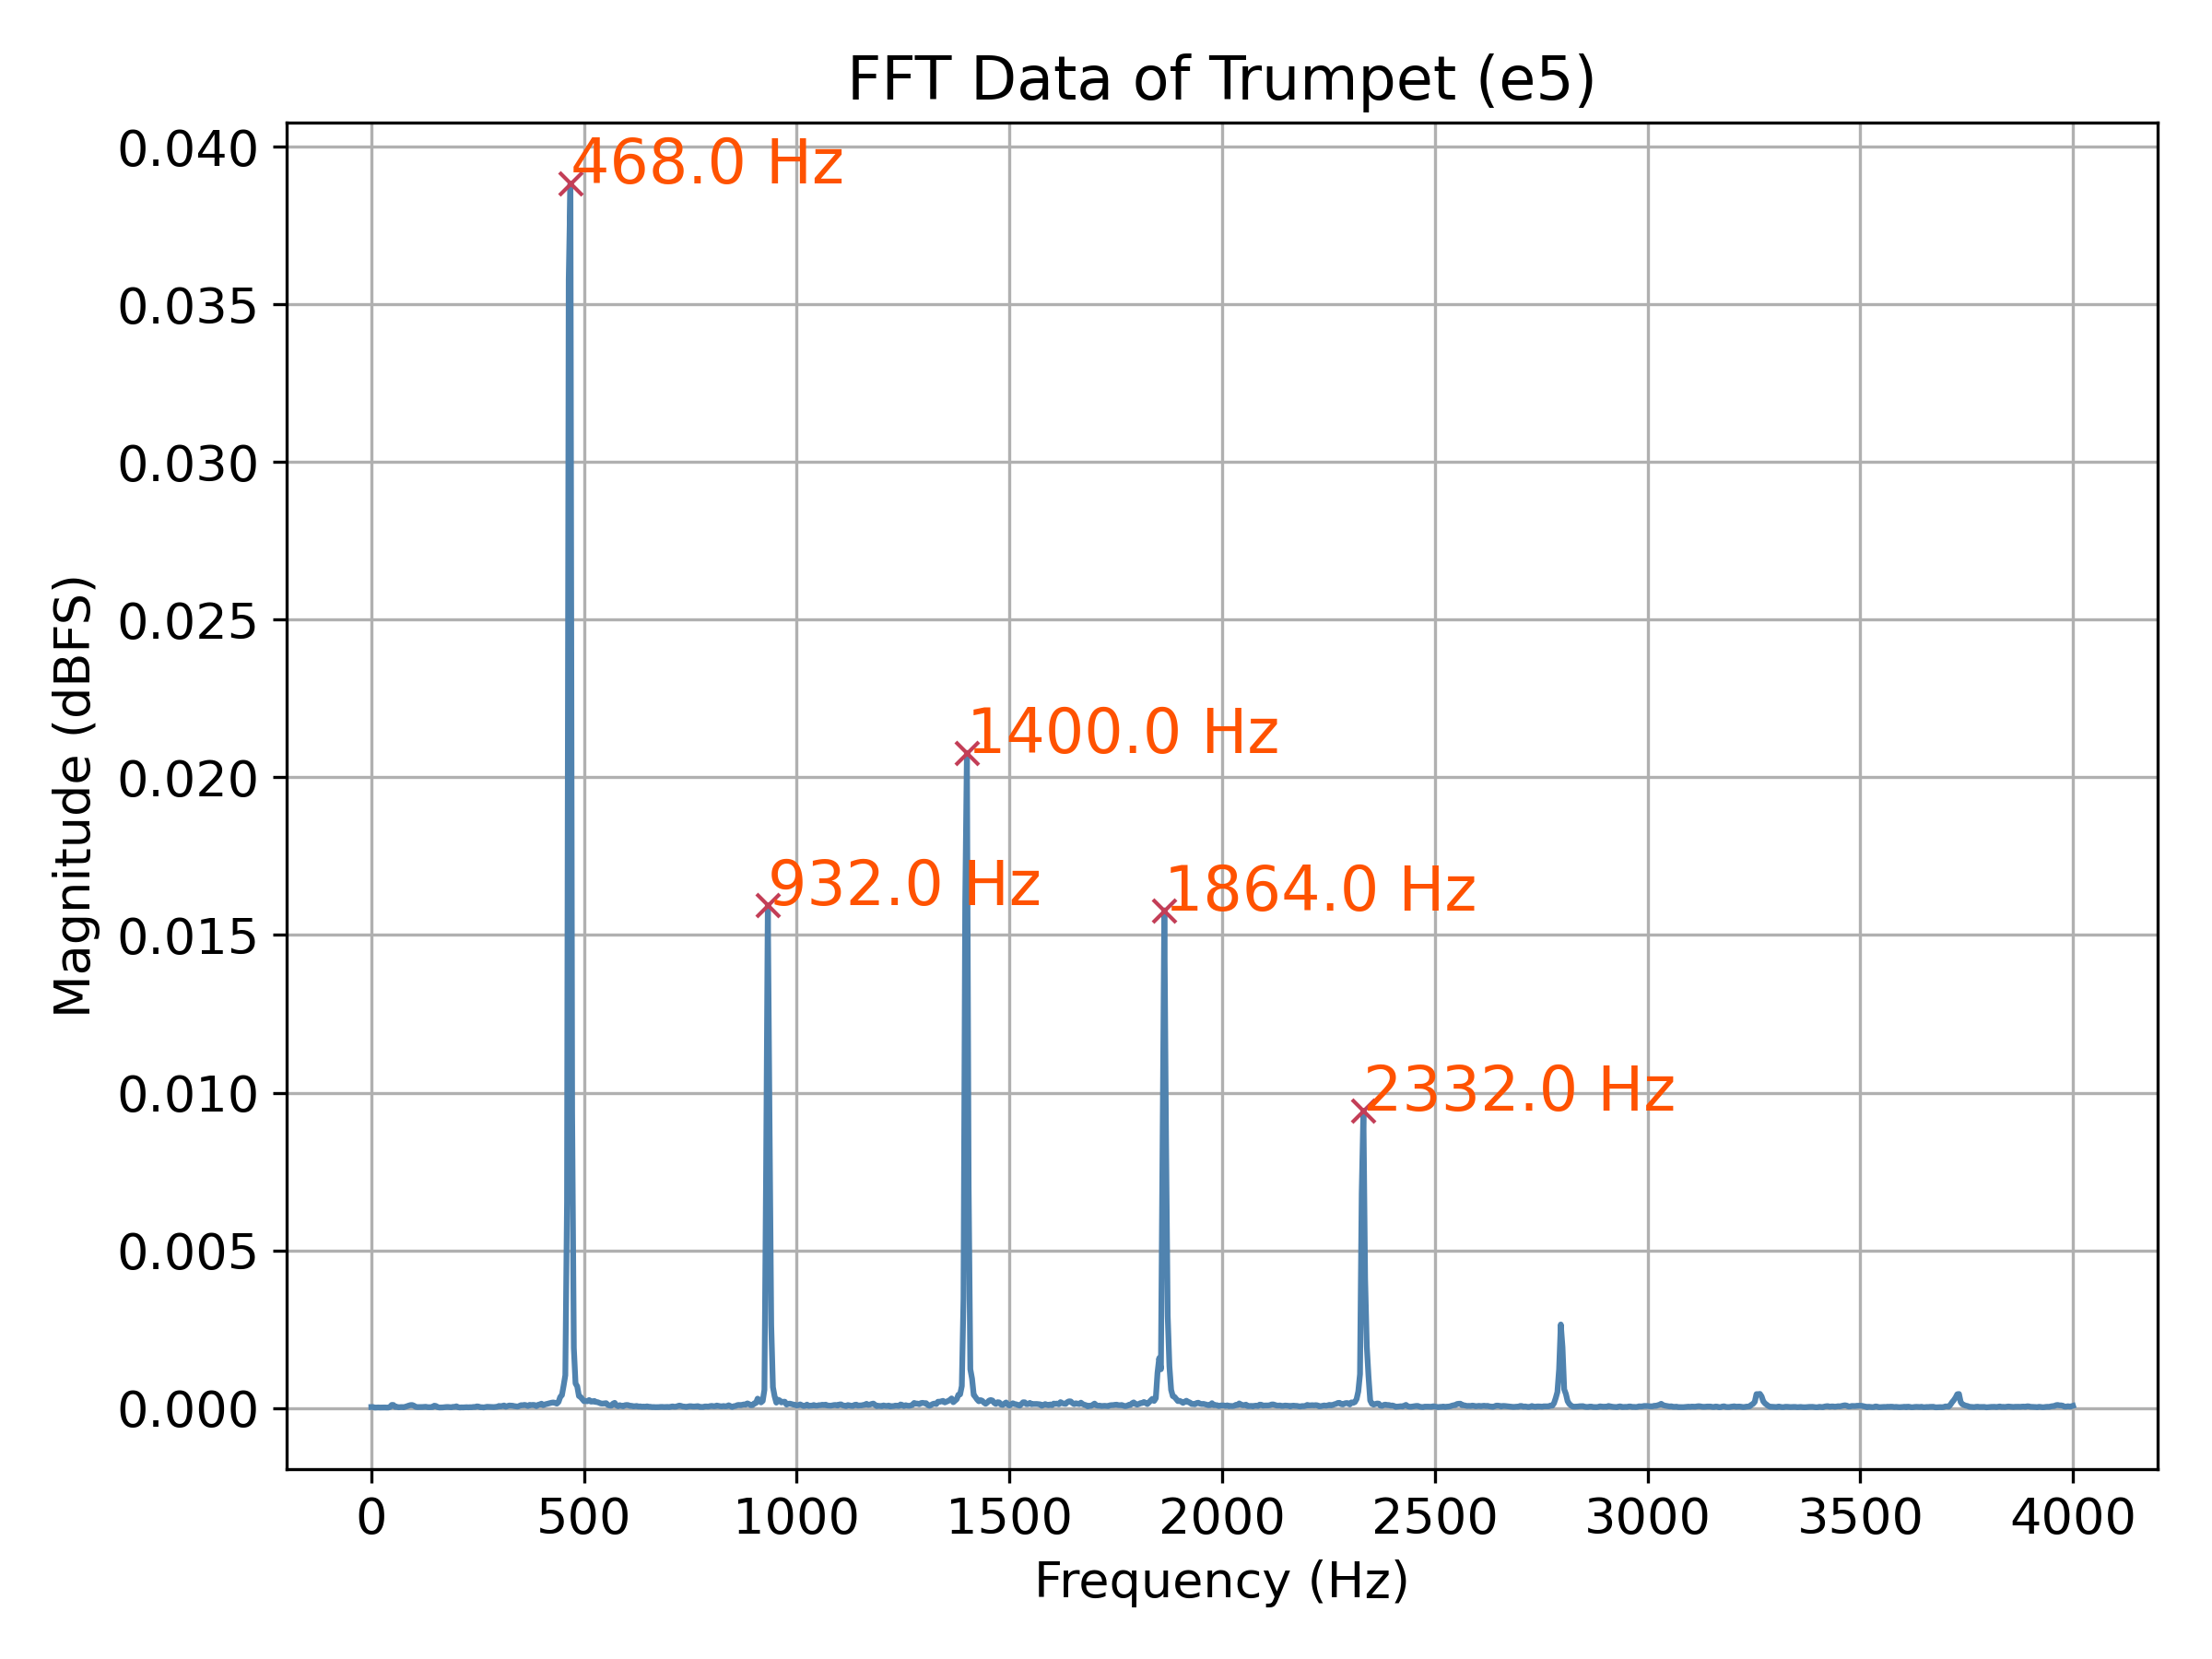
\includegraphics{/Users/kiloverse/Documents/物理学実験2/音のフーリエ解析/data/result_plot/4_fft_tram_e5.png}}}
          \caption{パンパイプE5音}
        \end{minipage}% % 在两个 minipage 环境之间使用 % 符号来消除之间的空白
        \begin{minipage}[b]{0.49\textwidth}
          \centering
          \fbox{\adjustbox{height=0.265\textheight,keepaspectratio}{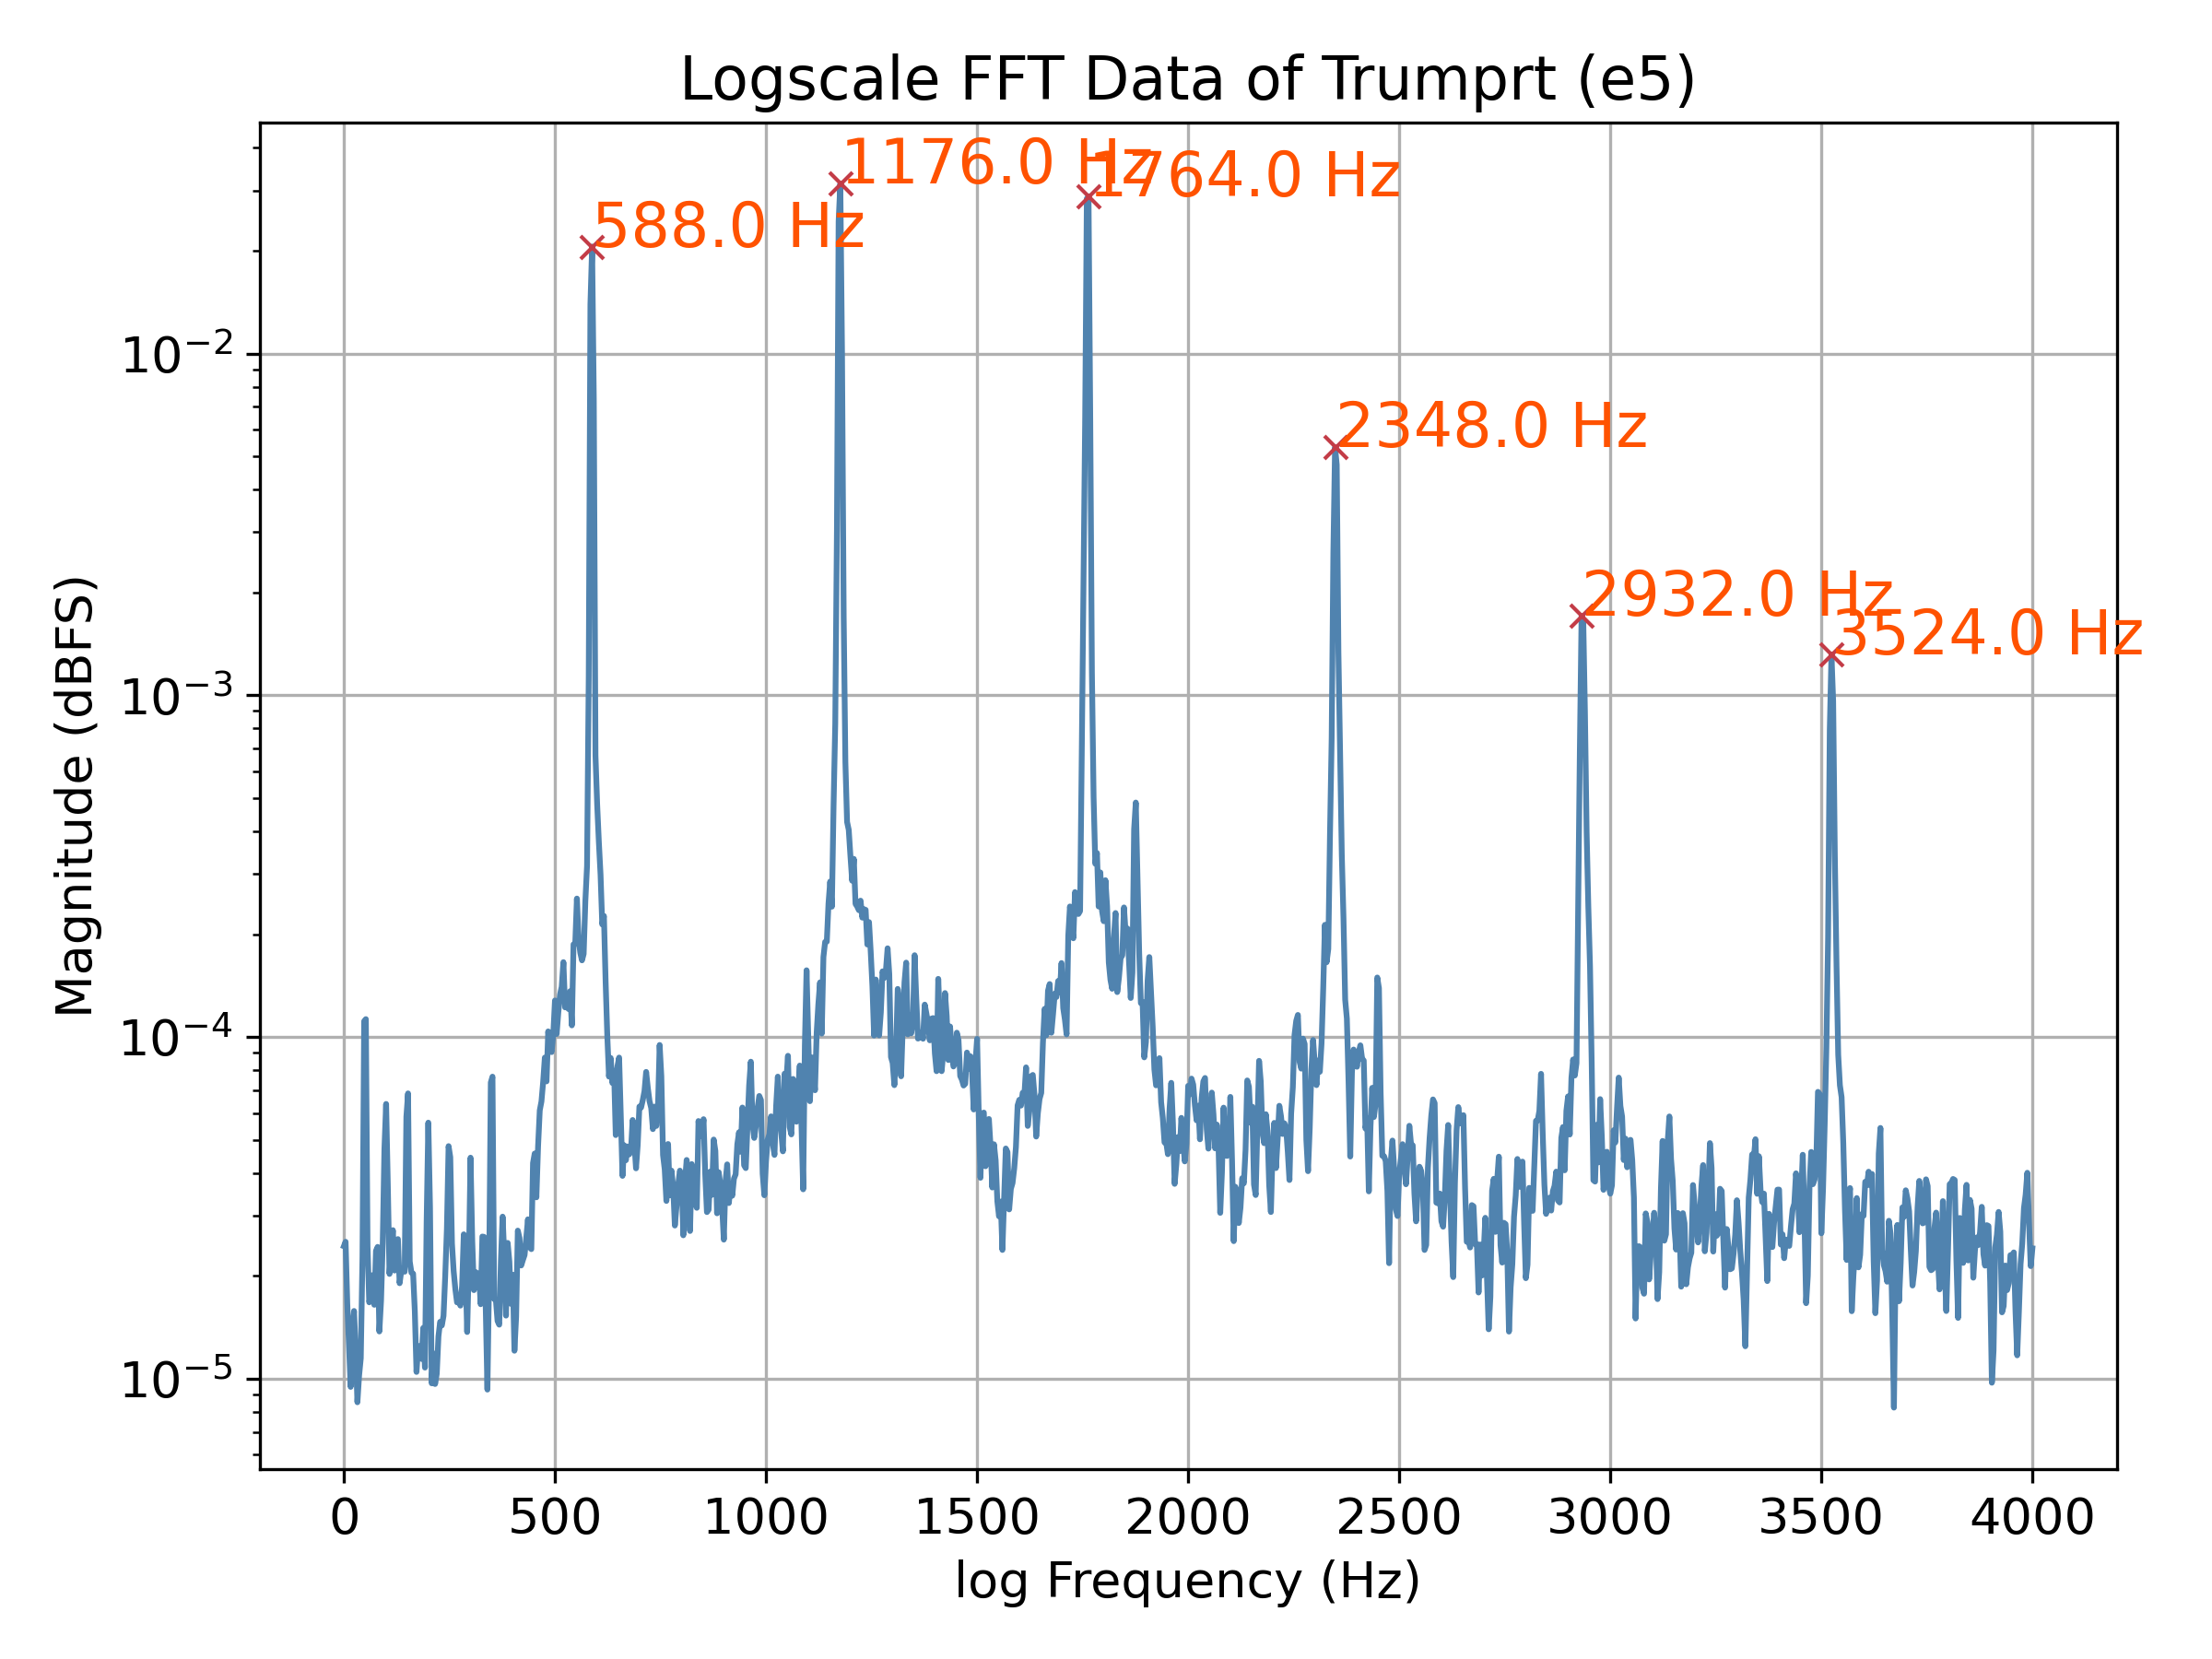
\includegraphics{/Users/kiloverse/Documents/物理学実験2/音のフーリエ解析/data/result_plot/4_fft_log_tram_e5.png}}}
          \caption{パンパイプE5音(y in logscale)}
        \end{minipage}
    \end{figure}
    \FloatBarrier

    最後に、楽器とは言えないかもしれないが、人の口笛のC6、D6、E6の周波数成分も測定した。
    \begin{figure}[htbp]
        \centering
        \begin{minipage}[b]{0.49\textwidth} % minipage 环境用于在同一行内并排放置内容,[b] 参数表示底部对齐,{0.5\textwidth} 设置 minipage 的宽度为页面宽度的一半
          \centering
          \fbox{\adjustbox{height=0.265\textheight,keepaspectratio}{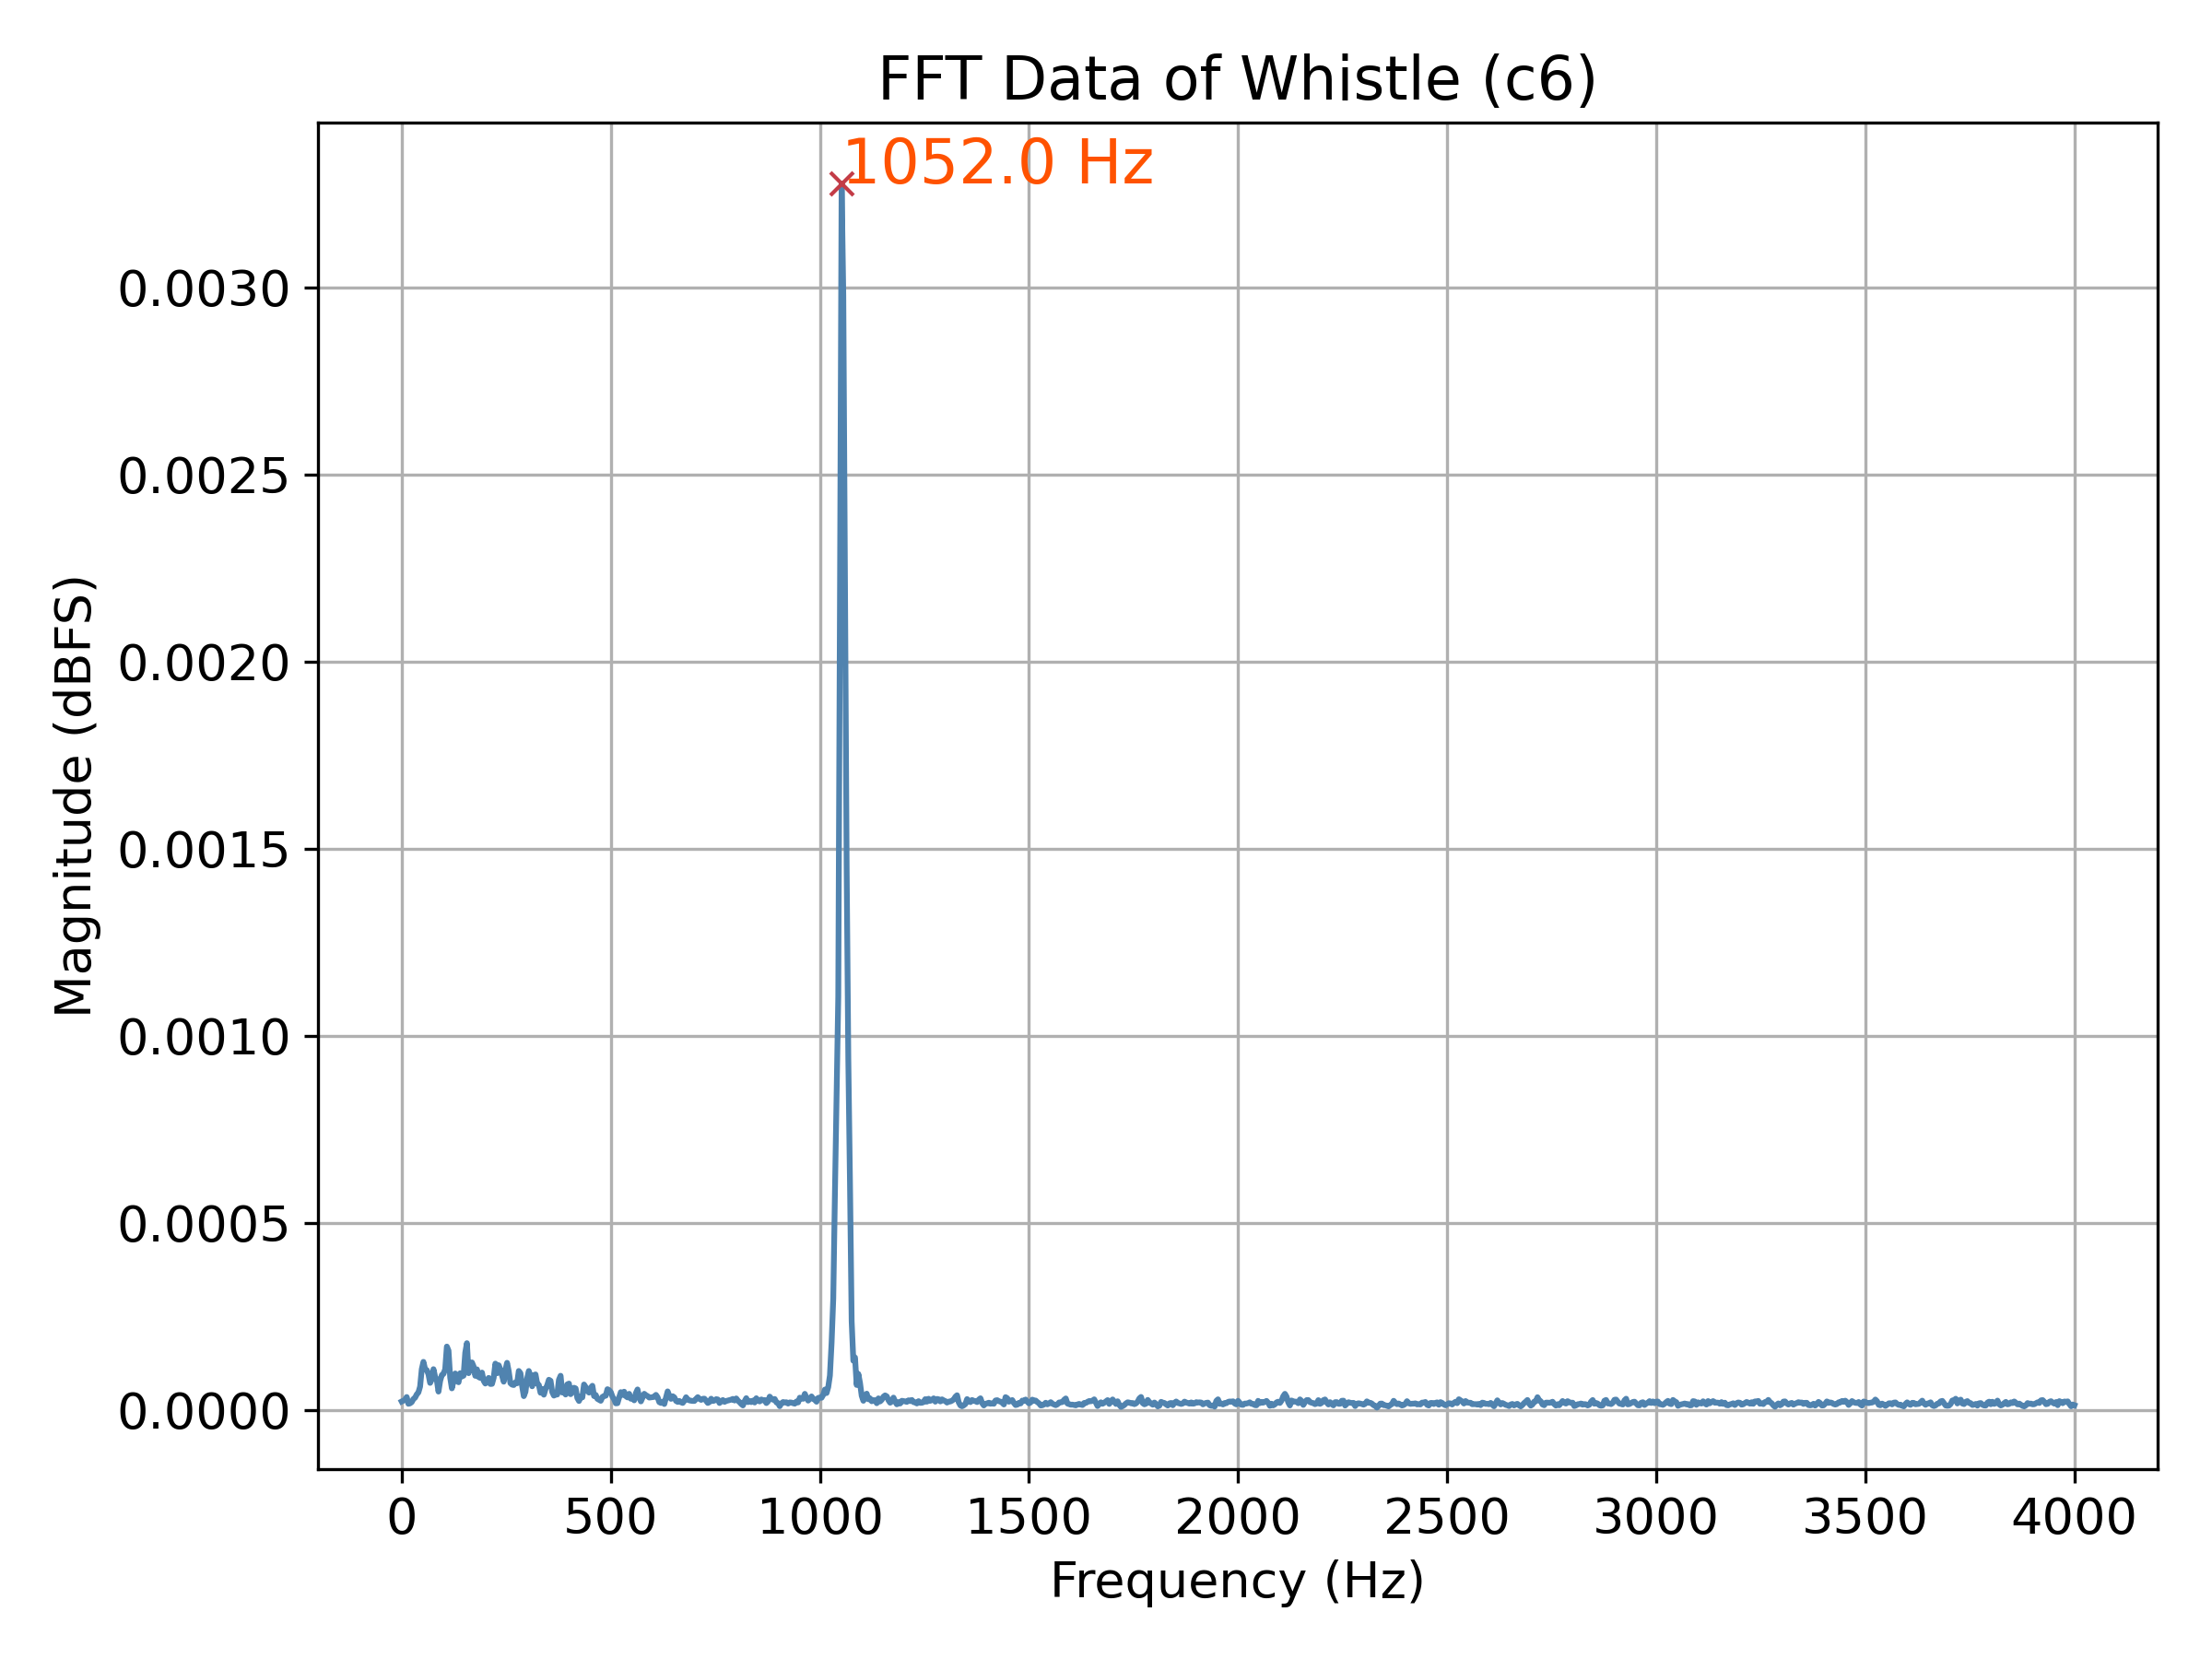
\includegraphics{/Users/kiloverse/Documents/物理学実験2/音のフーリエ解析/data/result_plot/4_fft_kuti_c6.png}}}
          \caption{口笛C6音}
        \end{minipage}% % 在两个 minipage 环境之间使用 % 符号来消除之间的空白
        \begin{minipage}[b]{0.49\textwidth}
          \centering
          \fbox{\adjustbox{height=0.265\textheight,keepaspectratio}{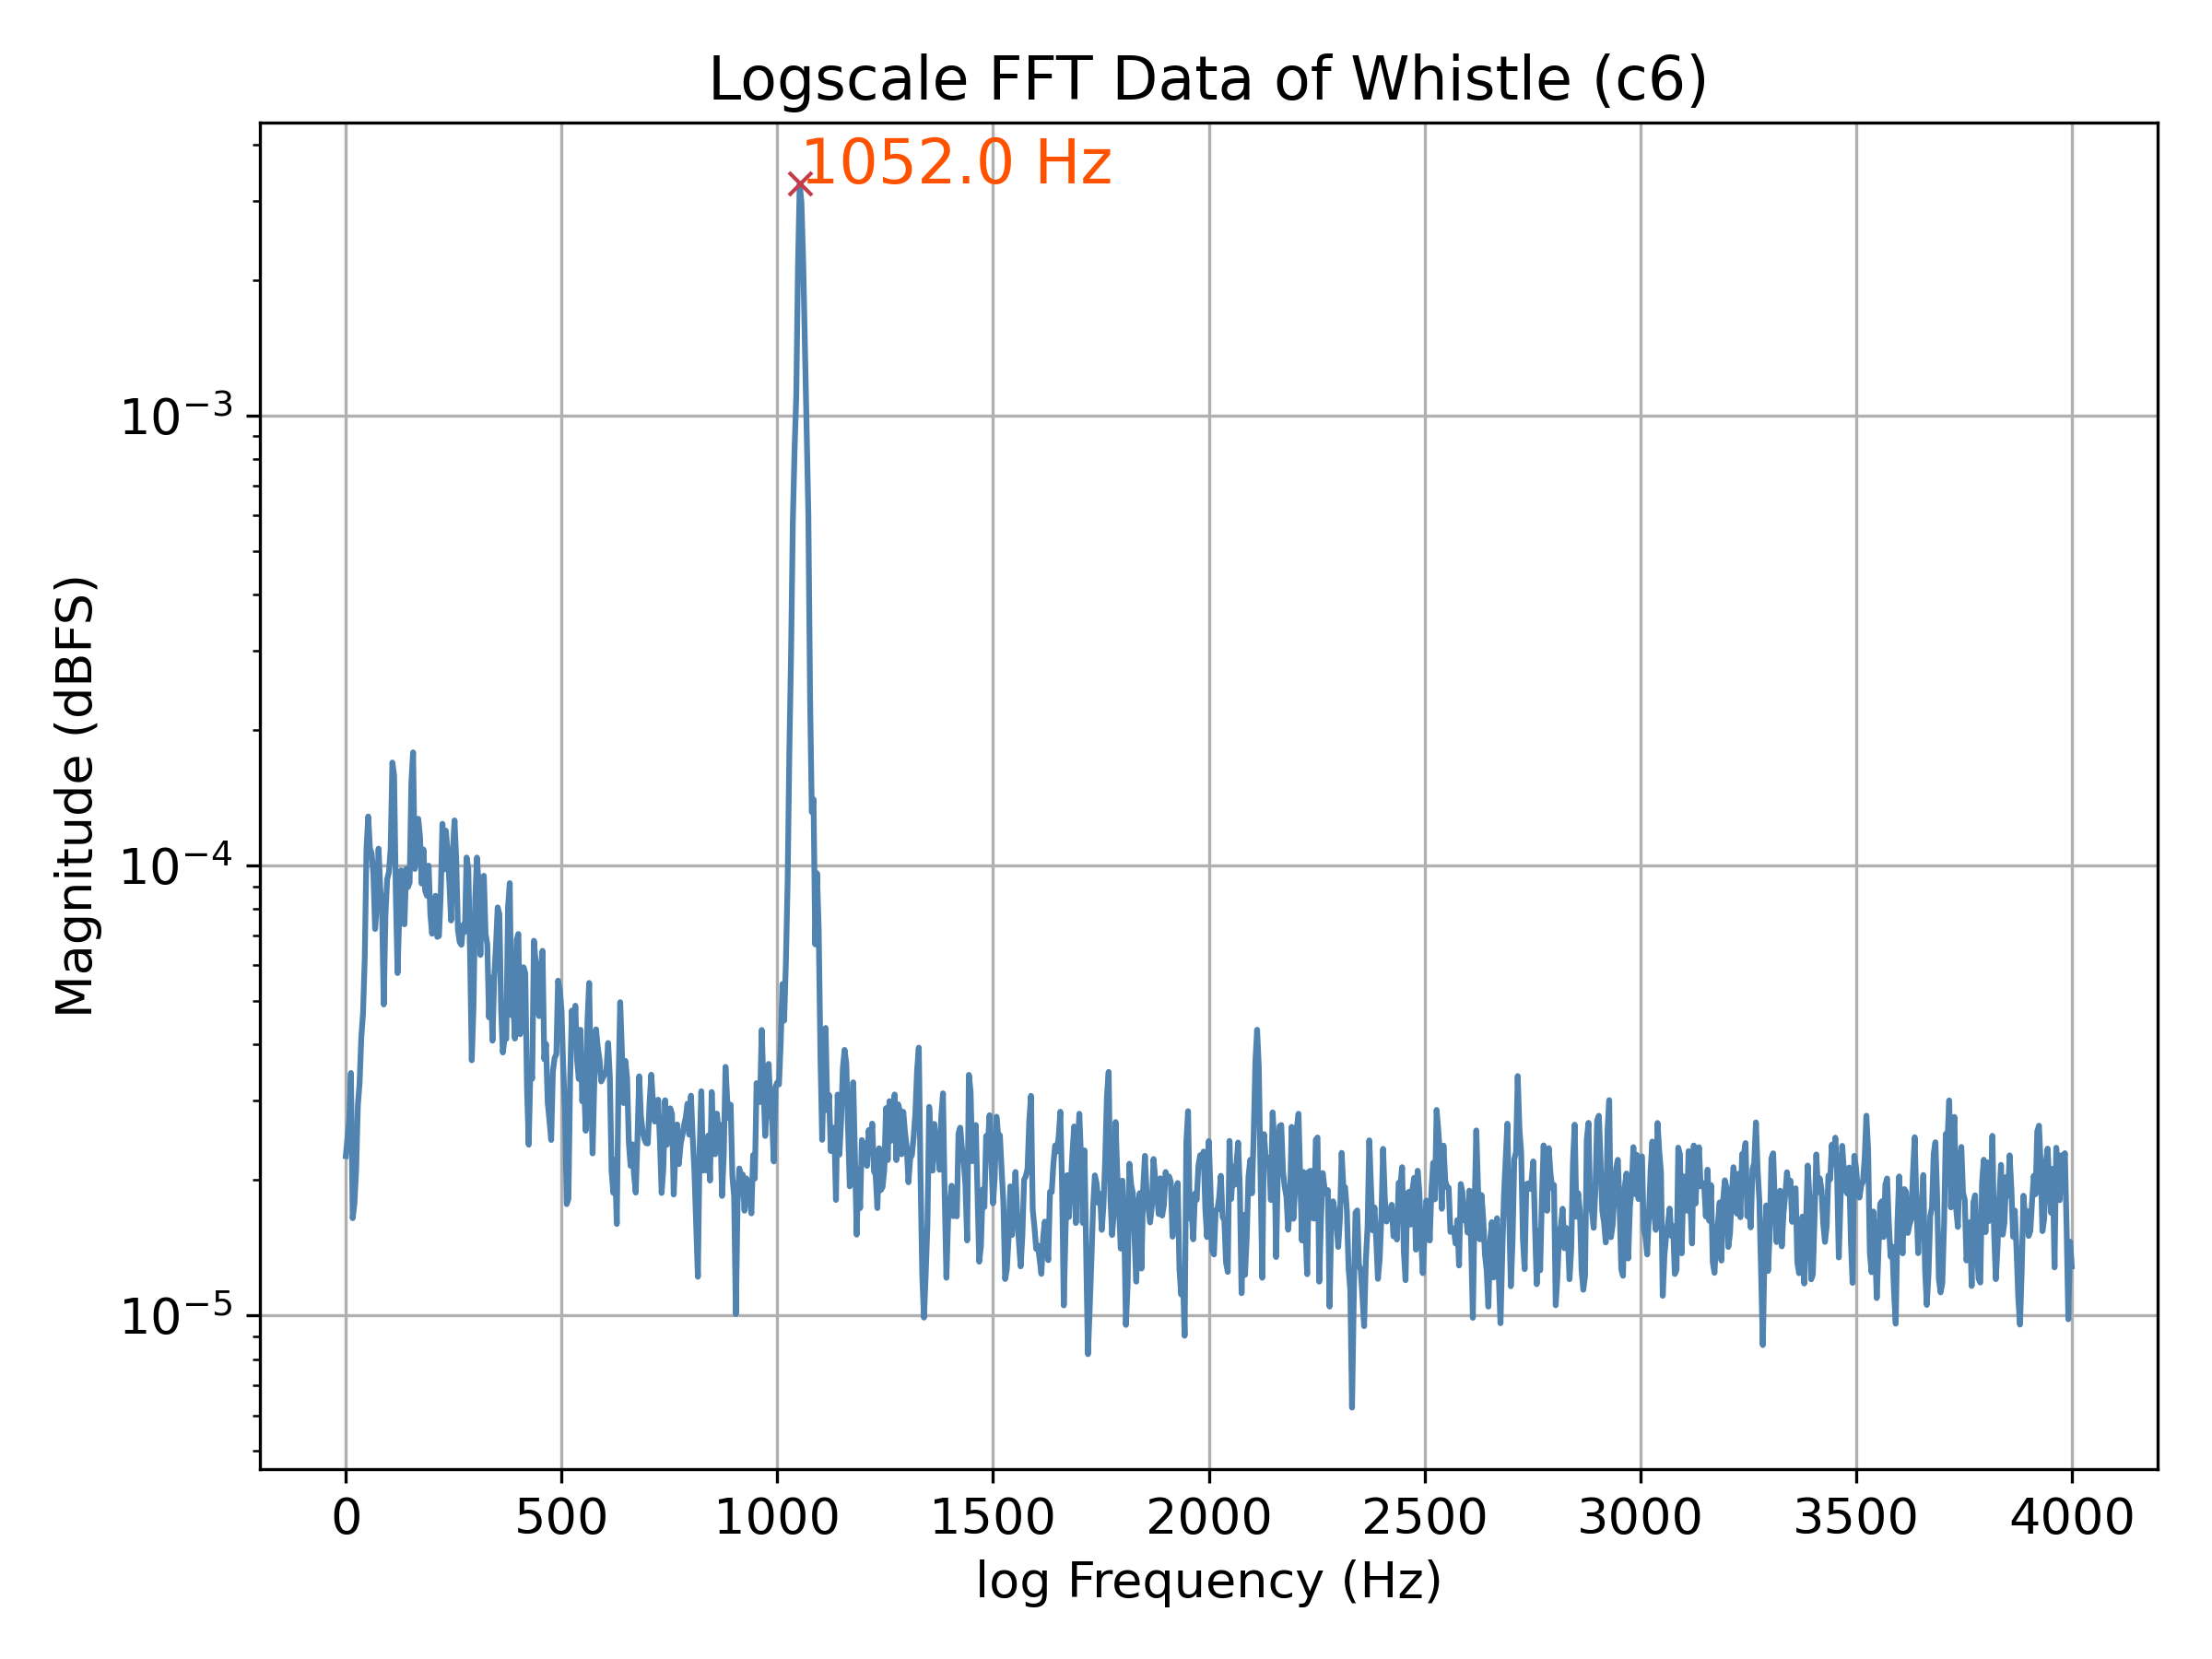
\includegraphics{/Users/kiloverse/Documents/物理学実験2/音のフーリエ解析/data/result_plot/4_fft_log_kuti_c6.png}}}
          \caption{口笛C6音(y in logscale)}
        \end{minipage}
    \end{figure}
    \begin{figure}[htbp]
        \centering
        \begin{minipage}[b]{0.49\textwidth} % minipage 环境用于在同一行内并排放置内容,[b] 参数表示底部对齐,{0.5\textwidth} 设置 minipage 的宽度为页面宽度的一半
          \centering
          \fbox{\adjustbox{height=0.265\textheight,keepaspectratio}{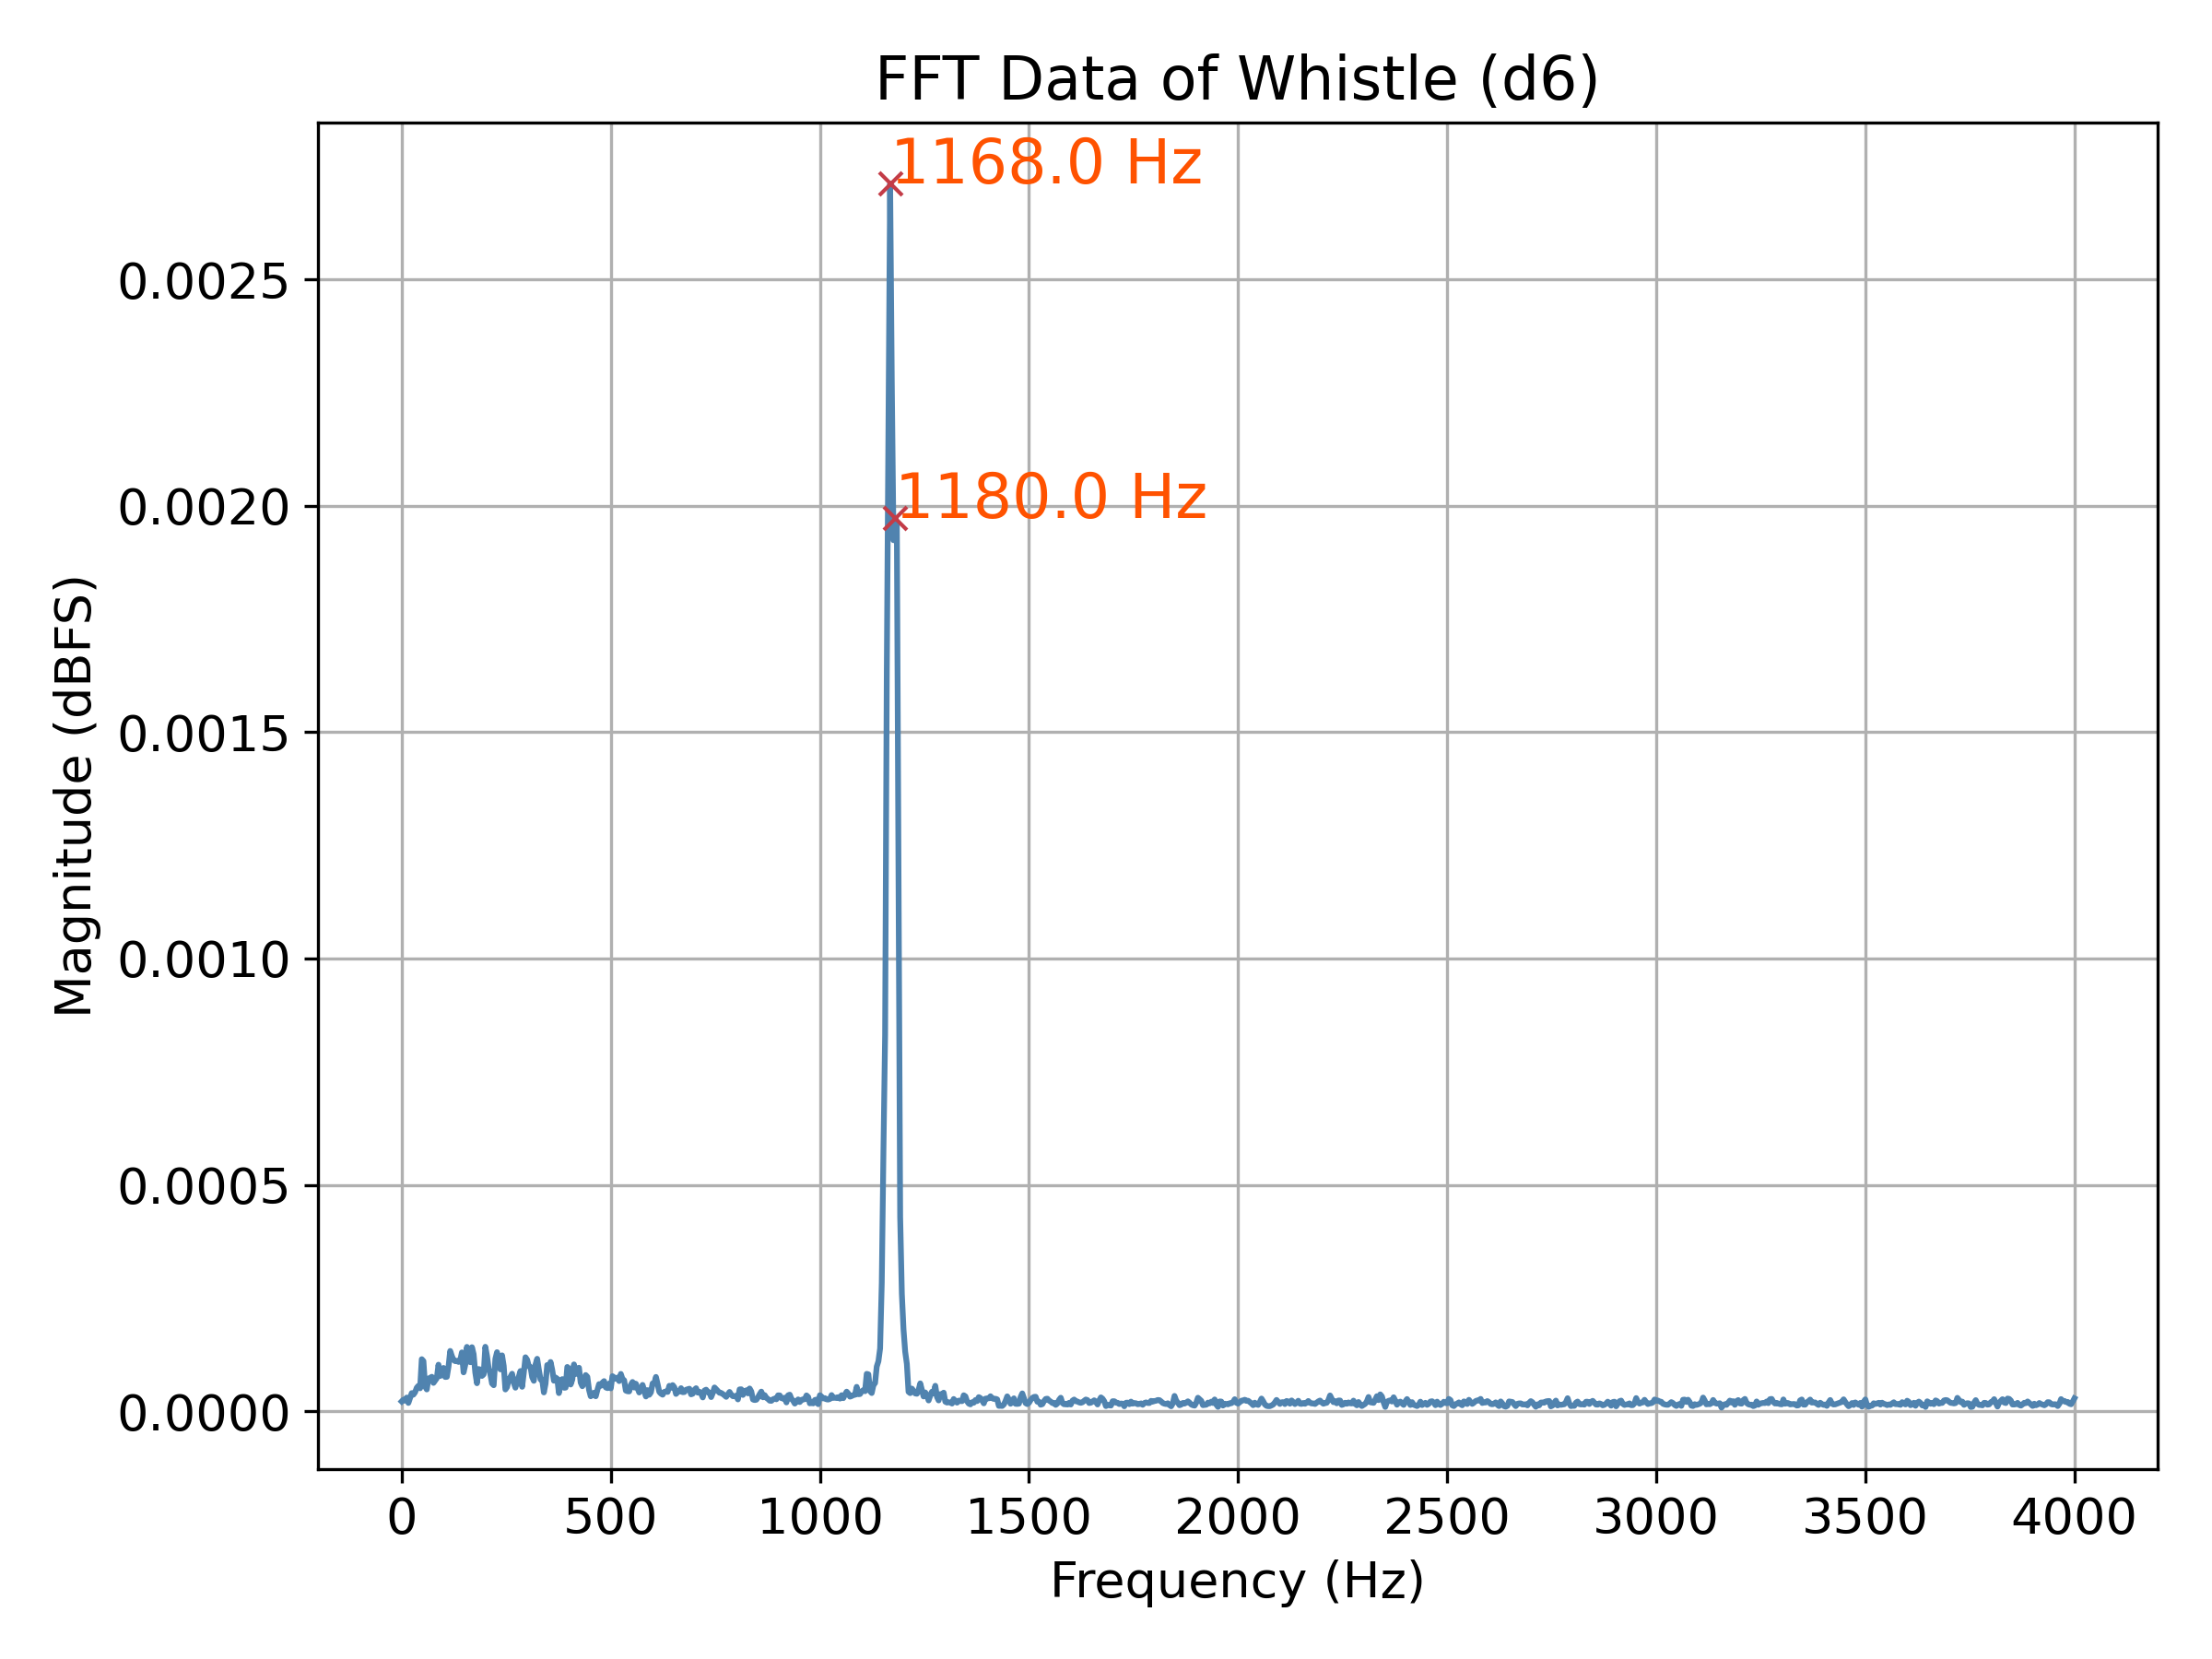
\includegraphics{/Users/kiloverse/Documents/物理学実験2/音のフーリエ解析/data/result_plot/4_fft_kuti_d6.png}}}
          \caption{口笛D6音}
        \end{minipage}% % 在两个 minipage 环境之间使用 % 符号来消除之间的空白
        \begin{minipage}[b]{0.49\textwidth}
          \centering
          \fbox{\adjustbox{height=0.265\textheight,keepaspectratio}{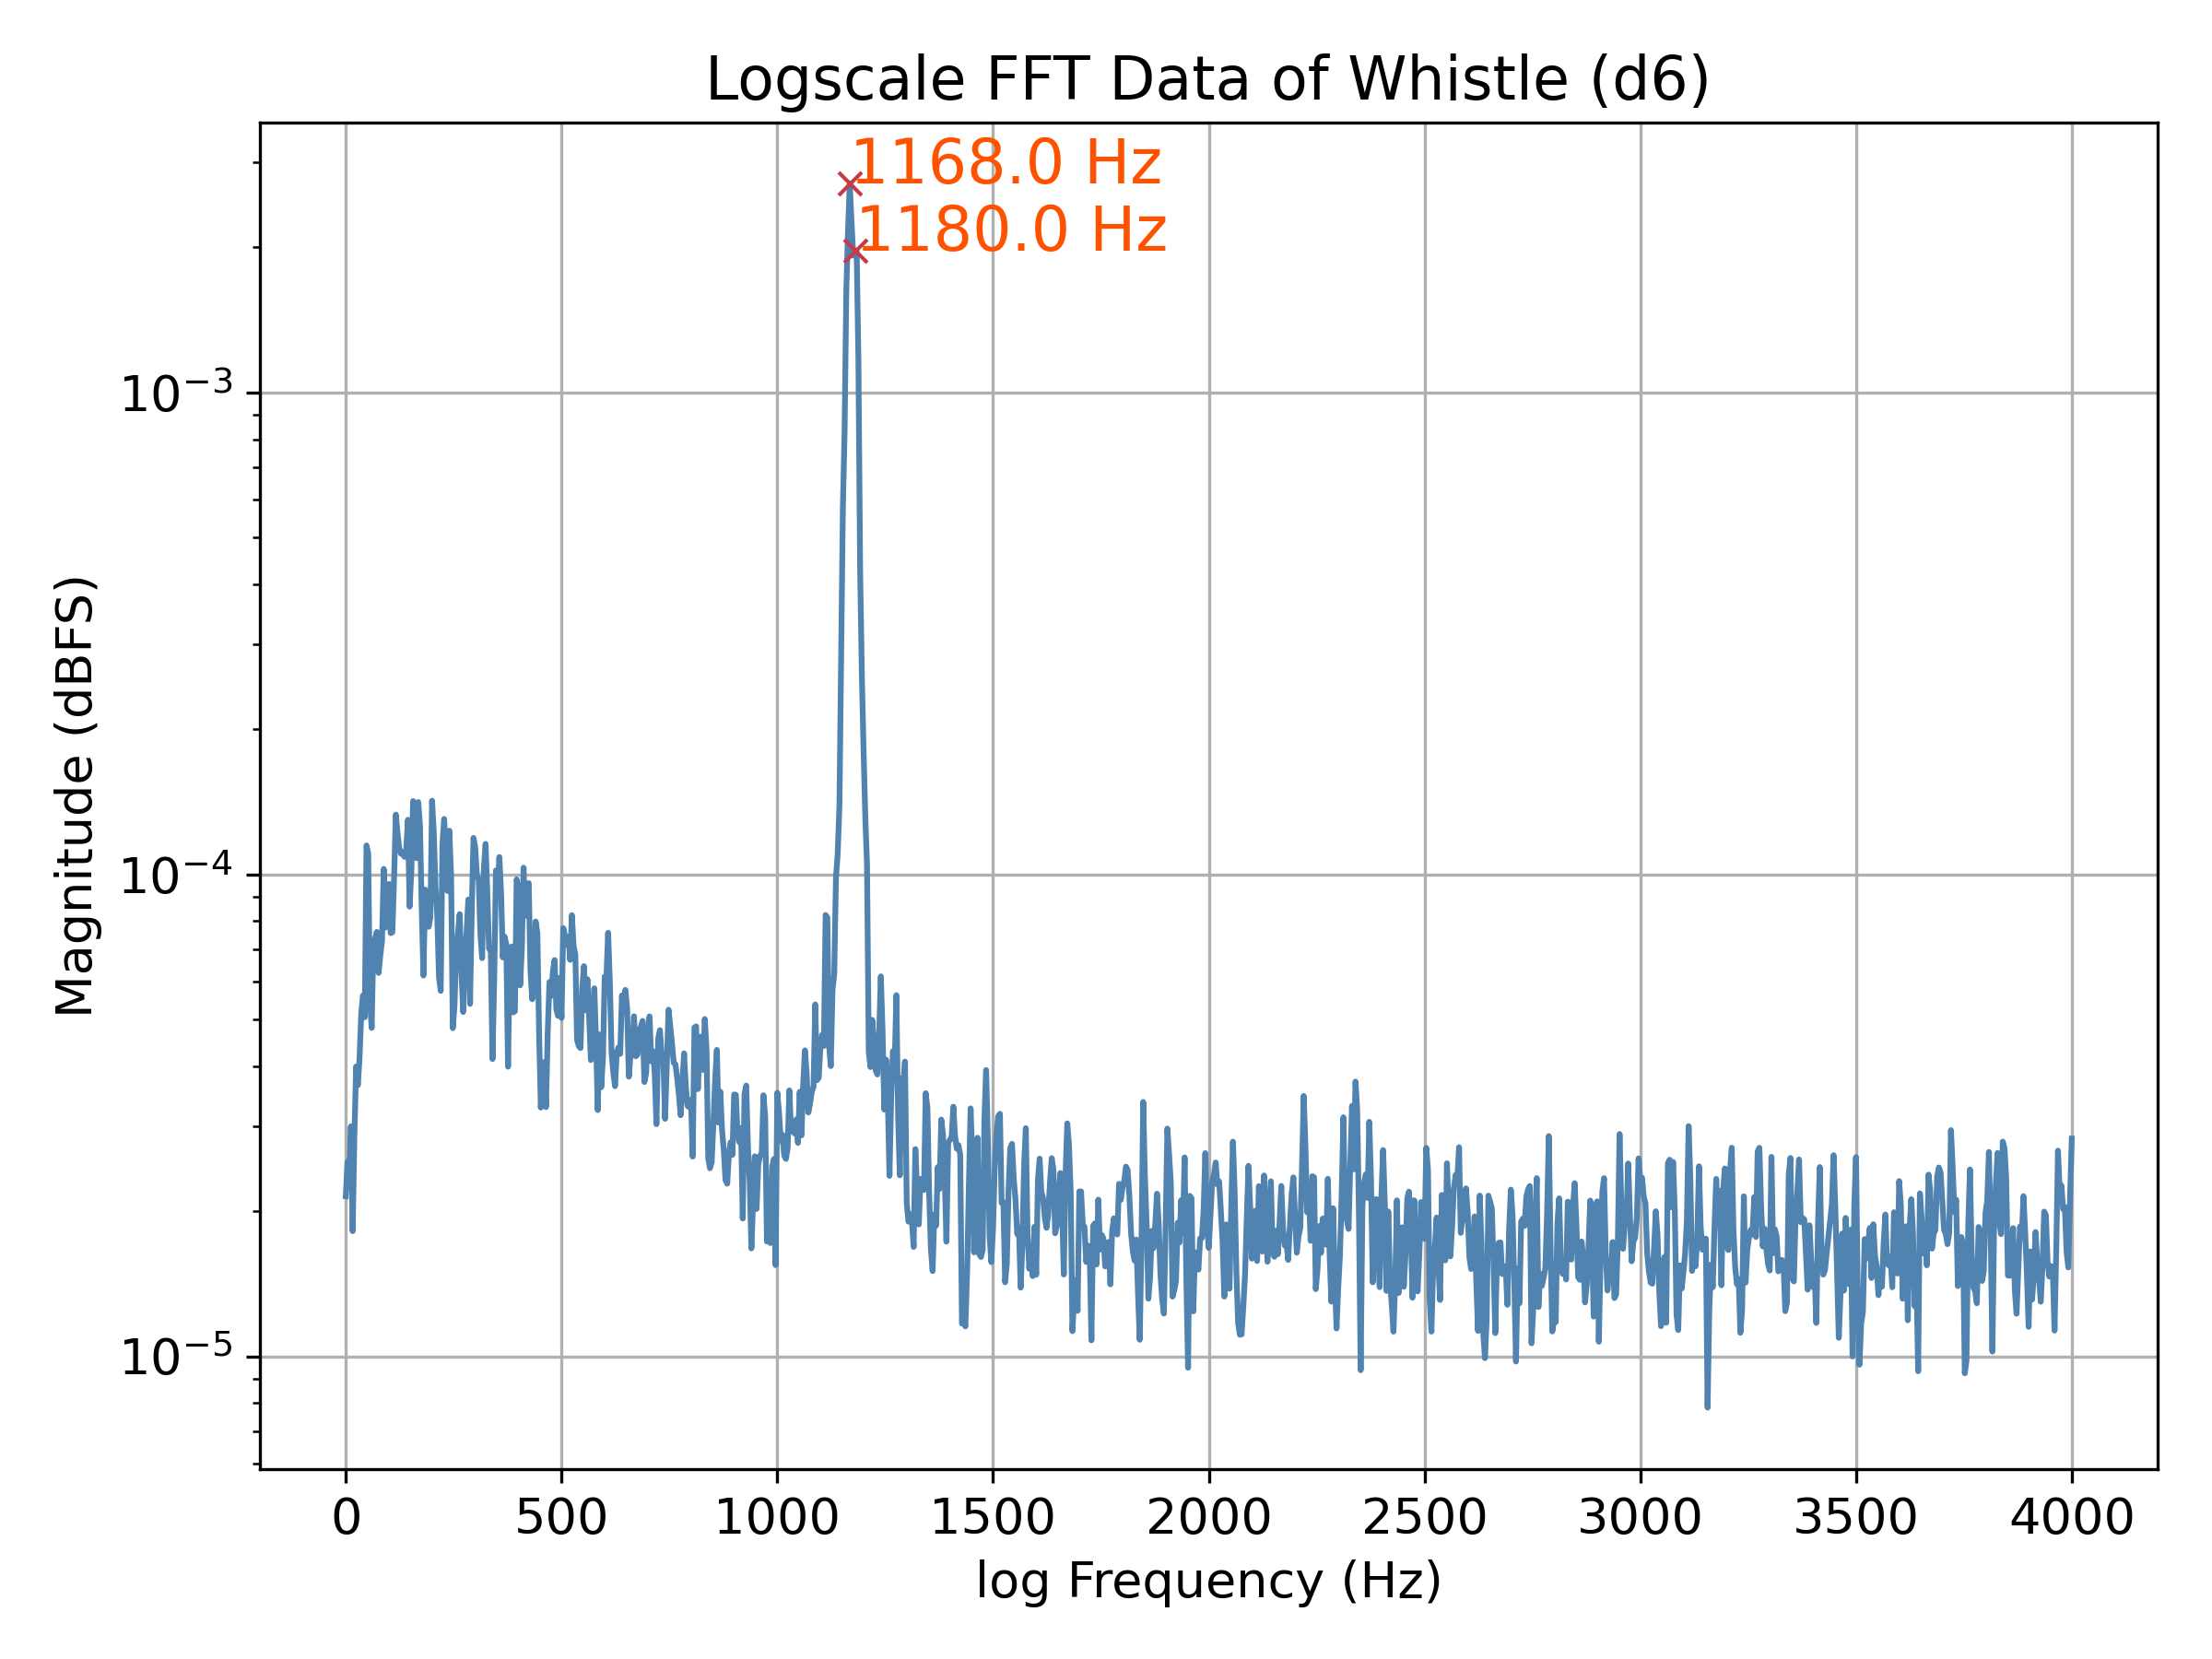
\includegraphics{/Users/kiloverse/Documents/物理学実験2/音のフーリエ解析/data/result_plot/4_fft_log_kuti_d6.png}}}
          \caption{口笛D6音y in logscale)}
        \end{minipage}
    \end{figure}
    \begin{figure}[htbp]
        \centering
        \begin{minipage}[b]{0.49\textwidth} % minipage 环境用于在同一行内并排放置内容,[b] 参数表示底部对齐,{0.5\textwidth} 设置 minipage 的宽度为页面宽度的一半
          \centering
          \fbox{\adjustbox{height=0.265\textheight,keepaspectratio}{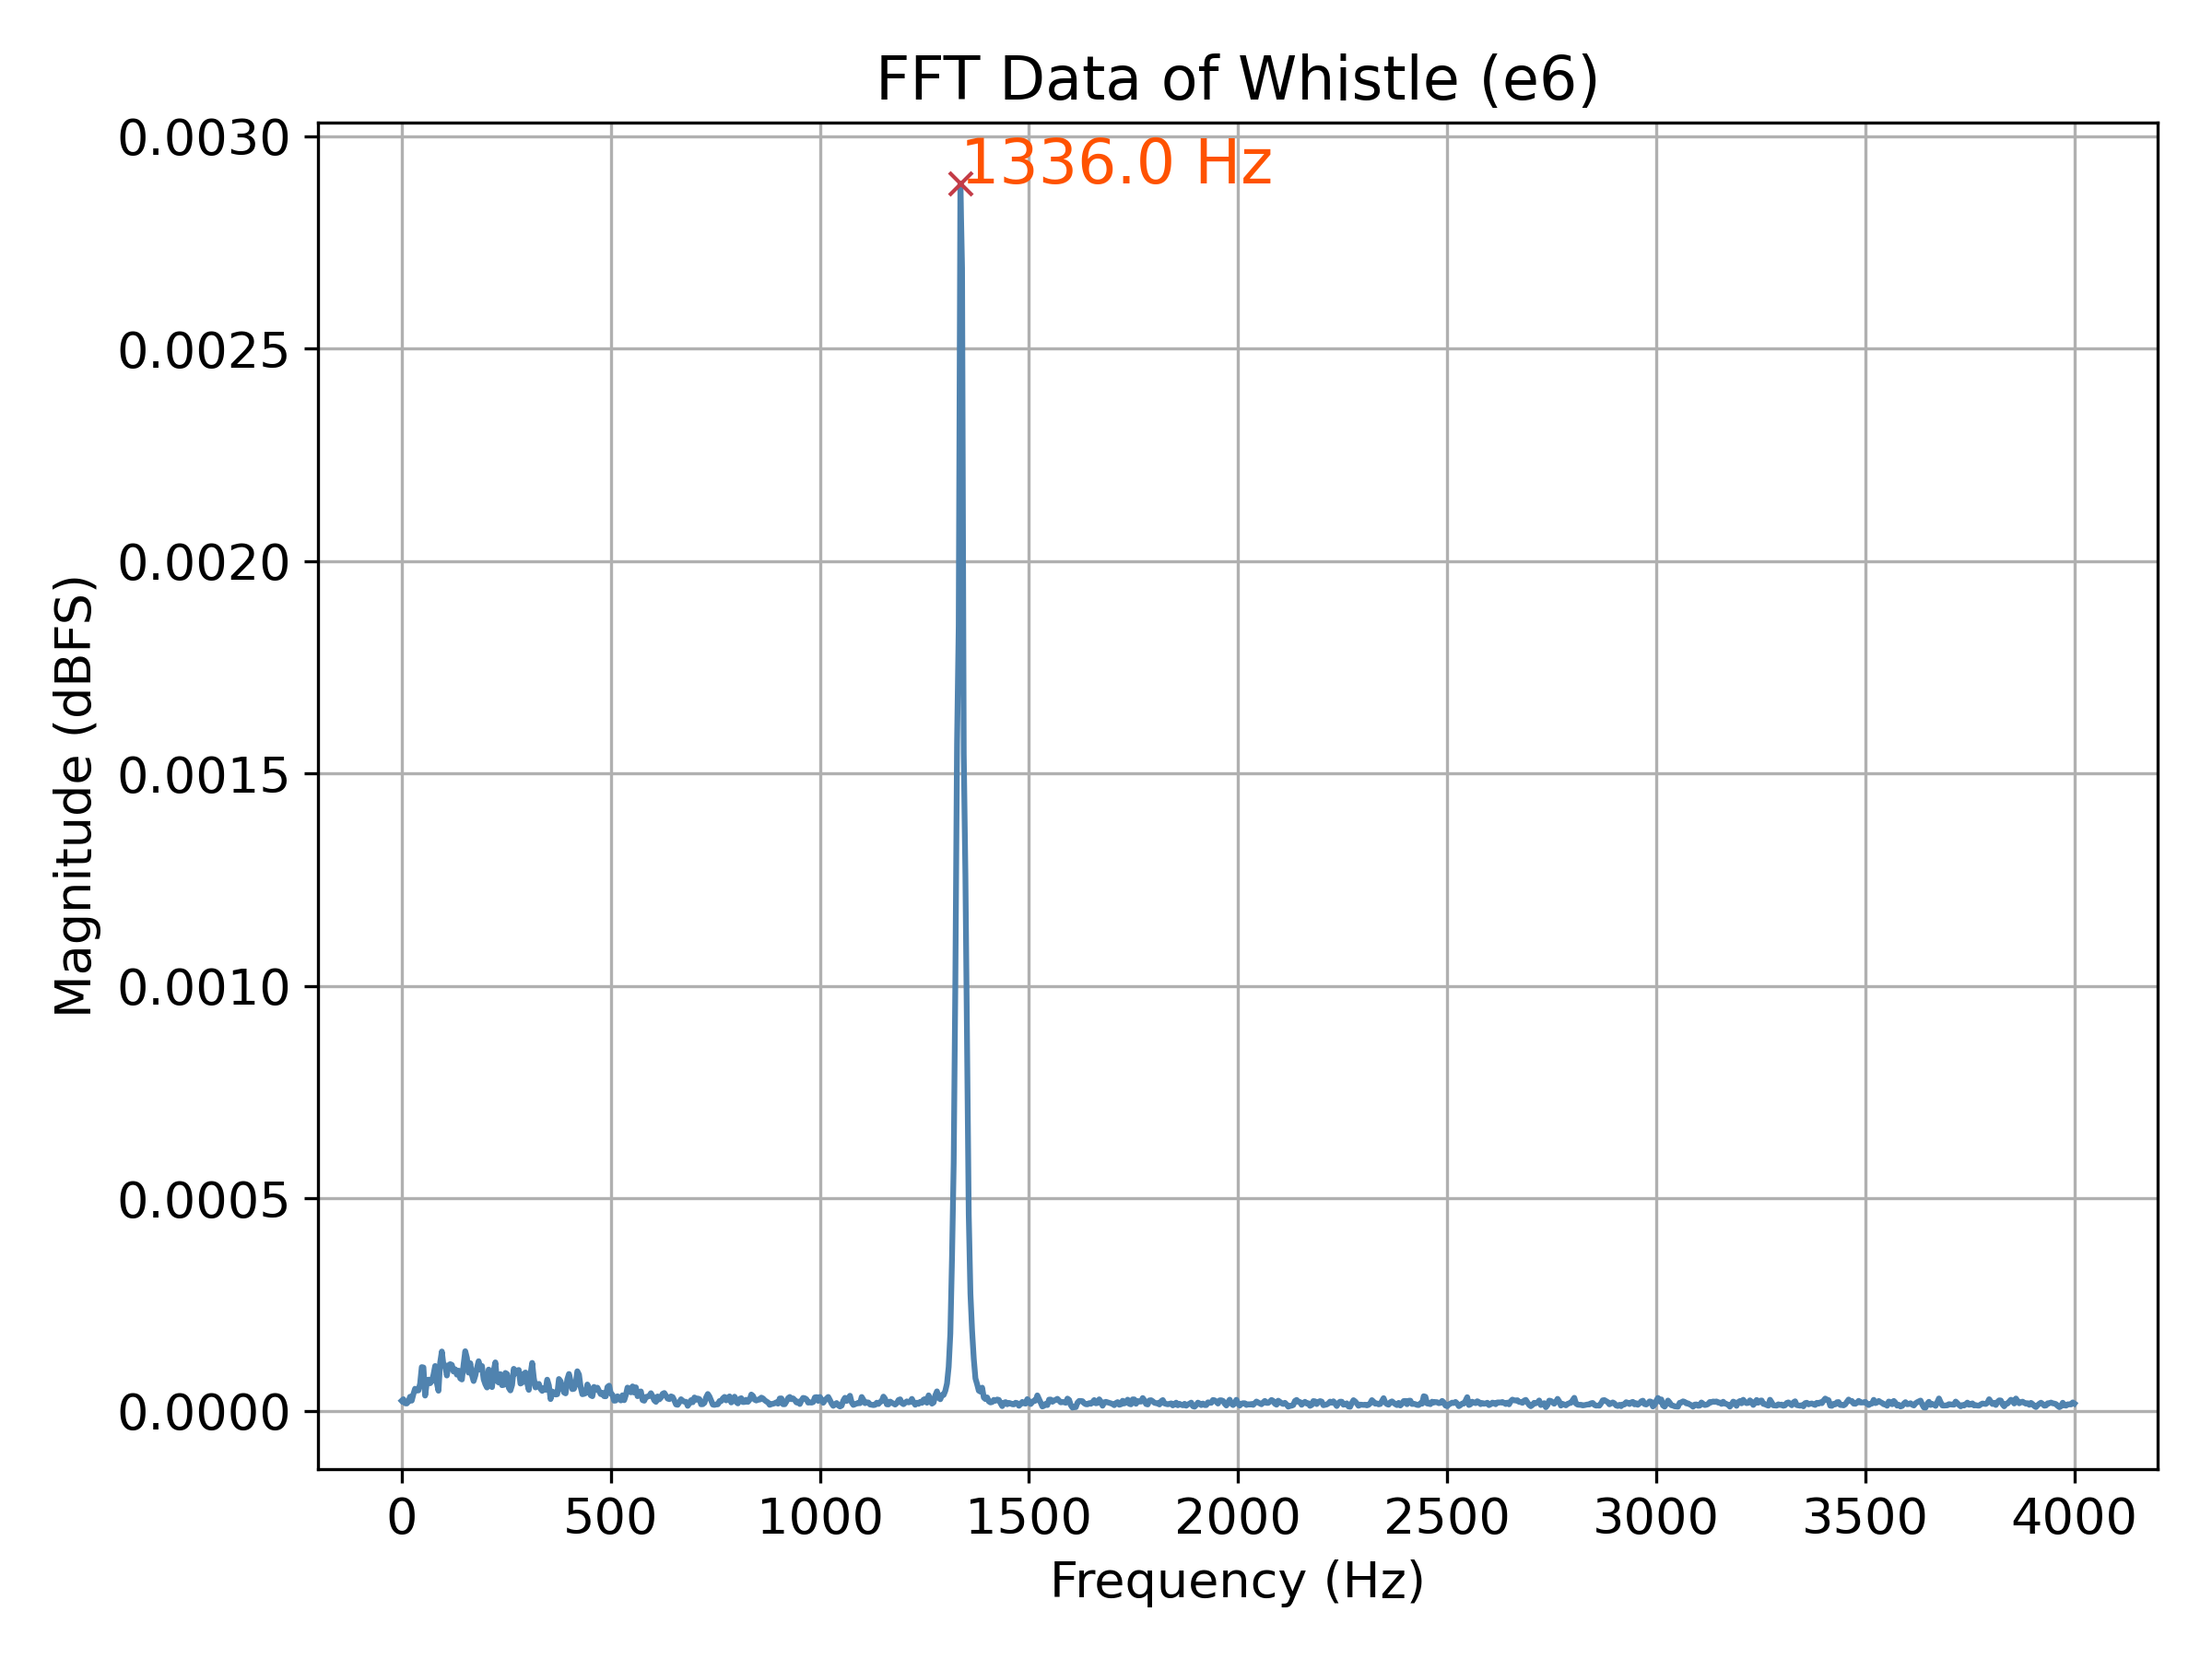
\includegraphics{/Users/kiloverse/Documents/物理学実験2/音のフーリエ解析/data/result_plot/4_fft_kuti_e6.png}}}
          \caption{口笛E6音}
        \end{minipage}% % 在两个 minipage 环境之间使用 % 符号来消除之间的空白
        \begin{minipage}[b]{0.49\textwidth}
          \centering
          \fbox{\adjustbox{height=0.265\textheight,keepaspectratio}{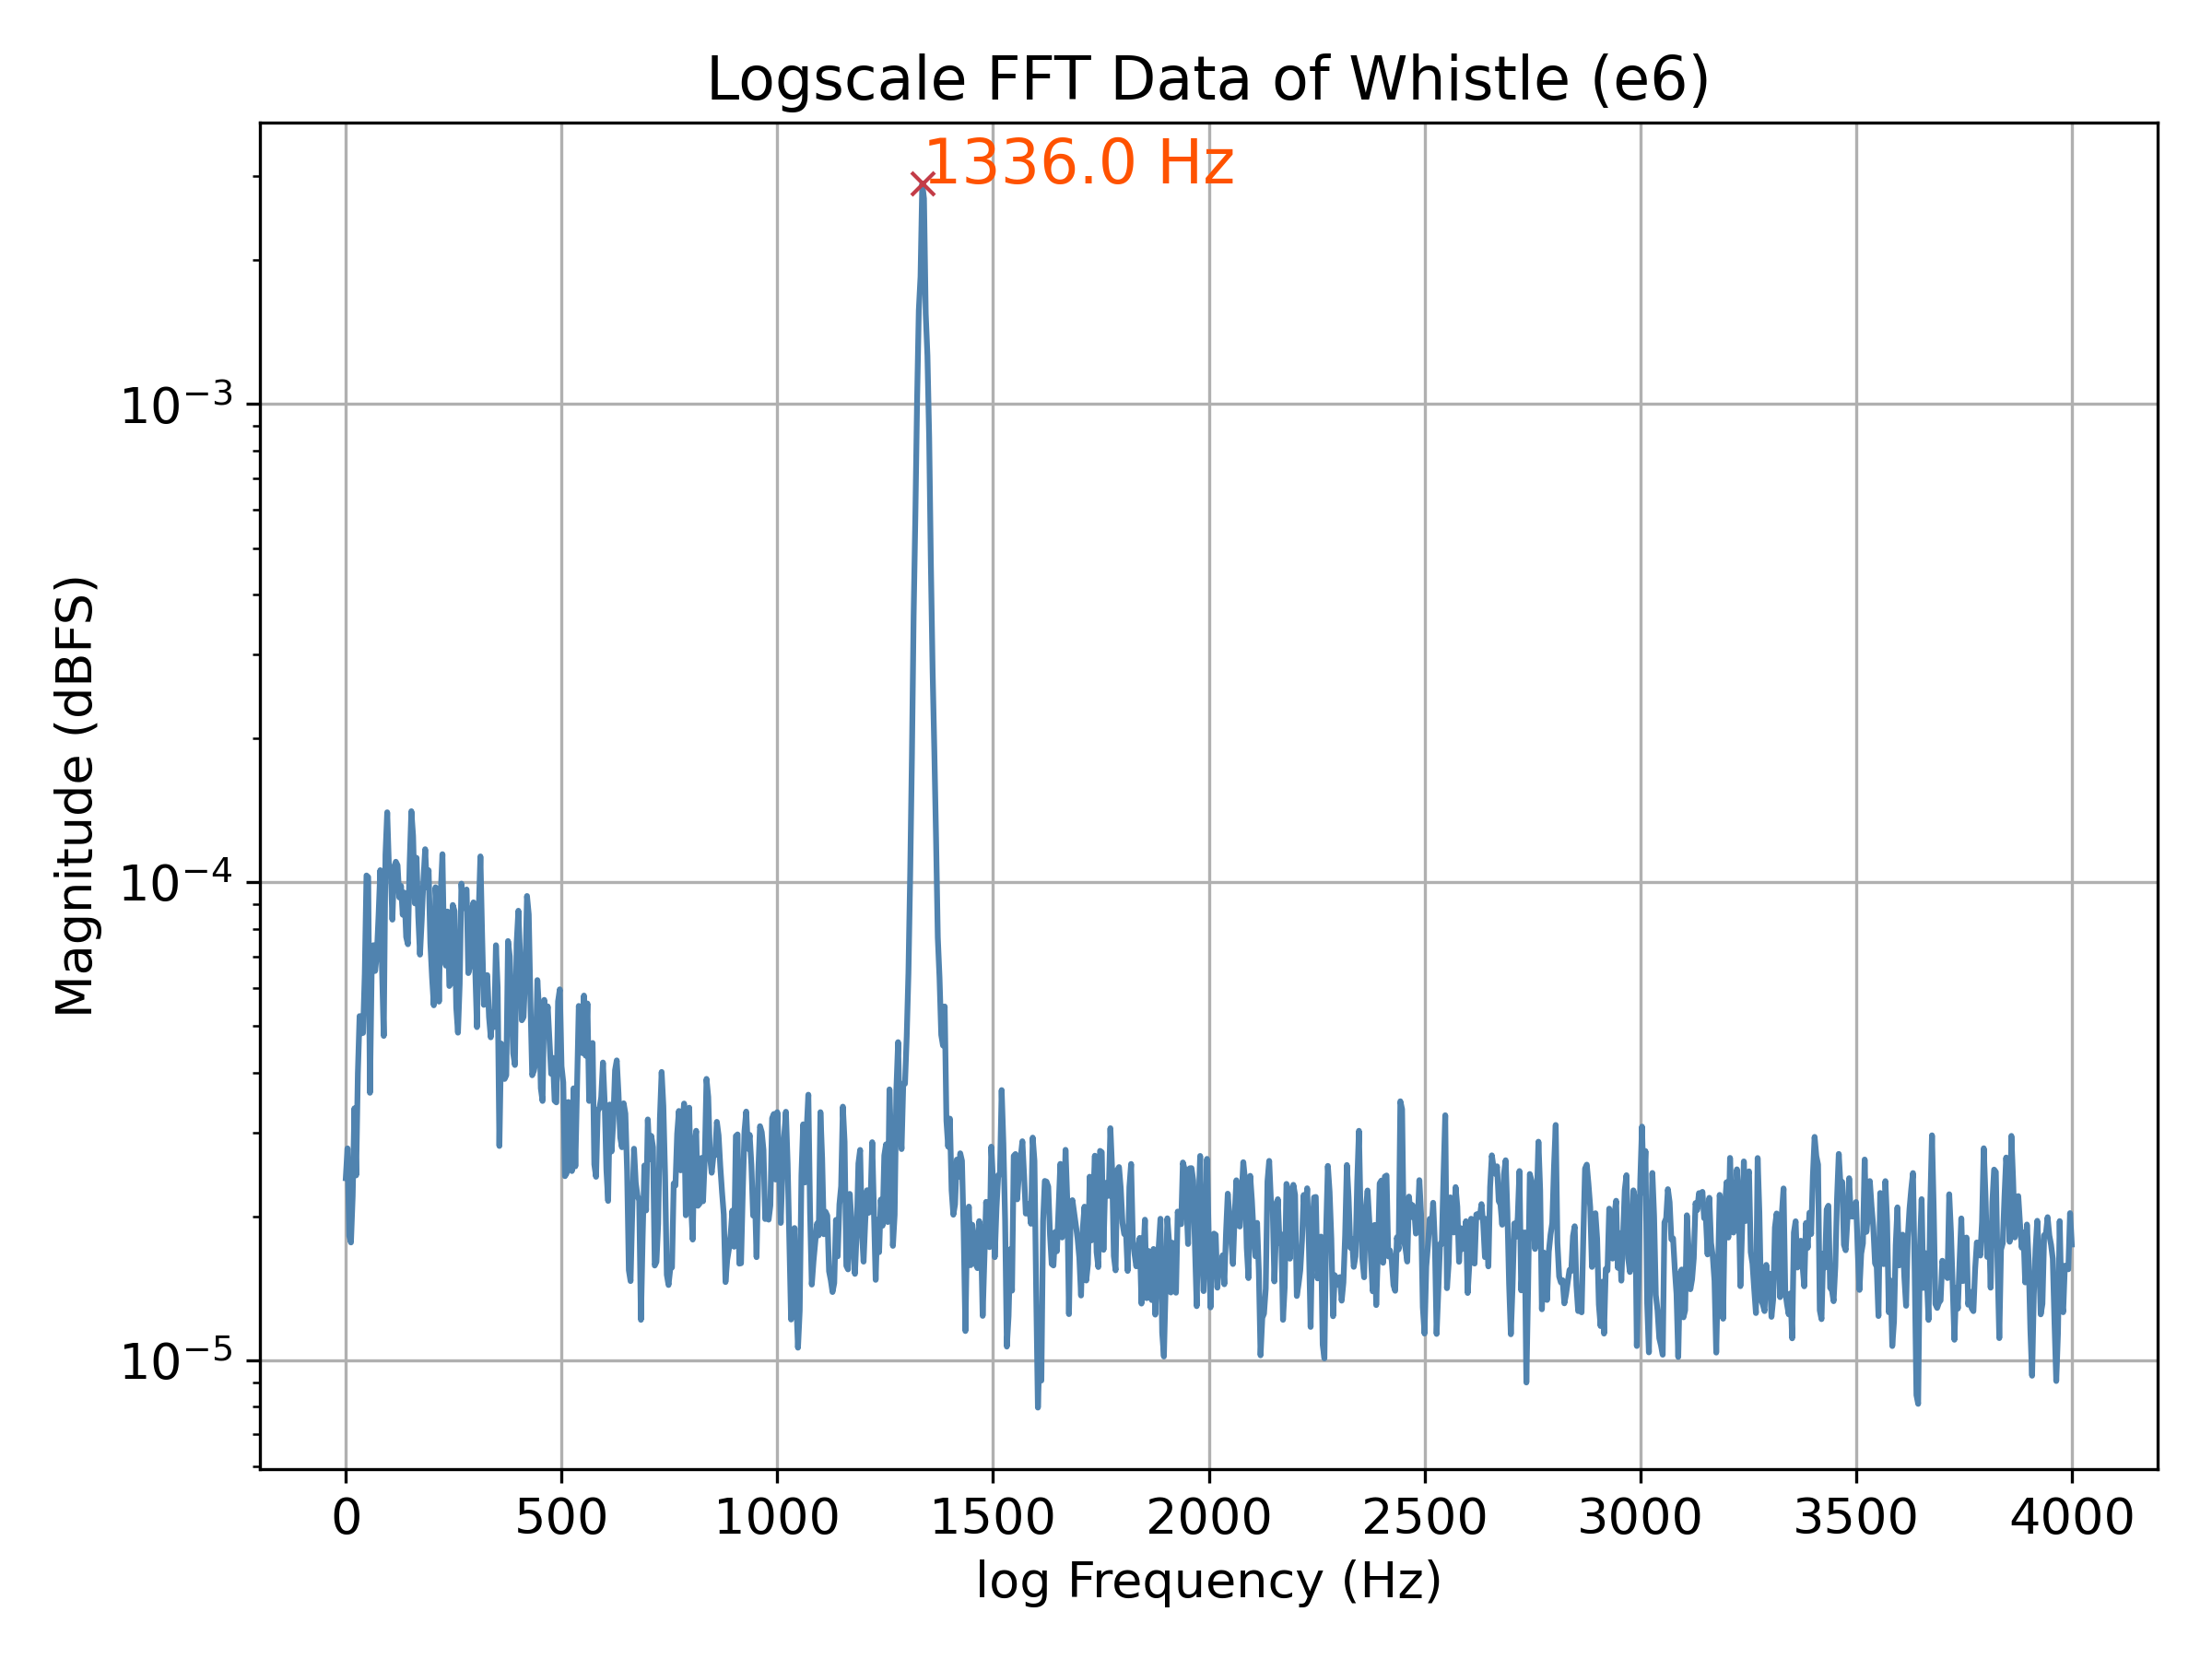
\includegraphics{/Users/kiloverse/Documents/物理学実験2/音のフーリエ解析/data/result_plot/4_fft_log_kuti_e6.png}}}
          \caption{口笛E6音(y in logscale)}
        \end{minipage}
    \end{figure}
    \FloatBarrier
    \subsubsection*{結果の解析}
    \begin{itemize}[label={--}]
        \item パンパイプでは、基本振動が主導的で、ハーモニクスはほとんど観察されない。このため、パンパイプの音色は非常に純粋でクリアだと感じられた。
        \item トランペットでは、高いハーモニクスの内容が豊富であるため、音色が豊かで力強い。トランペットの音は華やかで、音楽的な表現が広がる。
        \item 口笛では、基本振動のみが発生し、他のハーモニクスはほとんど見られない。そのため、音色は非常にシンプルである。
        \item 平均律においては、オクターブ(8度)間の周波数比が常に2:1となる。ここで、C4の基本振動数は約260Hz、C5の基本振動数は約524Hz、C6の基本振動数は約1048Hzで、平均律の基本原理と一致している。
    \end{itemize}
\end{spacing}

\subsubsection{考察8:振動原理と音色}
\begin{spacing}{1.2}
    各楽器の音色はその振動原理および周波数成分によって、音色が決まる。以下に、各楽器の音の生成、倍音の特性、および音色との関連についての考察をまとめた。
    \paragraph*{パンパイプ:}
    パンパイプの音は、管の長さに応じた空気の柱の振動によって生成される。プレイヤーが管に向かって息を吹き込むことで、音が発生する。この楽器は基本振動が主導的であり、倍音はほとんど存在しないため、音色は非常にクリアで純粋である。そのため、音色は透明感があり、穏やかで優しい印象を与える。
    \begin{figure}[ht] % 选项 [htbp] 代表位置优先级, “here, top, bottom, page” 分别表示:此处、页顶、页底、单独一页
        \centering
        \fbox{\adjincludegraphics[width=0.4\textwidth]{/Users/kiloverse/Documents/物理学実験2/音のフーリエ解析/data/report_figs/パンパイパ.png}}
        \caption{パンパイパ}
    \end{figure}
    \FloatBarrier
    \paragraph*{トランペット:} 
    トランペットの音は、プレイヤーがマウスピースに息を吹き込むことで唇の振動が空気の柱を振動させ、楽器全体で共鳴することにより生成される。トランペットは多くの倍音を生じさせる金管楽器であるため、音色は豊かで、「ブライト」で「パワフル」と感じられる。高倍音が強調されることにより、明るく力強い響きが特徴となる。
    \begin{figure}[ht] % 选项 [htbp] 代表位置优先级, “here, top, bottom, page” 分别表示:此处、页顶、页底、单独一页
        \centering
        \fbox{\adjincludegraphics[width=0.4\textwidth]{/Users/kiloverse/Documents/物理学実験2/音のフーリエ解析/data/report_figs/トランペット.png}}
        \caption{トランペット}
    \end{figure}
    \FloatBarrier
    \paragraph*{口笛:}
    口笛では、プレイヤーの唇の間で空気が振動し、音が生じる。この楽器は非常にシンプルな音源であるため、倍音が存在せず、基本周波数のみが現れる。そのため、口笛の音色は非常にシンプルでクリアであり、基本周波数のみに依存するため、独特の清潔感がある。
    \paragraph*{ピアノ:}
    ピアノの音は、ハンマーが弦を叩くことによって生成される。このとき、弦の振動が共鳴板を通じて音が増幅される。ピアノの弦は、基本周波数に加えて多くの倍音を生成し、これらの倍音は音色に富み複雑さを与える。そのため、ピアノの音色は「ウォーム」で「リッチ」と感じられる。
    \paragraph*{ギター:}
    ギターの音は、プレイヤーが弦を指で弾くことにより生成される。弦の振動がギターのボディで共鳴し、音が増幅される。ギターは、弦の長さや張力によって基本周波数と多数の倍音が生成されるため、音色に深みと温かみが感じられる。
\end{spacing}

\subsubsection{考察9:気柱の奇数倍振動}
\begin{spacing}{1.2}
    図59で観察されたように、パンパイプで奇数倍振動しか起こらなかった現象がある。これはパンパイプ内の気柱の振動に原因がある。
    \begin{figure}[ht] % 选项 [htbp] 代表位置优先级, “here, top, bottom, page” 分别表示:此处、页顶、页底、单独一页
        \centering
        \fbox{\adjincludegraphics[width=0.3\textwidth]{/Users/kiloverse/Documents/物理学実験2/音のフーリエ解析/data/report_figs/閉管の奇数倍振動.png}}
        \caption{閉管の奇数倍振動}
    \end{figure}
    \FloatBarrier
    パンパイパの一端が塞がれた閉管で、各管は異なる長さを持ち、それぞれ異なる音程を出す。
    開口端は空気分子が自由に動けるため、定常波の腹となる。
    閉口端では空気分子が動けず、固定端として振動することで、定常波の節となる。
    気柱の波長は以下の式で表される:
    \[
    \lambda = \frac{4L}{2n-1}
    \]
    \begin{center}
        ($\lambda$: 波長, $L$: 管の長さ, $n=1, 3, 5, \ldots$)
    \end{center}
    したがって、パンパイプでは、管の長さと開口部の形状によって、奇数の整数倍($2n-1$)の振動のみが発生する。
\end{spacing}

% 6、実験結論%%%%%%%%%%%%%%%%%%%%%%%%%%%%%%%%%%%%%%%%%%%%%%%%
\section{実験結論}
\begin{enumerate}[label=\arabic*), before=\begin{spacing}{1.2}, after=\end{spacing}] % \arabic阿拉伯数字,\roman小写罗马数字,\Roman,\alph小写字母,\Alph,“*”之后添加自己喜欢的序号后样式, 如1.添加“.”,1)添加“)”;利用{spacing}自定义\item内的行间距
    \item \textbf{実験1}:母音の特性は、それぞれの累積スペクトルや周波数振幅比率によって明らかになり、高調波の特徴から識別することができることが確認された。
    \item \textbf{実験2}:フーリエ変換を用いて音の解析を行うことによって、周波数のスペクトルから和音を構成する音の識別が可能であることが明らかになった。和音はその構成音の周波数成分が複合的に表れ、特定の和音に特有のスペクトルパターンを形成する。
    \item \textbf{実験3}:フーリエ級数展開を用いて様々な特徴的な波形を再現することにより、フーリエ級数展開の特性と各波形の基本的な調和成分が理解された。正弦波、矩形波、ノコギリ波、三角波がそれぞれどのようにしてその特徴的な形状を生成しているかが示された。
    \item \textbf{実験4}:弦楽器では通常の奏法とハーモニクス奏法が音の生成にどのように影響するかが詳しく分析され、異なる楽器が持つユニークな倍音構造と音色が調査された。
\end{enumerate}
\begin{spacing}{1.2}
    以上により、物理数学で学習したフーリエ解析を、音を素材として実際の実験と感覚及び身近な例を通じて体得することができた。
    音波を時間ドメインと周波数ドメインで観察することにより、物理量の異なる見え方や音の性質を理解できた。
\end{spacing}

\newpage
% 参考文献 %%%%%%%%%%%%%%%%%%%%%%%%%%%%%%%%%%%%%%%%%%%%%%%%%%
\section*{参考文献}
\addcontentsline{toc}{section}{参考文献} % 将 参考文献 添加到目录中
\begin{spacing}{1.4}
    \noindent
    [1] 音のフーリエ解析 テキスト 2024 9月ver7.0(Pages版). 東京理科大学.
    \url{https://letus.ed.tus.ac.jp/pluginfile.php/2337740/mod_resource/content/12/%E9%9F%B3%E3%81%AE%E3%83%95%E3%83%BC%E3%83%AA%E3%82%A8%E8%A7%A3%E6%9E%90_%E3%83%86%E3%82%AD%E3%82%B9%E3%83%88_2024_%EF%BC%99%E6%9C%88ver7.1%28Pages%E7%89%88%29.pdf}
    (参照2024-12-05)

    \noindent
    [2] うさぎでもわかる信号処理・制御工学 第14羽 高速フーリエ変換(FFT). 工業大学生ももやまのうさぎ塾,  
    \url{https://www.momoyama-usagi.com/entry/math-seigyo14#1}
    (参照2024-12-05)

    \noindent
    [3] Fourier: Making Waves. 
    University of Colorado Boulder,
    \url{https://phet.colorado.edu/sims/html/fourier-making-waves/latest/fourier-making-waves_en.html}
    (参照2024-12-05)

    \noindent
    [4] 中辻秀人 and 大松繁. リアルタイムスペクトル解析を用いた母音の分析. 第 49 回自動制御連合講演会,
    \url{https://www.jstage.jst.go.jp/article/jacc/49/0/49_0_391/_pdf/-char/ja}
    (参照2024-12-06)

    \noindent
    [5] rkotoh. 音声認識~周波数スペクトルで音素を判別, 
    \url{https://myonseininsiki.syogyoumujou.com/boin_aiueo.html#boin_spectrum}
    (参照2024-12-06)

    \noindent
    [6] Enoki Masanori. 平均律・純正律・ピタゴラス律…音律ってなに?. PHONIM MUSIC, 
    \url{https://www.phonim.com/post/what-is-temperament#15}
    (参照2024-12-06)

    \noindent
    [7] 西 正祥(NISHI Masayoshi). 平均律と純正律の違いをわかりやすい図にしてみる, 
    \url{https://www.nishi-guitarschool.com/2020/05/27/%E5%B9%B3%E5%9D%87%E5%BE%8B%E3%81%A8%E7%B4%94%E6%AD%A3%E5%BE%8B%E3%81%AE%E9%81%95%E3%81%84%E3%82%92%E3%82%8F%E3%81%8B%E3%82%8A%E3%82%84%E3%81%99%E3%81%84%E5%9B%B3%E3%81%AB%E3%81%97%E3%81%A6%E3%81%BF%E3%82%8B/}
    (参照2024-12-07)

    \noindent
    [8] 長三和音. Wikipedia, 
    \url{https://ja.wikipedia.org/wiki/%E9%95%B7%E4%B8%89%E5%92%8C%E9%9F%B3}
    (参照2024-12-07)

    \noindent
    [9] 短三和音. Wikipedia, 
    \url{https://ja.wikipedia.org/wiki/%E7%9F%AD%E4%B8%89%E5%92%8C%E9%9F%B3}
    (参照2024-12-07)

    \noindent
    [10] Major and Minor Chords. Liberty Park Music, 
    \url{https://www.libertyparkmusic.com/key-tonality-chords-harmony/image-13-major-chord-minor-chord/}
    (参照2024-12-07)

    \noindent
    [11] メジャーコードとマイナーコード. moloko, 
    \url{https://meloko-support.com/basic/basic-3}
    (参照2024-12-08)

    \noindent
    [12] ピアノのしくみ音が出るしくみ. YAMAHA, 
    \url{https://www.yamaha.com/ja/musical_instrument_guide/piano/mechanism/mechanism002.html}
    (参照2024-12-08)

    \noindent
    [13] コンデンサと抵抗を組み合わせた特性. CQ出版社, 
    \url{https://cc.cqpub.co.jp/system/contents/2319/}
    (参照2024-12-08)

    \noindent
    [14] ハーモニクス奏法. 弦楽器のウラ技,
    \url{https://www.osaka-kyoiku.ac.jp/~masako/exp/kichu/urawaza/flageolett.html}
    (参照2024-12-08)

    \noindent
    [15] 気柱の振動. わかりやすい高校物理の部屋,
    \url{https://wakariyasui.sakura.ne.jp/p/wave/koyuu/kityuu.html}
    (参照2024-12-09)
\end{spacing}

\end{document}